%%%%%%%%%%%%%%%%%%%%%%%%%%%%%%%%%%%%%%%%%%%%%%%%%%%%%%%%%%%%%%%%%%%%%%%%%%%
%
% Template für Diplomarbeiten 
% (im speziellen für Diplomarbeiten an der Universität Stuttgart)
%
% Copyright (c) 2005 by Tim Schönleber
%
% This template is free; you can redistribute it and/or modify
% it under the terms of the GNU General Public License as published by
% the Free Software Foundation; either version 2 of the License, or
% (at your option) any later version.
%
% This program is distributed in the hope that it will be useful,
% but WITHOUT ANY WARRANTY; without even the implied warranty of
% MERCHANTABILITY or FITNESS FOR A PARTICULAR PURPOSE. See the
% GNU General Public License for more details.
%
% You should have received a copy of the GNU General Public License
% along with this program; if not, write to the Free Software
% Foundation, Inc., 59 Temple Place, Suite 330, Boston, MA 02111-1307 USA
%
% Author: Tim Schönleber
% Datum: 11.04.2005
% Version: 1.0
%
%%%%%%%%%%%%%%%%%%%%%%%%%%%%%%%%%%%%%%%%%%%%%%%%%%%%%%%%%%%%%%%%%%%%%%%%%%%

\documentclass[paper=a4,       % Papiergröße A4
					 11pt,
					 BCOR0mm,  % Bindekorrektur
					 DIV10,    % Satzspiegel mit 10er-Teilung
					 automark, % lebende Kolumnentitel
					 twoside,
					 halfparskip,
					 bibtotoc,
					 headsepline,
					 normalheadings,
					 appendixprefix,
					 pagesize  % Seitengröße wird bei dvi und pdf richtig gesetzt
 ]{scrbook}

% gängige Standardpakete
\usepackage[english]{babel}
\usepackage{graphicx}
\usepackage{microtype}
\usepackage{url}
\usepackage{mparhack, fixltx2e, ellipsis} % JW: diverse Bugfixes
\usepackage{colortbl, longtable, tabularx, lscape} %JW: farbige Tabellen, umgebrochene Tabellen, Tabellen mit Skalierung auf Seitenbreite, Querformat
\usepackage[pdftex]{xcolor} % benötigt um Schriftfarbe für Todos oder Hinweise zu ändern JW: Option hinzugefügt
\usepackage[english]{varioref} %JW: Verweise wie "Abbildung 4 auf der gegenüberliegenden Seite"


%%%%%%%%%%%% Schriften %%%%%%%%%%%%%%%%%%%%%%%%%%%%%%%%%%%%%%%%%%%%%%%%%%%%%%%%%
\usepackage[T1]{fontenc}				% T1-Schriften verwenden
\usepackage[utf8]{inputenc}

%Schriftart = Palatino
\usepackage{mathpazo}
\usepackage[scaled=0.9]{helvet}
\usepackage[scaled=0.885]{luximono}		% TeleType-Schrift: Luxi Mono

\usepackage{setspace}					% 1.05-facher Zeilenabstand wegen Palatino
\linespread{1.05}
%%%%%%%%%%%% Schriften %%%%%%%%%%%%%%%%%%%%%%%%%%%%%%%%%%%%%%%%%%%%%%%%%%%%%%%%%
%Package A4wide, um den Platz auf einem A4 Papier besser auszunutzen   
\usepackage{a4wide} %JW: Dieses Paket widerspricht jeglicher Regel für schöne Typografie

%Package Booktabs für "`schönere"' Tabellen
\usepackage{booktabs}

%Paket Listings für "`schöne"' Code-Umgebungen
\usepackage{listings}

\usepackage{rotating}

\usepackage{placeins}

\usepackage{subfigure}

\usepackage[htt]{hyphenat}

\usepackage{array}

\usepackage[printonlyused]{acronym}

\usepackage[pass]{geometry}

\usepackage{mathtools}

%Paket Caption zur Formatierung von Tabellen- und Bildunterschriften 
\usepackage[margin=25pt,font=small,labelfont=bf, format=hang]{caption}

%Paket Hyperref für den pdf-Export
\usepackage[pdfpagelabels]{hyperref}
\hypersetup
	{%
	pdftitle = {Diploma Thesis Santiago G\'omez S\'aez},
	pdfsubject = {Extending an Open Source Enterprise Service Bus for Cloud Data Access Support},
	pdfauthor = {Santiago G\'omez S\'aez},
	pdfkeywords = {},
	colorlinks = {true},
	citecolor = {black},
	linkcolor = {black},
	urlcolor  = {black},
	a4paper
	}

% Package ntheorem für Definitionen, Sätze, etc.
\usepackage[standard,hyperref]{ntheorem}
\newtheorem{Def}{Definition}[chapter]
\newtheorem{Begriff}{Term}[chapter]

%----------------  Kopf- und Fußzeilen  --------------------------------------
\usepackage{scrpage2}
\pagestyle{scrheadings}

\cfoot[]{}
\ifoot[]{}
\ofoot[\pagemark]{\pagemark}
\ohead[]{}
\chead[]{}
\ihead{\headmark}
%-----------------------------------------------------------------------------

%%%%%%%%%%%%%%%%%%%%%%%%%%%%%%%%%%%%%%%%%%%
%Änderung der Kapitelüberschriften
%%%%%%%%%%%%%%%%%%%%%%%%%%%%%%%%%%%%%%%%%%%

%-----------------------------------------------------------------------------
\renewcommand*{\chapterheadstartvskip}{}
%-----------------------------------------------------------------------------

\newcommand*{\ORIGchapterheadstartvskip}{}
\let\ORIGchapterheadstartvskip\chapterheadstartvskip
 \renewcommand*{\chapterheadstartvskip}{
   \ORIGchapterheadstartvskip
   {
     \setlength{\parskip}{0pt}
     \noindent\rule[.3\baselineskip]{\linewidth}{1pt}
   }
 }
\newcommand*{\ORIGchapterheadendvskip}{}
\let\ORIGchapterheadendvskip\chapterheadendvskip
\renewcommand*{\chapterheadendvskip}{
{
\setlength{\parskip}{0pt}
\noindent\rule[.3\baselineskip]{\linewidth}{1pt}\par
}
\ORIGchapterheadendvskip
}
%%%%%%%%%%%%%%%%%%%%%%%%%%%%%%%%%%%%%%%%%%%
%Ende Änderung der Kapitelüberschriften
%%%%%%%%%%%%%%%%%%%%%%%%%%%%%%%%%%%%%%%%%%%

%Trennungsliste
\hyphenation{}

%%%%%%% Custom Commands %%%%%%%%%%%%%%%%%%%%%%%%%%%%%%%%%%%%%%%%%%%%%%%%%%%%%%%%

\newcommand{\term}[1]{\textit{#1}}
\newcommand{\code}[1]{\texttt{#1}}
\newcommand{\refsection}[1]{(see~Sect.~\ref{#1})}
\newcommand{\refappendix}[1]{(see~Appendix~\ref{#1})}
\newcommand{\reflisting}[1]{(see~Listing~\ref{#1})}
\newcommand{\reffig}[1]{(see~Fig.~\ref{#1})}
\newcommand{\reftable}[1]{(see~Table~\ref{#1})}

\newcommand{\acrodep}[2]{\acro{#1}{#2 \acroextra{ \textit{(deprecated)}}}\acused{#1}}

%%%%%%% Listings %%%%%%%%%%%%%%%%%%%%%%%%%%%%%%%%%%%%%%%%%%%%%%%%%%%%%%%%%%%%%%%

%Setzen der Einstellungen für das Listings-Paket am Beispiel Java
%\definecolor{comments-eclipse-style}{rgb}{0.25,0.5,0.37}
%\definecolor{keywords-eclipse-style}{rgb}{0.5,0.0,0.33}
%\definecolor{strings-eclipse-style}{rgb}{0.16,0.0,1.0}

% JW: Beachte, dass jede farbige Seite Geld kostet oder im Ausdruck anders rüberkommt. Ich hab alles schwarz-weiß gemacht. Außerdem helfen Nummerierungen für Verweise. Kommentiere den Stil aus, der Dir mehr zusagt.
\definecolor{comments-eclipse-style}{rgb}{0.5,0.5,0.5}
\definecolor{keywords-eclipse-style}{rgb}{0.35,0.35,0.35}
\definecolor{strings-eclipse-style}{rgb}{0.0,0.0,0.0}

\newcommand\myKeywordStyle{\bfseries}

\definecolor{black}{rgb}{0.0,0.0,0.0}

\lstset{%
	basicstyle=\ttfamily,
	numbers=left,
	numberstyle=\tiny,
	stepnumber=1,
	numbersep=10pt,
	frame=tb,
	framerule=\heavyrulewidth,
	tabsize=2,
	captionpos=b,
	breaklines=true,
    breakatwhitespace=false,
    aboveskip=1.5em,
    belowskip=1em,
	keywordstyle=\color{keywords-eclipse-style},
	commentstyle=\color{comments-eclipse-style},
	stringstyle=\color{strings-eclipse-style}
}

%JW: Original
%\lstdefinestyle{java}
%	{language=Java,
%	 basicstyle=\ttfamily,
%	 identifierstyle=\ttfamily,
%	 keywordstyle=\color{keywords-eclipse-style},
%	 commentstyle=\color{comments-eclipse-style},
%	 stringstyle=\color{strings-eclipse-style},
%	 %numbers=left,
%	 %numberstyle=\tiny,
%	 %stepnumber=1,
%	 %numbersep=10pt,
%	 frame=single,
%	 captionpos=b
%}

%\lstdefinestyle{xml}
%	{language=XML,	 
%	 basicstyle=\ttfamily,
%	 identifierstyle=\ttfamily,
%	 keywordstyle=\color{keywords-eclipse-style},
%	 commentstyle=\color{comments-eclipse-style},
%	 stringstyle=\color{strings-eclipse-style},	 
%	 captionpos=b,
%	 showstringspaces=false
%}

%\lstdefinestyle{xml}
%	{language=XML,	 
%	 basicstyle=\ttfamily \small,
%	 captionpos=b,
%	 showstringspaces=false
%}
%
\lstdefinestyle{Java}
	{language=Java,	 	 
	 basicstyle=\ttfamily \footnotesize
}
\lstdefinestyle{xml}
	{language=XML,	 	 
	 basicstyle=\ttfamily \footnotesize
}
\lstdefinelanguage{EBNF} {
	morecomment=[s]{/*}{*/},
	morestring=[b]"
}
\lstdefinestyle{ebnf}
	{language=EBNF,	 	 
	 basicstyle=\ttfamily \footnotesize,
	 stringstyle=\color{keywords-eclipse-style}
}
%%%%%%% Ende Listings %%%%%%%%%%%%%%%%%%%%%%%%%%%%%%%%%%%%%%%%%%%%%%%%%%%%%%%%%%


%Chapter-Überschriften linksbündig
\renewcommand*{\chapterformat}{%
\chapappifchapterprefix{\ \hspace{0.75cm}}
\makebox[5pt][r]{\thechapter\autodot\enskip}}

%%% Intelligente Querverweise (Verwendung siehe meine Arbeit) %%%%%%%%%%%%%%%%%%
%% Copied from the TeXbook
\newcommand \jwIfundefined[1]{%
\expandafter\ifx\csname#1\endcsname\relax}

\newcommand \myRefRange[3]{%
\newcount\myCounter
\myCounter=#3
\advance \myCounter by -#2%
\advance \myCounter by -1 %
\ifnum \myCounter=0\relax
	\ref{#1} auf Seite~#2\,f.%
\else
	{\ref{#1} auf Seite~#2\ bis~\pageref{#1:end}}%
\fi
}

\newcommand \myRefi[1]{%
\jwIfundefined{r@#1:end}{\vref{#1}}\else
{% 3 Fälle:
%  - nur eine Seite: kein Bereich, sondern wie \vref
%  - 2 Seiten -> f
%  - > 2 Seiten: Bereich
\vrefpagenum\jwFirstnum{#1}%
\vrefpagenum\jwSecondnum{#1:end}%
%
\ifthenelse{\equal\jwFirstnum\jwSecondnum}%
{\vref{#1}}% Fall 1
{\myRefRange{#1}\jwFirstnum\jwSecondnum}% Secondnum >= firstnum + 1
}\fi
}

\newcommand\myVref[1]{%
\jwIfundefined{r@#1}{\vref{#1}}\else
{\myRefi{#1}}\fi
}
%%%%%%%%%%%%%%%%%%%%%%%%%%%%%%%%%%%%%%%%%%%%%%%%%%%%%%%%%%%%%%%%%%%%%%%%%%%%%%%%


\begin{document}

%%%%%%%%%%%%%%%%%%%%%%%%%%%%%%%%%%%%%%%%%%%
%Erzeugung des Titelblatts
%%%%%%%%%%%%%%%%%%%%%%%%%%%%%%%%%%%%%%%%%%%
% Deckblatt zentrieren
%\newlength\oddsidemarginorig
%\oddsidemarginorig=\oddsidemargin
%\oddsidemargin 1.05cm
%\newgeometry{a4paper,left=20.05mm,right=10mm, top=29.7mm, bottom=29.7mm}
%\thispagestyle{plain}
\pagestyle{plain}
\begin{titlepage}
\begin{sffamily}
\begin{center}
Institute of Architecture of Application Systems\\
University of Stuttgart\\
Universitätsstraße 38\\
D-70569 Stuttgart\\
\end{center}

\vspace{3.5cm}

\begin{center}
{Diploma Thesis No. 3419}\\
\vspace{0.5cm}
\begin{minipage}{8.5cm}
\begin{center}
 
  \Large \textbf{Extending an Open Source Enterprise Service Bus for Cloud Data Access Support}
 
\end{center}
\end{minipage}
\\
\vspace{1cm}
{Santiago G\'omez S\'aez}
\end{center}

\vspace{1.0cm}

\begin{center}
\begin{minipage}{3cm}
\begin{center}
	
\includegraphics[width=0.9\textwidth]{./gfx/unilogo.pdf}
	%\includegraphics{./gfx/uni_logo.png}
\end{center}
\end{minipage}
\begin{minipage}{3cm}
\begin{center}
	
\includegraphics{./gfx/iaas.jpg}
\end{center}
\end{minipage}
\end{center}
%
\vspace{1.0cm}
%
\begin{center}
\begin{tabular}{ll}
\textbf{Course of Study:} & Computer Science\\
&\\&\\
\textbf{Examiner:}   & Prof. Dr. Frank Leymann\\
\textbf{Supervisor:}   & Steve Strauch\\
                     
\textbf{Commenced:} &  November 15, 2012\\
\textbf{Completed:}  &  March 22, 2013\\
&\\
\textbf{CR-Classification:} & C.2.4, C.4, D.2.11, H.2.0, H.2.4\\

\end{tabular}
\end{center}
\end{sffamily}
\end{titlepage}
%\oddsidemargin=\oddsidemarginorig
\restoregeometry
%%%%%%%%%%%%%%%%%%%%%%%%%%%%%%%%%%%%%%%%%%%
%Ende Titelblatt
%%%%%%%%%%%%%%%%%%%%%%%%%%%%%%%%%%%%%%%%%%%
\cleardoubleemptypage

\setlength{\parindent}{0.0em}

\pagenumbering{roman}

\begin{center}
\section*{Abstract}
\end{center}
\pagestyle{empty}

In the last years Cloud computing has become popular among IT organizations aiming to reduce its operational costs. Applications can be designed to be run on the Cloud, and utilize its technologies, or can be partially or totally migrated to the Cloud. The application's architecture contains three layers: presentation, business logic, and data layer. The presentation layer provides a user friendly interface, and acts as intermediary between the user and the application logic. The business logic separates the business logic from the underlaying layers of the application. The Data Layer (DL) abstracts the underlaying database storage system from the business layer. It is responsible for storing the application's data. The DL is divided into two sublayers: Data Access Layer (DAL), and Database Layer (DBL). The former provides the abstraction to the business layer of the database operations, while the latter is responsible for the data persistency, and manipulation. 

When migrating an application to the Cloud, it can be fully or partially migrated. Each application layer can be hosted using different Cloud deployment models. Possible Cloud deployment models are: Private Cloud, Public Cloud, Community Cloud, and Hybrid Cloud. In this diploma thesis we focus on the database layer, which is one of the most expensive layers to build and maintain in an IT infrastructure. Application data is typically moved to the Cloud because of , e. g. Cloud bursting, data analysis, or backup and archiving. Currently, there is little support and guidance how to enable appropriate data access to the Cloud. 

In this diploma thesis the we extend an Open Source Enterprise Service Bus to provide support for enabling transparent data access in the Cloud. After a research in the different protocols used by the Cloud providers to manage and store data, we design and implement the needed components in the Enterprise Service Bus to provide the user transparent access to his data previously migrated to the Cloud.

\cleardoubleemptypage
\pagestyle{scrheadings}

\tableofcontents
\newpage

\listoffigures
\listoftables
\renewcommand{\lstlistlistingname}{List of Listings}
\lstlistoflistings

\cleardoubleemptypage

%\sloppy

\pagenumbering{arabic}
\newpage
\chapter{Introduction}
\label{chap:introduction}
%\ac{PaaS}

Cloud computing has changed in the last years the computing resources consumption and delivery model in the IT industry, leading to offer them as services which can be can be accessed over the network. The idea of virtualizing resources and provide them on demand to the users, like water, electricity, etc. under a metered service aims to deliver computing as a utility. Users are offered a single system view in a fully virtualized environment where computing resources seem unlimited, and can be accessed through Web interfaces and standardized protocols. Cloud providers target to maximize their benefits by maximizing the resources usage with a minimum management effort or human interaction, while the Cloud consumers can significantly reduce their capital expenditures in their IT infrastructure by outsourcing the demanded computational and storage resources to a Cloud environment.

In the following sections we discuss the problem statement and motivating scenario this thesis relies on. 

\section{Problem Statement}
\label{sec:problemstatement}     

A multi-tenant aware architecture in a Cloud environment is one of the main keys for profiting in a Cloud infrastructure. Virtualization and simultaneously usage of resources by multiple users allow Cloud providers to maximize their resources utilization. However, a multi-tenant environment requires isolation between the different users at different levels: computation, storage, and communication \cite{EnablingMT}. Furthermore, the communication to and from the Cloud infrastructure must support different protocols. 

Migration of an application to the Cloud can be divided into four different migration types: component replacement with Cloud offerings, partial migration of functionalities, migration of the whole software stack of the application, and cloudifying the application \cite{andrikopoulos2013}. In this diploma thesis we focus on the needed support when the first migration type takes place. For example, due to an explosive data growth a tenant may decide at some point in time to migrate and host his local business data in a Cloud storage infrastructure, while maintaining his application's business logic on-premise. Bachmann provides a prototype which assists the tenant during the data migration process from a local storage system to a Cloud data store, and between Cloud data stores \cite{bachmann2012}. However, as described before his work covers the migration process, but it does not provide data access or data modification after the migration. 

An Enterprise Service Bus is a central piece in a \ac{PaaS} environment for providing flexible and loosely coupled integration of services as well as multi-tenant aware and multi-protocol communication between services. In this diploma thesis we extend the multi-tenant aware prototype of an \ac{ESB} produced in \cite{Muhler2012}, \cite{Essl2011}, and \cite{gomez2012}. The final prototype must provide multi-tenant and multi-protocol communication support, and transparent Cloud data access to tenants who migrate their application data partially or completely to the Cloud. 

The use of an intermediate component in data transfer may have a negative impact on the overall data processing in an application. For this reason, we provide an evaluation using example data from an existing TPC benchmark in order to investigate the impact on the performance and to propose future optimizations \cite{tcpbenchmark}.
\section{Motivating Scenario}
\label{sec:motivatingscenario}

IT industries aim to reduce their budget in expensive hardware investment and maintenance, e.g. Database Management Systems, while maintaining data access and persistency over time. In order to fulfill a budget reduction while maintaining their data and database system requirements, the data can be migrated to different Cloud storage providers available nowadays in the market. Considering the application's migrations types discussed in \cite{andrikopoulos2013}, migrating local data to the Cloud, and then accessing it from the application's hosted on-premise, can be considered as a \term{partial or complete replacement of components with Cloud offerings}. Such migration requires a reconfiguration, rewiring, and adaptation activities on both the migrated and non-migrated components.

The \term{Cloud Data Migration Application} assists the user in the migrating decision and process of local data to a Cloud storage provider, or from two different Cloud storage providers \cite{bachmann2012}. It contains a registry of the different available Cloud data stores, e.g. Amazon Dynamo DB  \cite{amazondynamodb}, Amazon RDS \cite{amazonrds}, Google Cloud SQL \cite{googlecloudsql}, and detects possible incompatibilities between the source and target data sources prior to the migration process.

Migration of data can be either seen as the migration of only the Data Layer, or as a part of the migration of the whole application \cite{andrikopoulos2013}. The approach we consider as the start point in this diploma thesis is the migration of the Data Layer, which contains two sublayers: the \term{Database Layer (DBL)} and the \term{Data Access Layer (DAL)}. The DBL contains the database information, e.g. location, access credentials, etc., and gives the DAL a direct communication support to the database server. The DAL provides simplified access support to the upper layers of the data stored in a backend database. However, migrating the Data Layer to the Cloud implies adaptations and rewiring of the original application. One of our main goals in this diploma thesis is to minimize the needed adaptations in the non-migrated and migrated components by providing a transparent access to the user's data migrated to a Cloud datastore. 

As the Enterprise Service Bus is an established integration middleware for services in Service-Oriented Architectures (SOA), and due to its multi-protocol support and reliable internal messaging routing, we use it as a central piece for providing a multi-tenant aware, transparent and reliable communication support between the on-premise and the off-premise layers of the application.

%\cite{4CaaSt} \ac{HTTP}

\begin{figure}[htb]
	\centering
		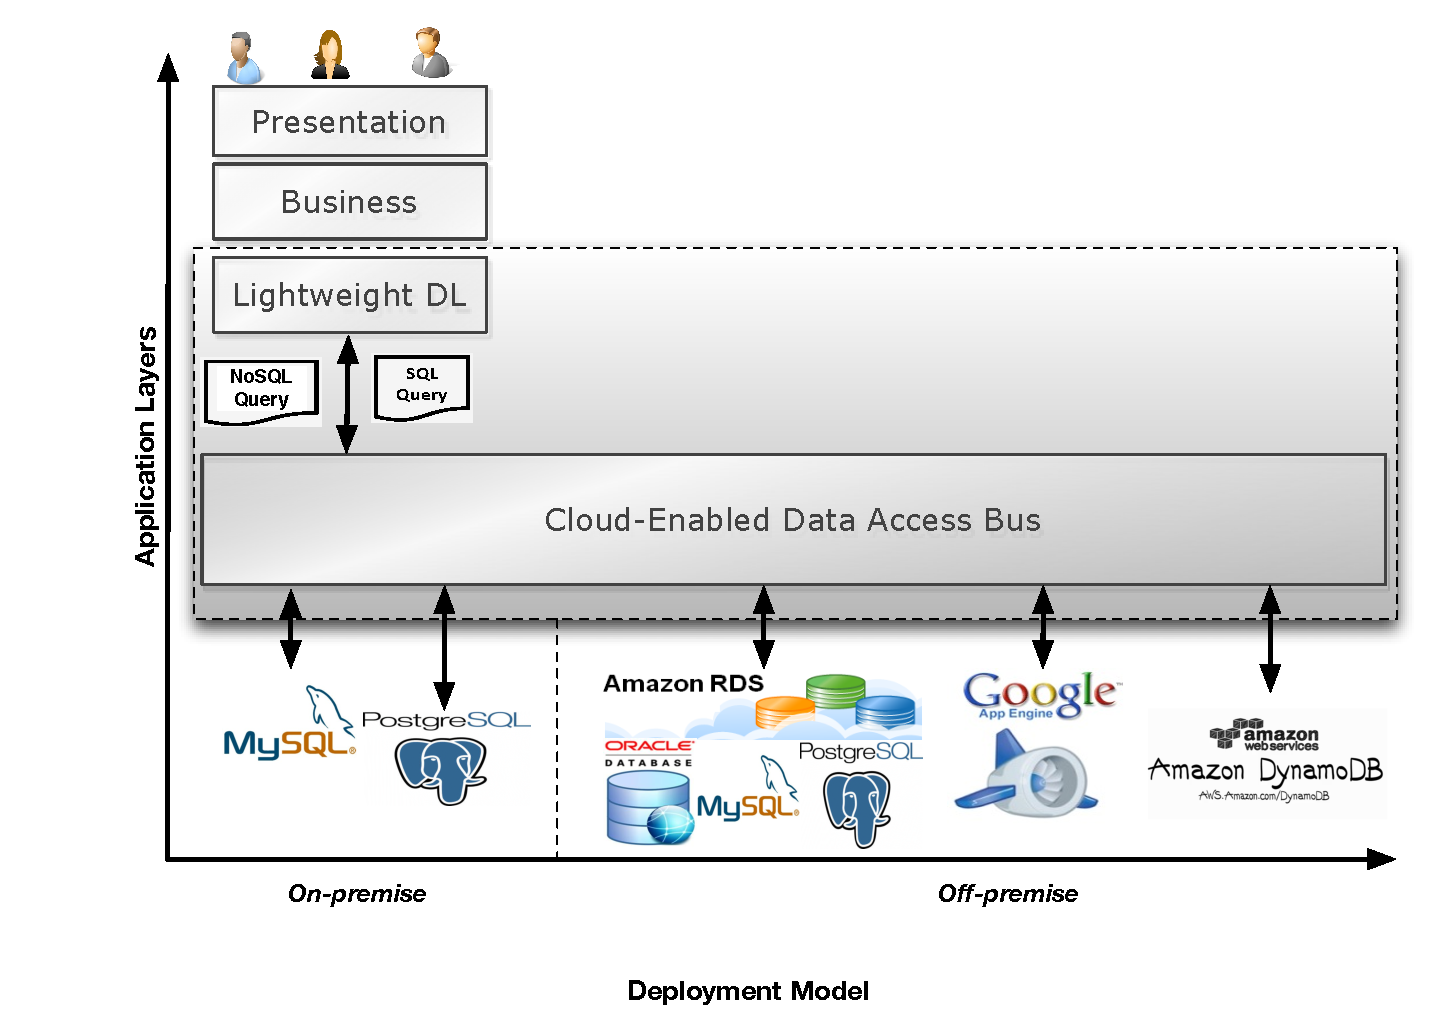
\includegraphics[width=0.925\textwidth, trim=0.0cm 0.0cm 0.0cm 0.0cm, clip]{./gfx/motivationScenario.pdf}
	\caption[Migration Scenario]{Migration Scenario to be filled }
	\label{fig:motivationscenario}
\end{figure}

As shown in Figure \ref{fig:motivationscenario}, the Cloud-Enabled Data Access bus provides access support between the hosted on-premise, and off-premise application's layers. Its main goal is to provide communication isolation between different applications and users, and maintain the transparency that the DL provided before the migration to the upper layers of the application's architecture. Support must be provided for two different databases types: MySQL and NoSQL databases, and between different providers. A tenant who migrates its data, e.g. to the Google SQL Datastore in Google App Engine, as shown in Figure \ref{fig:motivationscenario}, must be able to access his data with minimum adaptations of the components. Furthermore, storing or retrieving data whose storage is divided into multiple datasources requires a dynamic routing between backend data stores. Compatibility between different SQL and NoSQL databases must be also ensured. However, query and data transformation between different data sources types is out of the scope of this diploma thesis.  


\FloatBarrier
\section{Definitions and Conventions}
\label{sec:definitions}

In the following section we list the definitions and the abbreviations used in this diploma thesis for understanding the description of the work.

\subsection*{Definitions}

\subsection*{List of Abbreviations}

The following list contains abbreviations which are used in this document. 

\begin{acronym}[ApacheODEX]
\acro{ACID}{Atomicity, Consistency, Isolation, Durability}
              \acro{API}{Application Programming Interface}
	\acro{ASP}{Application Service Provider}
	\acro{Axis2}{Apache eXtensible Interaction System v. 2}
	\acro{BC}{Binding Component}
	\acro{BLOB}{Binary Large Object}
		\acro{BPEL}{Business Process Execution Language 2.0}
	\acro{C-CAST CMF}{Project Context Casting (C-CAST) Context-Management Framework}
		\acro{CLI}{Command-line Interface}
	\acro{CLOB}{Character Large Object}
	    \acro{CORBA}{Common Object Request Broker Architecture}
	         \acro{DBaaS}{Database-as-a-Service}
	           \acro{DBMS}{Database Management System}
	             \acro{DBS}{Database System}
	                  \acro{DCOM}{Distributed Component Object Model}
	                      \acro{DCE}{Distributed Computing Environment}
	\acro{EAI}{Enterprise Application Integration}
	\acro{EAR}{Enterprise Archive}
	\acro{EJB}{Enteprise JavaBeans}
	             \acro{EIP}{Enterprise Integration Patterns}
	\acro{ESB}{Enterprise Service Bus}
	        \acro{GAE}{Google App Engine}
	            \acro{HTTP}{Hypertext Transfer Protocol}
	\acro{IaaS}{Infrastructure-as-a-Service}
	\acro{IDE}{Integrated Development Environment}
	\acro{JAR}{Java Archive}
	\acro{Java EE 5}{Java Platform, Enterprise Edition v. 5}
	      \acro{J2EE}{Java 2 Platform, Enterprise Edition}
    \acro{JAX-WS}{Java API for XML-Based Web Services}
    \acro{JAXB}{Java Architecture for XML Binding}
	\acro{JBI}{Java Business Integration}
	\acro{JBIMulti2}{JBI Multi-tenancy Multi-container Support}
	\acro{JDBC}{Java Database Connectivity}
	\acro{JDK}{Java Development Kit}
	\acro{JMS}{Java Message Service}
	\acro{JMX}{Java Management Extensions}
	         \acro{JNDI}{Java Naming and Directory Interface} 
	\acro{JOnAS}{Java Open Application Server}
	\acro{JPA}{Java Persistence API}
	             \acro{JSON}{JavaScript Object Notation}
	\acro{JSF}{JavaServer Faces}
	\acro{JVM}{Java Virtual Machine}
	        \acro{LRU}{Least Recently Used} 
	\acro{MBean}{Managed Bean}
		\acro{MDBS}{Multidatabase System}
		       \acro{MEP}{Message Exchange Patterns}
		             \acro{MOM}{Message-Oriented Middleware}
	\acro{NIST}{National Institute of Standards and Technology}
	       \acro{NM}{Normalized Message}
	        \acro{NMF}{Normalized Message Format}
	\acro{NMR}{Normalized Message Router}
	               \acro{NoSQL}{Not only Structured Query Language}
	\acrodep{OSGi}{Open Services Gateway initiative}
	             \acro{ORDBMS}{Object-relational Database Management System}
	\acro{PaaS}{Platform-as-a-Service}
	\acro{POJO}{Plain Old Java Object}
	        \acro{POM}{Project Object Model}
	\acro{QoS}{Quality of Service}
	             \acro{RDBMS}{Relational Database Management System}
	                    \acro{SA}{Service Assembly}
	\acro{SaaS}{Software-as-a-Service}
    \acro{SE}{Service Engine}
            \acro{SMPP}{Short Message Peer-to-Peer}
            \acro{SNMP}{Simple Network Management Protocols}
	\acro{SOA}{Service-Oriented Architecture}
	\acrodep{SOAP}{Simple Object Access Protocol}
	              \acro{SQL}{Structured Query Language}
	              	          \acro{STaaS}{Storage-as-a-Service}
		                 \acro{SU}{Service Unit}
		\acro{TCP}{Transmission Control Protocol}
		       \acro{URI}{Uniform Resource Identifier}
    \acro{UUID}{Universally Unique Identifier}
    \acro{W3C}{World Wide Web Consortium}
            \acro{WAR}{Web Application Archive} 
    \acro{WS*}{Web Services (Specifications)}\acused{WS*}
    \acro{WSDL}{Web Services Description Language}
    \acro{WSS4J}{Apache Web Services Security for Java}
    \acro{XML}{eXtensible Markup Language}
    \acro{XSD}{XML Schema Definition}
    \acro{XSLT}{Extensible Stylesheet Language Transformation}
             

            

\end{acronym}
\section{Outline}
\label{sec:outline}

The remainder of this document is structured as follows:

\begin{itemize}
\item \textbf{Fundamentals, Chapter \ref{chap:fundamentals}:} provides the necessary background on the different concepts, technologies, and prototypes used in this diploma thesis.
\item \textbf{Related Works, Chapter \ref{chap:relatedworks}:} discusses relevant State of the Art and positions our work towards it.  
\item \textbf{Concept and Specification, Chapter \ref{chap:spec}:} functional and non-functional requirements are discussed in this section.
\item \textbf{Design, Chapter \ref{chap:design}:} gives a detailed overview of the differerent component's architecture, and the needed extensions to the already existing ones.
\item \textbf{Implementation, Chapter \ref{chap:implementation}:} the implemented components, as well as the necessary extensions or changes are detailed in this section from the point of view of coding and configuration. 
\item \textbf{Validation and Evaluation, Chapter \ref{chap:validationevaluation}:} in this chapter we test the final prototype based on the scenario described in this document. 
\item \textbf{Outcome and Future Work, Chapter \ref{chap:outcome}:} we provide a conclusion of the developed work and investigate some ideas in which this diploma thesis can be extended.
\end{itemize}
\chapter{Fundamentals}
\label{chap:fundamentals}

In this chapter we give an explanation about the technologies and concepts this diploma thesis relies on. We start describing the fundamental concepts and introduce the components and prototypes that form the basis of our work.

\section{Cloud Computing}
\label{sec:cloudcomputing}

In the last decades our world has become more and more interconnected. This interconnection added to the increase of the available bandwidth and the change in business models have forced IT Systems to fulfill its demands, leading to its reorganization into a public utility which offers public services, like water, electricity, etc. The \ac{NIST} defines Cloud computing as "a model for enabling ubiquitous, convenient, on-demand network access to a shared pool of configurable computing resources (e.g., networks, servers, storage, applications, and services) that can be rapidly provisioned and released with minimal management effort or service provider interaction"  \cite{NIST2011}. The Cloud computing model is composed of five characteristics:
	\begin{enumerate}
		\item On-demand self-service: a Cloud user consumes the Cloud provider's computing capabilities automatically without the need of human interaction. 
		\item Broad network access: computing capabilities are available via the network and can be accessed using standard mechanisms.
		\item Resource pooling: computing capabilities in the Cloud provider side are virtualized to serve multiple consumers simultaneously using a multi-tenant model. The Cloud consumer generally has no sense of the provided resources.
		\item Rapid Elasticity: computing and storage resources can be dynamically (and in some cases automatically) provisioned and released to respond to the actual consumers' demand.
		\item Measured Service: resources' usage is monitored and measured in a transparent way to the Cloud consumer and provider for control and optimization purposes.
	\end{enumerate}

The control that the Cloud consumer has over the computer resources in a Cloud provider infrastructure is defined in three service models: \term{\ac{SaaS}}, \term{Platform-as-a-Service (\ac{PaaS})} and \term{\ac{IaaS}}. \term{\ac{SaaS}} provides to the Cloud consumer access and usage of Cloud provider's applications running on a Cloud infrastructure. The consumer has no control over the underlying infrastructure where the application he uses is deployed. The customer can only control individual application's configurations during his usage of it. \term{\ac{PaaS}} provides the customer with the needed capabilities to deploy applications which's programming language, required libraries, services and tools are supported by the provider. The consumer has no control over the underlying infrastructure where he deploys the application. \term{\ac{IaaS}} is the model which gives most control to the consumer. Thus, the consumer is able to deploy and run arbitrary software and has the control over operating systems, storage and deployed applications, but has no management or control on the underlaying Cloud infrastructure. 

Although the three service models described above provide both data computation and storage capabilities for the consumer, they do not provide to the customer the possibility to directly and uniquely purchase access of storage services. In this diploma thesis we concentrate in two concrete models: \term{\ac{DBaaS}} and \term{\ac{STaaS}}. Cloud storage providers target a selected number of consumers, who process their data on-premise, but do not  want to cover the expenses of a local database system, or a backup system, among others. The Cloud storage model alleviates the need in organizations to invest in database hardware and software, to deal with software upgrades, and to maintain a professional team for its support and maintenance \cite{dbaasIyer}.  \ac{DBaaS} and \ac{STaaS} can be considered quite similar, except for one of their main distinction characteristics: their access interface. The former is the most robust data solution offered as a service, as it offers a full-blown database functionality. It can be accessed via the most common database protocols, such us MySQL, Oracle, etc, or by REST interfaces supporting \ac{SQL}. Examples of this model are Amazon RDS \cite{amazonrds} and Oracle Cloud \cite{oraclecloud}. On the other hand, the latter provides REST, \ac{SOAP} over \ac{HTTP}, or Web-based interfaces in order to perform the operations over the stored data \cite{cloudstorageWU}. Examples of this model are Amazon Dynamo \cite{amazondynamodb} , Google App Engine Datastore \cite{googleappdatastore}, and Dropbox \cite{dropbox}.

\ac{NIST} defines four deployment models in Cloud computing. A private Cloud consists in a Cloud infrastructure which is provisioned exclusively for one organization and used by the members conforming the organization. It is comparable to processing facilities that are enhanced with the Cloud computing characteristics. A community Cloud is a Cloud infrastructure where its use is limited to organizations which share the same requirements. A public Cloud infrastructure can be accessed and used by the public. It is usually offered by Cloud service providers that sell Cloud services made for general public or enterprises. Some of the Cloud consumers may process and store information which requires more control over the infrastructure in which is located, or consume public Cloud computing resources during peak loads in their private Cloud infrastructure. The hybrid Cloud model combines two or more deployment models described above and the combination remains as a unique entity.  

Cloud computing and \ac{SOA} are related styles at an architectural, solution and service level, according to IBM \cite{IBM2011}. Cloud providers expose their Cloud infrastructure as services as part of a \ac{SOA} solutions and the communication between Clouds in the Hybrid Cloud model described above can be compared to a SOA communication solution between enterprises. Cloud services are services that can be accessed by the Cloud consumers through the network. Therefore, we can deduce that the SOA model can be applied in the Cloud computing approach. As the \ac{ESB} is the central piece of \ac{SOA}, the need of the \ac{ESB} in a Cloud computing infrastructure as an integration middleware for the Cloud services is essential. 
\section{Service-Oriented Architecture}
\label{sec:soa}  

Weerawarana et al. define SOA as an specific architectural style that is concerned with loose coupling and dynamic binding between services \cite{Weera2005}.

In the last years communication between external components whose functionalities are exposed as services has been a hard task when there was not previous agreement on message protocols, data types and encoding, and used middleware technology. Due to the economic and technological growth needed, enterprises had to adapt the \ac{SOA} paradigm in their existing IT Infrastructure. \ac{SOA} provides the needed flexibility by building an architectural style with the following benefits: loose coupling, interoperability, efficiency, and standardization. The W3C group defines SOA as a form of distributed system architecture that is typically characterized by the following properties \cite{w3csoa}:
	\begin{itemize}
		\item Logical view: the service's functionality is exposed, but not its internal logic.
		\item Message orientation: the internal structure of an agent is abstracted.
		\item Description orientation: a service is described by machine-processable meta data.
		\item Granularity: services tend to use a small number of operations with relatively large and complex messages.
		\item Network orientation: Services tend to be oriented toward use over a network.
		\item Platform neutral: Messages are sent in a platform-neutral, standardized format delivered through the interfaces.
	\end{itemize}

\ac{SOA} defines three main roles: requester, provider and broker and the four main operations: publish, find, bind, and invoke. The service provider provides access to services, creates a description of a service and publishes it to the service broker. The service requestor discovers a service by searching through the service descriptions located in the service broker. When the service which best fits to his needs is found, the discovering facility provides the concrete service endpoint and the consumer is responsible for binding to it.  With this information, the requestor can then bind to the concrete service and finally execute a business activity \cite{Weera2005}. The service broker provides support for service registration and binding. 

The main component in a \ac{SOA} is the \ac{ESB}. The functionalities provided by a service bus can simplify the process (publication, discovery, binding, and invocation) and make it more transparent to provide an ease-to-use experience for a Web service based implementation of \ac{SOA} \cite{Weera2005}. Chappel defines its function as an intermediate connection provisioning of service providers with service consumers and thereby ensure decoupling of theses \cite{Chapp2004}. 

\subsection{Enterprise Service Bus}

The flow of data and information is a key for driving business decisions in IT organizations \cite{Chapp2004}. Furthermore, the interaction between loosely coupled components within an organization or with third party organizations requires distributed systems mechanisms which provide communication support for different protocols, and reliability. SOA has fulfilled this main requirement by providing an integration environment with minimal (or any) integration efforts. 

The \ac{ESB} is the central component in \ac{SOA}. It provides a loosely coupled, event-driven \ac{SOA} with a highly distributed universe of named routing destinations across a multi-protocol message bus \cite{Chapp2004}. An \ac{ESB} provides an abstract decoupling between connected applications by creating logical endpoints which are exposed as services and conform a multi-protocol environment, where routing and data transformation are transparent to the service connected to it. Furthermore, when using an \ac{ESB}, in the first place, services are configured rather than coded, demanding minimal adaptation, implementation and maintenance efforts. The programmer just has to implement the binding to the logical endpoint exposed as a service. In the second place, \ac{ESB} routing is based on a reliable messaging router. Applications don't need to include message system-failure forwarding mechanisms, to know which data formats are needed in the consumed services, or to care about future changes in applications or services the applications interact with. An \ac{ESB} hides the complexity of orchestration between services in business processes. 

Chappel defines the combination of loosely coupled interfaces and asynchronous interactions as a key concept of the bus terminology  \cite{Chapp2004}. A user of the bus can access every service registered in the bus. For this purpose, it implements the \ac{SOA} operations in order to make them transparent to the user who can therefore focus on: plugging to the bus and posting and receiving data from the bus. Furthermore, the \ac{ESB} can form the core of a pervasive grid \cite{Chapp2004}. Services supported by an organization can be organized between the \ac{ESB}s conforming the grid, as well as its access between the organizational departments, and services provided to third party organizations. 

%\begin{figure}[htb]
%	\centering
%		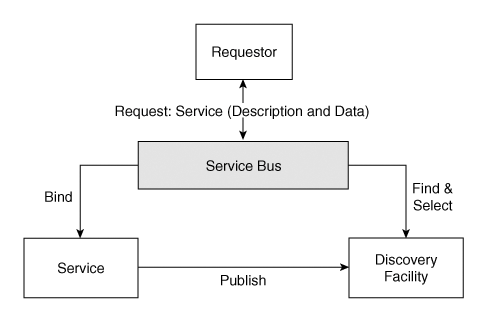
\includegraphics[clip, scale=0.7]{./gfx/servicebus.png}
%	\caption[The Role of the service bus in SOA]{The Role of the service bus in \ac{SOA} \cite{Weera2005} }
%	\label{fig:servicebus}
%\end{figure}

%(see Figure \ref{fig:servicebus})

When receiving a service description (\ac{WSDL}) and data from the service requester, the \ac{ESB} is responsible for selecting the service which best fits to the description requirements, for binding the service requester with the backend service through a route created between the logical endpoints and for making the necessary data transformations to enable the communication between the parts.

As the \ac{ESB} is the central component in \ac{SOA}, and established as integration middleware for services, in this diploma thesis we focus on the required modifications and extensions in the open-source \ac{ESB} Apache ServiceMix 4.3 to provide transparent communication support between the applications and its data located in on-premise databases, or migrated to off-premise data stores. 

\FloatBarrier
\section{Multi-tenancy}
\label{sec:specificationmultitenancy}

In this section we detail the multi-tenant requirements the system must fulfill in order to ensure tenant-isolation at two levels: communication and storage. The final prototype must ensure a multi-tenant aware transparent access to data hosted in the Cloud. Although we provide storage support in our system for hosting migrated tenant's data (see Section \ref{sec:systemoverview}), it does not implement a multi-tenant storage model, because this is not a goal in our design. Therefore, we rely on the multi-tenant storage models different Cloud providers implement.

\subsection{Communication Requirements}

The final prototype must not only support a multi-tenant, but also a multi-protocol communication between endpoints. ServiceMix-mt is shipped with the following multi-tenant aware \ac{BC}s: \ac{HTTP}, \ac{JMS}, and E-mail \cite{gomez2012}. However, the existing communication protocols for data transfer purposes leads us to discard the \ac{JMS} and E-mail. \ac{RDBMS}, e.g. MySQL and PostgreSQL, implement their own protocol in their client/server model, at the \ac{TCP} level of the network stack. At the client side the protocol is supported by the native drivers provided to the developers, e.g. MySQL Connector/J, and at the server side by the different components which build the database server \cite{mysqlmanual}. This fact forces us to provide a vendor-oriented communication protocol environment, by providing support for the different protocols in independent components, rather than in a single standardized component.

Communication in, and from the \ac{ESB} must be multi-tenant aware. We divide the required isolation between tenants into the following sub-requirements: 

	\begin{itemize}
		\item \textbf{Tenant-aware messaging}: messages received in the \ac{ESB} and routed between the tenant-aware endpoints should be enriched with tenant and user information. 
		\item \textbf{Tenant-aware endpoints}: in ServiceMix-mt tenants pack a common endpoint configuration packed in a \ac{SU}, which is then deployed as a \ac{SA} in ServiceMix-mt's \ac{JBI} container \cite{gomez2012}. The multi-tenant aware \ac{BC} dynamically modify the endpoint's URL by injecting tenant context in it. In a database system in our scenario we do not have only tenants as the main actors, but also the different users which can access a tenant's database. Therefore, the tenant-aware endpoints should be dynamically created by injecting tenant and user information in the endpoint's URL. Furthermore, we must ensure tenant and user authentication in the system. 
		\item \textbf{Tenant-aware routing and context}: the deployment of tenant-aware endpoints should be followed by the creation of a tenant-aware context. Resources involved in a routing operation from one consumer endpoint to one provider endpoint can be shared between different tenants, but they must manage the routing operations in different tenant-aware contexts. The routing operations between two endpoints must identity the tenant and user who initiated the routing. 
		\item \textbf{Tenant configuration isolation}: configuration data persisted in our system should be isolated between tenants. A tenant's endpoint configuration data contains sensible information which identifies and allows access to the tenant's backend data stores. 
		\item \textbf{Tenant-aware correlation}: in a request-response operations, the response obtained from the backend data store must be correlated with the tenant's request to the system, and ensure that one tenant does not receive responses from another tenant's request.
	\end{itemize}

\subsection{Storage Requirements}

Due to the fact that our system does not primarily requires multi-tenant aware storage support, but we rely on multi-tenant aware storage systems in the Cloud, we summarize the main requirements for isolating data between tenants in database systems. 

Curino et al. identify as a primary requirement for a Cloud provider offering a \ac{DBaaS} model security and privacy \cite{relationalcloud2010}. A system running multiple database servers and each server multiple database instances must contain the necessary meta-data to provide tenant-aware routing in the system, and ensure that one tenant can only access the information in his database instance. Furthermore, privacy of stored data between tenants can be ensure by encrypting all tuples \cite{relationalcloud2}. Curino et al. introduce \term{CryptDB}, a subsystem of a relational Cloud which provide data encryption and unencryption functionalities for persisting data, and for accessing data via \ac{SQL} queries which are not aware of the encrypted storage mechanism in the system. However, it is known that the key challenge in managing encrypted data in the Cloud is doing it efficiently.

\FloatBarrier
\section{Java Business Integration}
\label{sec:jbi}

The interaction between enterprises' applications has suffered in the past from lack of standardized technologies, leading each of the enterprises to develop their own or acquiring vendor-specific integration technology. \ac{JBI} is defined by the Java Community as an integration technology which maximizes the decoupling between components and defines an interoperation semantic founded on standards-based messaging. This allows different vendor-specific components to interoperate in a multivendor "echosystem" \cite{JBI2005}. 

The key which leads to the integration of different components relies on a unique message format in the \ac{JBI} environment which different plugged-in components use to communicate within the environment. External components are not directly connected, but through a mediator. The communication mediator between components in a \ac{JBI} environment is the \ac{NMR}. Its main functionality is the routing of the internal standardized \ac{NM} between the components. However, it can perform additional processing during the message exchange. The \ac{NMR} fields are defined as an \ac{XML} document format payload, metadata conforming the header and a non \ac{XML} document format attachment referenced by the payload.

The \ac{JBI} specification defines two different types of components which are categorized in two types and provide different services:
	\begin{itemize}
		\item A \ac{SE} provides transformation and composition services to other components.
		\item A \ac{BC} provides the connectivity between the external services and the \ac{JBI} environment. They support many different protocols and isolate the \ac{JBI} environment by marshaling and demarshaling the incoming or outgoing message into the internal standardized \ac{NM} format.
	\end{itemize} 
	
Both components listed above can function as service consumers or service providers following a \ac{WSDL}-based, service-oriented model. The consumer endpoint provides a service accessible through an endpoint which can be consumed by other components, while the provider endpoint consumes a functionality exposed as a service and accessible through an external endpoint. The routing of \ac{NM} starts when a message exchange between components is created (bidirectional communication pipe, a \term{DeliveryChannel}, between the communicating endpoints) and continues with the target of the specified service endpoint for processing (see Figure \ref{fig:jbi}). The \ac{NMR} supports four asynchronous message exchange patterns differing in the reliability and direction of the communication.

\begin{figure}[htb]
	\centering
		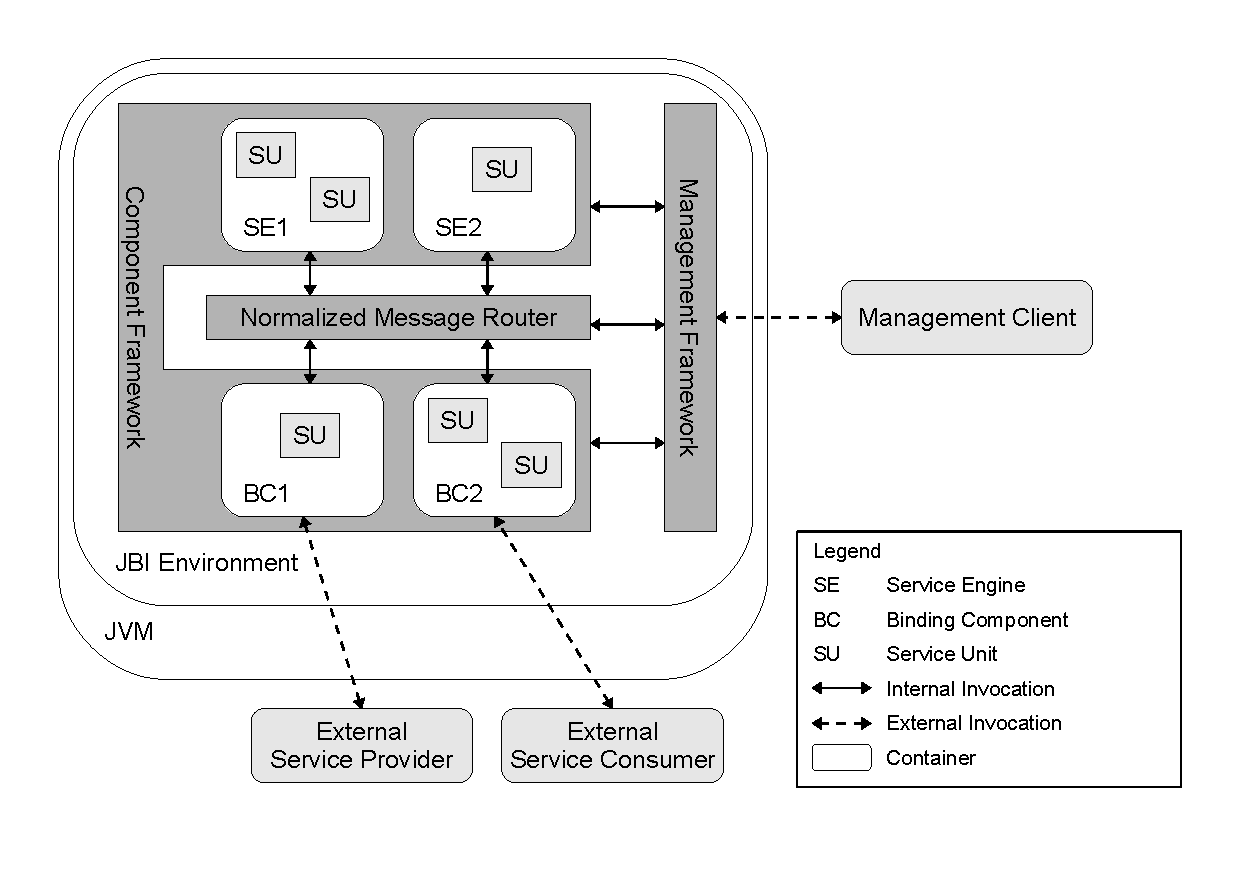
\includegraphics[width=0.85\textwidth, trim=0.95cm 0.95cm 0.95cm 0.95cm, clip]{./gfx/JBIArchitecture.pdf}
	\caption[JBI Architecture]{Overview of JBI Architecture. Figure 4 in JBI specification document \cite{JBI2005}.}
	\label{fig:jbi}
\end{figure}

In Figure \ref{fig:jbi} we can observe that one or more \ac{SU} are contained in a \ac{BC}. The \ac{SU}s are component-specific artifacts to be installed to a \ac{SE} or a \ac{BC} \cite{JBI2005}. The service units are packed in a \ac{SA}, usually as ZIP files, where it is specified each of the components where each of the \ac{SU}s should be deployed. The \ac{JBI} environment provides a Java Management Extension \ac{JMX} Framework for installation, life cycle management, addition, and monitoring and control of the components conforming to the environment defined by the JBI specification.

\FloatBarrier
\section{OSGi Framework}
\label{sec:osgi}

The \ac{OSGi} framework provides loose coupling between modules in a Java environment. It provides a strong support for module versioning and third party modules referencing. The \ac{OSGi} defines a framework for deployment support in a \ac{JVM} of downloaded or extended resources known as \term{bundles}. This framework requires OSGi-friendly devices a minimum system's resources usage by providing dynamic code-loading and \term{bundle} lifecycle management. An \ac{OSGi} \term{bundle} is the packaging of a group of Java classes and required and provided capabilities' meta-data as a JAR file for providing functionality to end users, which can be exposed as bundle services or just run internal processes. A valid \ac{OSGi} bundle can be installed in any valid \ac{OSGi} container due to the standardized packaging and bundle management. 

\ac{OSGi} \term{bundles} can be downloaded, extended and installed remotely or locally in the platform when needed without the need of system reboot. Installation and update of bundles during their lifecycle are also managed by the framework, which uses a service registration for selection, update notifications, or registry of new service objects offered by a deployed bundle. This feature is the main key for connecting bundles whose's services require during runtime capabilities provided by another bundles. The framework defines a bundle's requirement capability as a dependency.      

The \ac{OSGi} framework defines 5 different layers and a bundle's lifecycle \cite{OSGi2011}. An optional Security Layer provides the infrastructure for deploying and managing applications which must be controlled during runtime. The Module Layer lists the rules for package sharing between the deployed bundles. The lifecycle of a bundle can be modified during runtime through an API provided in the lifecycle layer. The main operations implemented are install, update, start, stop or uninstall. 

Apache ServiceMix 4.3.0 is built on and \ac{OSGi}-based runtime kernel, which provides a lightweight container that enables the deployment of various bundles \cite{openesbaction}. Its architecture and functionalities are described in the following section. 

\section{Apache ServiceMix}
\label{sec:servicemix}  

In this diploma thesis we extend a multi-tenant aware version of Apache ServiceMix 4.3.0, referred to it in this document as ServiceMix. Essl evaluates different available \ac{ESB} solutions in the market, and as output of his work provides a selection decision for extending ServiceMix in order to support multi-tenancy \cite{Essl2011}. As mentioned in Section \ref{sec:multitenancy}, a multi-tenant \ac{ESB} solution in a \ac{PaaS} environment must support tenant-aware communication, and tenant-aware administration and management. The support is provided by Muhler and Gomez in their corresponding works in \cite{Muhler2012}, \cite{gomez2012}, leading to a multi-tenant ServiceMix prototype supporting different communication protocols. We will refer to it as ServiceMix-mt.

As a main difference with previous versions' architectures, ServiceMix is an integration container based on the \ac{OSGi} Framework implementation Apache Karaf  \cite{Karaf2011}. It provides a light environment in which components and applications can be deployed in a loose coupled way. Apache Karaf provides an extensible management command line console where management of the components lifecycle, such us \ac{OSGi} bundles, \ac{JBI} components or \ac{SA}s, can be done in a user friendly way (see Figure \ref{fig:servicemix}). Furthermore, a hot deployment directory is shipped with the \ac{ESB} package where users can deploy \ac{OSGi} bundles, \ac{JBI} components wrapped in \ac{SA}'s, etc. just by copying the file into it. The undeployment is done automatically when the user deletes the file from the \term{deploy} directory. 

The main advantage in the ServiceMix 4.3.0 it is its full compliance with the \ac{JBI} specification. Its \ac{JBI} container has as its main component the \ac{NMR} (See Figure \ref{fig:servicemix}). In the \ac{JBI} container users are provided with \ac{JBI} deployment support and management. The communication between the \ac{JBI} and \ac{OSGi} container, e.g. from one \ac{OSGi} service to a \ac{JBI} Binding Component can be achieved through the \ac{NMR} using its API wrapped as an already deployed \ac{OSGi} bundle. This fact eases the integration process of components between different ServiceMix's versions, and take advantage of it in this diploma thesis. Furthermore, \ac{JBI} components or endpoint configurations packed as \ac{SE} or \ac{SA} and deployed in ServiceMix are internally packed into \ac{OSGi} bundles. 

ServiceMix is shipped with different \ac{JBI} components already deployed as \ac{OSGi} bundles in its \ac{OSGi} container. In this thesis we will concentrate on the following ones: HTTP and Apache Camel. Apache Camel is a powerful open source integration framework based on \ac{EAI} \cite{Camel2011}. Furthermore, it provides a widespread list of components which support different communication protocols.  The user can configure logical endpoints between \ac{BC}s and different routing paths between them by deploying their configuration wrapped in a \ac{SA} in the \term{deploy} directory. Different Maven plugins can make the configuration of a \ac{JBI} or \ac{SE} as simple as possible by providing different built archetypes which generates the \ac{SU} files and directories where the developer can configure the component \cite{MAVEN}. Apache Camel provides a set of maven archetypes which already contain the structure for developing custom camel components.

\begin{figure}[htb]
	\centering
		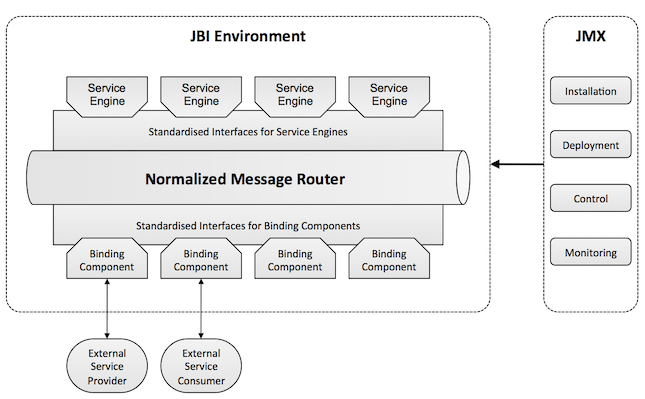
\includegraphics[clip, scale=0.4]{./gfx/servicemix.png}
	\caption[Architecture of Apache ServiceMix]{Architecture of Apache ServiceMix \cite{ASM} }
	\label{fig:servicemix}
\end{figure}

The \ac{NMR} routes the messages between the endpoints created by the \ac{JBI} components (see Figure \ref{fig:servicemix}). This endpoints are divided in two types: consumers and providers. A consumer endpoint is exposed as a service while a provider endpoint consumes an external service. When a message arrives to a consumer endpoint of a \ac{JBI} Binding Component, it is transformed into a \ac{NMF}. The \ac{NMF} is the protocol neutral format which is routed in a \ac{JBI} environment and described in Section \ref{sec:jbi}. 

The ServiceMix-mt prototype we extend in this diploma thesis already provides multi-tenant support for different communication protocols: HTTP, JMS, and E-mail. However, the data retrieval and storage in an application's architecture relies on one specific layer: Data Access Layer, and its main used communication protocols for data transfer are in most of the cases vendor specific. Communication with \ac{SQL} databases, such as MySQL, Oracle, and PostgreSQL are managed by its vendor-specific native driver, which implements the communication protocol with the database server in the \ac{DBMS}. Such protocols are not supported in the multi-tenant prototype ServiceMix-mt, and must be taken into account in the extension of the prototype in this diploma thesis. On the other hand, communication with \ac{NoSQL} databases can be also considered vendor-specific, because most of the Cloud storage providers facilitate its own API to the users to manipulate data in their data containers, but almost all of them provide either REST or \ac{SOAP} over \ac{HTTP} interfaces. This fact permits us to reuse and extend the multi-tenant HTTP \ac{BC} in ServiceMix-mt. The components we create or extend in this diploma thesis are identified by CDASMix (Cloud Data Access Support in ServiceMix-mt).

\FloatBarrier
\section{Binding Components}
\label{sec:bindingcomponents}  

In this section we describe the \ac{JBI} \ac{BC}s shipped in the ServiceMix-mt prototype this diploma thesis focuses on, and the transport protocols they support. 

\subsection{Multi-tenant HTTP Binding Component}

ServiceMix provides \ac{HTTP} communication support in its \ac{HTTP} \ac{JBI} \ac{BC}. Its \ac{HTTP} consumer and provider endpoints are built on the \ac{HTTP} Jetty 6 server and Jakarta Commons \ac{HTTP} Client respectively, providing support for both REST and SOAP over HTTP 1.1 and 1.2 requests.

The original \ac{HTTP} \ac{BC} is extended in the ServiceMix-mt prototype to provide multi-tenant support in \cite{Muhler2012} and \cite{gomez2012}. Muhler provides an internal dynamic creation of tenant-aware endpoints in the \ac{BC}, by injecting tenant context in the \ac{JBI} endpoint's URLs \cite{Muhler2012}. Gomez provides a \ac{NMF} with tenant context information in its properties for routing in the \ac{NMR} \cite{gomez2012}. However, in this diploma thesis we must not only provide tenant isolation at the tenant level, but also isolation at the user level. We discuss this requirement in detail in Chapters \ref{chap:spec} and \ref{chap:design}.

\begin{figure}[htb]
	\centering
		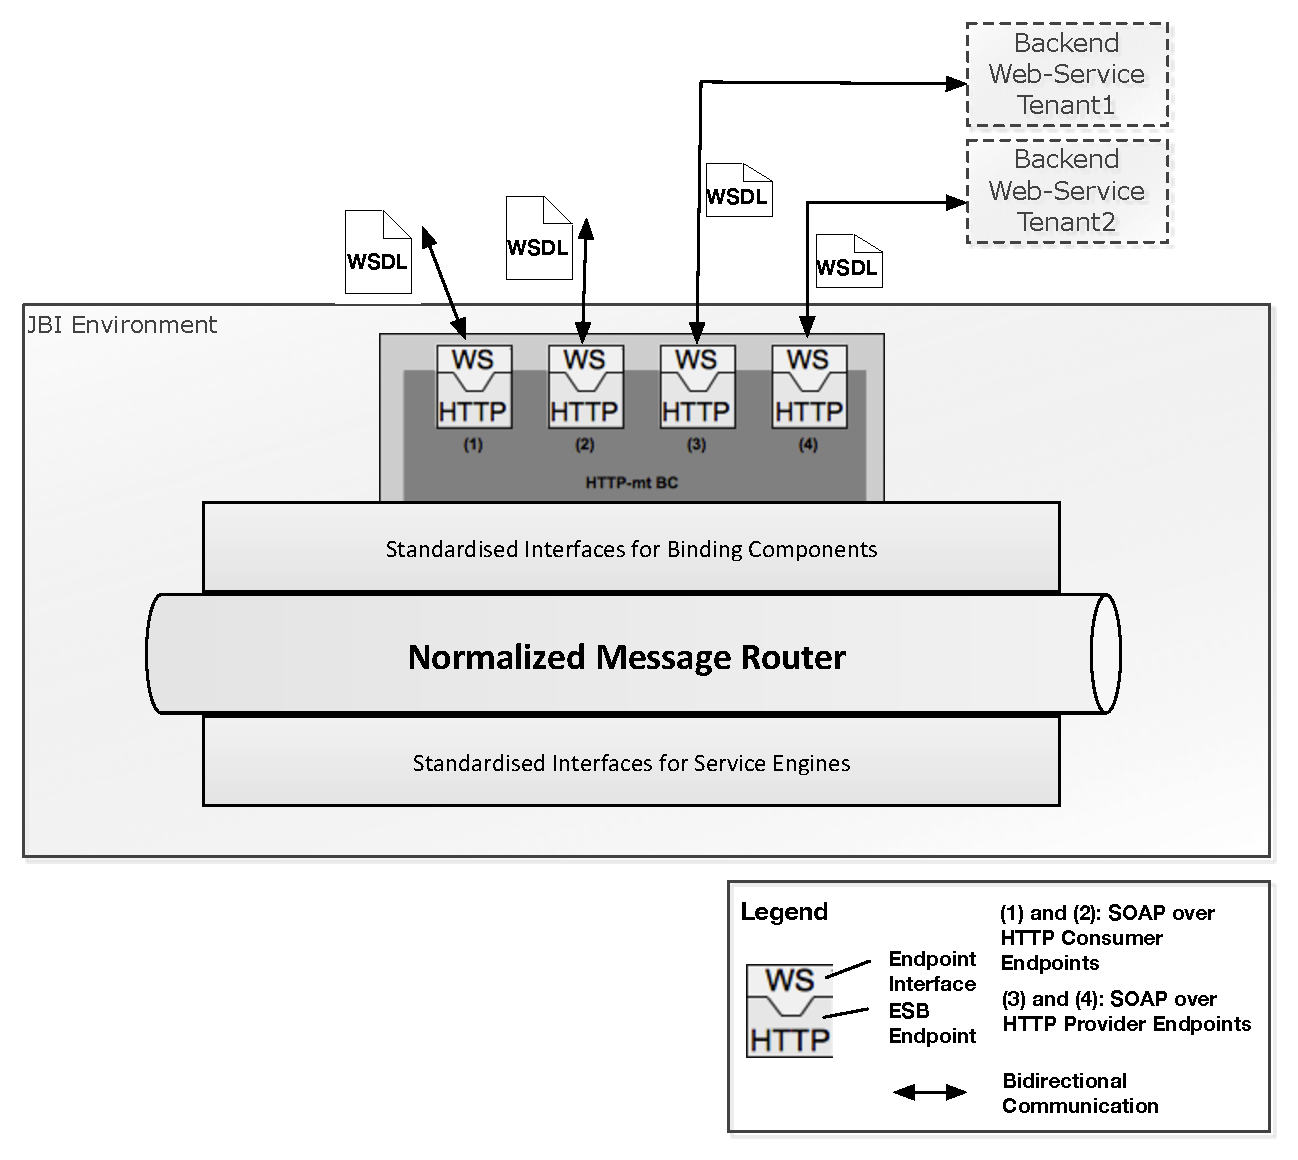
\includegraphics[clip, scale=0.3]{./gfx/httpmtbc.pdf}
	\caption[Multi-tenant HTTP Binding Component]{Multi-tenant HTTP Binding Component \cite{gomez2012}. }
	\label{fig:httpmt}
\end{figure}

As seen in Figure \ref{fig:httpmt}, the multi-tenant \ac{HTTP} \ac{BC} is mainly used in ServiceMix-mt to support the \ac{SOAP} over \ac{HTTP} communication protocol by exposing a Web service in the tenant-aware consumer endpoint and consuming an external Web service in the provider endpoint. \ac{SOAP} defines an \ac{XML} message format  which is sent over the network and a set of rules for processing the \ac{SOAP} message in the different \ac{SOAP} nodes which build the message path between two endpoints \cite{Weera2005}. A \ac{SOAP} message is a composition of three main elements: a SOAP envelope, header, and body. A SOAP envelope may contain zero or more headers and one body. The header may contain processing or authentication data for the ultimate receiver or for the intermediate nodes through the message is routed. The message payload or business data is included in the SOAP body. SOAP is used as a message framework for accessing Web services in loosely coupled infrastructures \cite{Weera2005}. The Web service consumer specifies the functionality to invoke in the SOAP body. If the Web service functionality has a request-response \ac{MEP}, a SOAP message is used to send the response data when the corresponding operation has been executed successfully or the error data in case an error occurred during execution.

Most of the Cloud storage providers provide an \ac{HTTP} interface to the tenants for data management, retrieval, and storage. In this diploma thesis we extend this \ac{JBI} \ac{BC} in order to provide the tenant a transparent access to his \ac{NoSQL} Cloud data stores.

\FloatBarrier

\section{Service Engine}
\label{sec:serviceengine}  

A \ac{SE} can provide different kinds of services, e.g. business logic, routing, and message transformation. In this diploma thesis we will mainly concentrate on one: Apache Camel \cite{Camel2011}, which is wrapped in a ServiceMix-camel \ac{JBI} \ac{SE} in ServiceMix, and in a ServiceMix-camel-mt \ac{JBI} \ac{SE} in ServiceMix-mt  for multi-tenancy awareness..

\subsection{Apache Camel}

Apache Camel is an open-source integration framework based on known \ac{EIP} which supports the creation of routes and mediation rules in either a Java based Domain Specific Language (or Fluent API), via Spring based XML Configuration files or via the Scala DSL \cite{Camel2011}. In ServiceMix, Apache Camel is shipped in a \ac{JBI} \ac{SE}. The routing or mediation rules between two or more endpoints can be specified in an Spring Configuration file or in a \ac{POJO} file whose's class extends the Apache Camel \term{RouteBuilder} class. Route configurations deployed in ServiceMix must follow the \ac{JBI} compliance: files describing the route configuration must be packed in \ac{SU}, and the latter in a \ac{SA}. Apache Camel provides Maven archetypes which generate the needed route configuration files (in \ac{XML} or \ac{POJO} formats) where the developer can program the route between the different supported endpoints \cite{MAVEN}. The configuration in a \ac{XML} file reduces the configuration complexity to a minimum effort of the developer. However, a configuration in a \ac{POJO} class increases the developing complexity but allows the developer to provide logic, filtering, dynamic routing, etc. In the \term{RouteBuilder} class a developer can access, for example, the header of a \ac{NM} and select the target endpoint dynamically depending on the implemented logic. Furthermore, the routing patterns supported by Apache Camel are the point-to-point routing and the publish/subscribe model. 

The endpoints representation in Apache Camel is based on \ac{URI}. This allows this \ac{SE}s to integrate with any messaging transport protocol supported in the \ac{ESB}, e.g. \ac{HTTP}, \ac{JMS} via ActiveMQ, E-Mail, CXF, etc. The ServiceMix-camel \ac{JBI} \ac{SE} provides integration support between camel and \ac{JBI} endpoints. Muhler extends this component and allows dynamic internal creation of tenant-aware endpoints in the ServiceMix-camel-mt \ac{JBI} \ac{SE} \cite{Muhler2012}. The main goal of this extension is to provide an integrated environment between \ac{JBI} and camel supported endpoints. However, multi-tenancy is supported at the tenant level only in the \ac{JBI} endpoints. In this diploma thesis we aim to enable multi-tenancy not only at the tenant level, but also at the user level, as discussed in Chapters \ref{chap:spec} and \ref{chap:design}.

For enabling data access support with \ac{SQL} \ac{DBMS} in ServiceMix-mt we extend a well-known camel component: Camel-jdbc. The Camel-jdbc component enables \ac{JDBC} access to \ac{SQL} databases, using the standard \ac{JDBC} API, where queries and operations are sent in the message body \cite{cameljdbc}. This component requires the developer to statically denote the data source configuration (user, password, database name, etc.) in both the endpoint \ac{URI} and route configuration file. As discussed in Chapters \ref{chap:spec} and \ref{chap:design}, this requirement is opposite to our approach, due to the dynamism we need in creating connections to the different \ac{DBaaS} providers. We extend and produce a custom camel component: Camel-jdbccdasmix (\term{cdasmix} stands for Cloud Data Access Support in ServiceMix-mt).

\FloatBarrier

\section{SQL Support Architectural Overview}
\label{sec:designsql}

In this section we provide an overview of a preliminary, and final architectural approaches designed in this diploma thesis, in order to support a transparent data access to backend \ac{SQL} databases. We first expose the integration approaches we should consider, and the main problems found when implementing the first approach which led us to design a second architectural approach. 


\subsection{Integration}

%integration of osgi and jbi in terms of messaging
%integration of osgi and jbi in terms of containers and libraries
%explain why we have two approaches
%jbi components offered in servicmix are deployed as osgi bundles
% jbi components offered in servicemix-mt are deployed as jbi component, and internally wrapped into an osgi bundle
% may have to put a figure of the contents in both of the packages so that we can see. It is all about the meta inf library where the bundle manifest info is exposed
As described in Chapter \ref{chap:spec}, we build the new components in ServiceMix-mt following the \ac{OSGi} compliance. However, these must interact with components which follow the \ac{JBI} specification. The integration between components built for different containers in ServiceMix-mt must be done at two levels: messaging, and resources sharing. The ServiceMix-mt \ac{NMR} \ac{API} \ac{OSGi} bundle exposes a set of operations for sending messages through the \ac{NMR} to a specified target endpoint. Hereby we can perform message exchanges between endpoints configured on \ac{OSGi} bundles and endpoints configured on \ac{JBI} components, and provide communication support between components hosted in the two containers. 

\begin{figure}[htb]
	\centering
		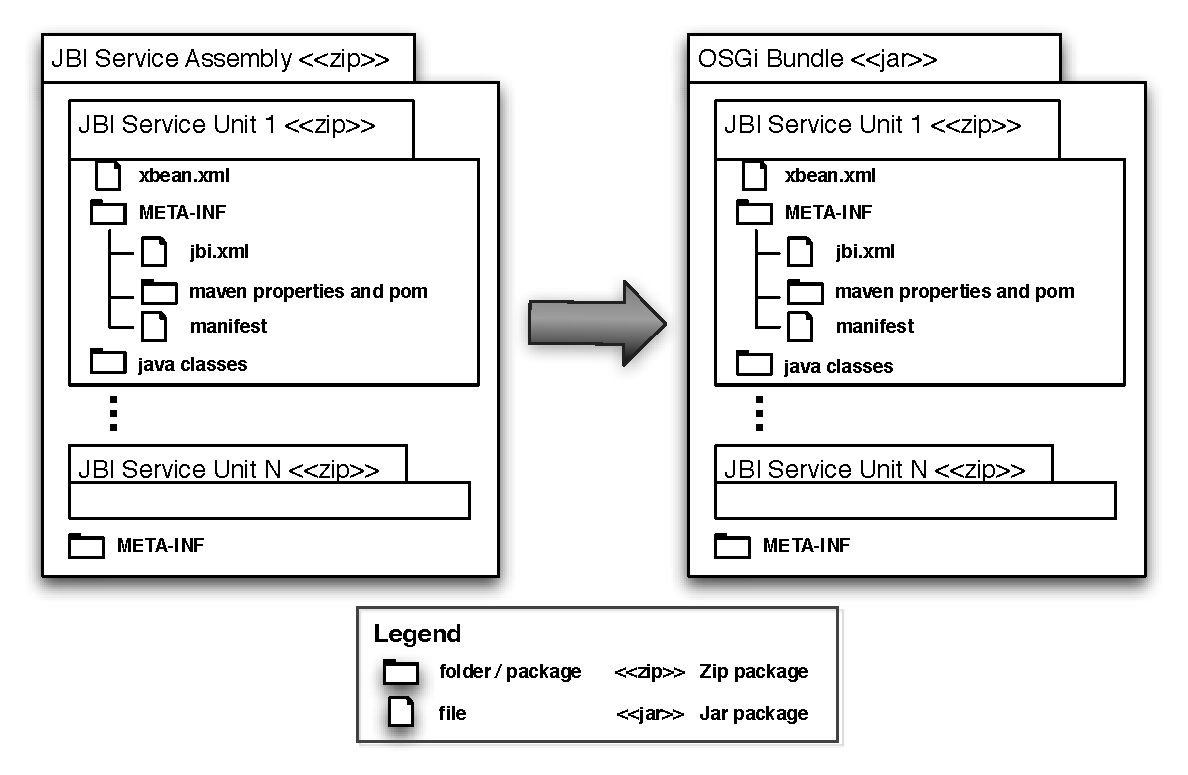
\includegraphics[clip, scale=0.5]{./gfx/osgibundlepackage.pdf}
	\caption[JBI to OSGi repackaging]{ServiceMix 4.x repackaging mechanism for deploying \ac{JBI} components in \ac{OSGi} container.}
	\label{fig:jbitoosgipackage}
\end{figure}

The resources sharing integration level refers to the deployment of \ac{JBI} components in the \ac{OSGi} container, and the utilization of packages exposed by \ac{OSGi} bundles in the \ac{OSGi} container in a loosely coupled manner. The former is part of the integration between containers provided in ServiceMix 4.x versions and described in Figure \ref{fig:jbitoosgipackage}. The deployment mechanism of a \ac{JBI} \ac{SA} into an \ac{OSGi} container is simple: repackaging of the \ac{SA} as a JAR. However, this cannot be consider a full integration in the \ac{OSGi} container. \ac{OSGi} bundles contain in their \term{META-INF} folder one fundamental file for the \ac{OSGi} kernel: the \term{manifest} file. This contains a description of the bundle, the packages it imports, and exports. Imported packages can be either statically stored in the bundle or imported from third party bundles, and exported packages are the ones which exposed to third party bundles. These can be imported with an internal class loading mechanisms developed in the \ac{OSGi} container. The repackaging of the \ac{SA} into a JAR, as it is shown in Figure \ref{fig:jbitoosgipackage}, contains the \term{META-INF} folder, and the \term{manifest} file. However, the latter only contains information about the author, date of creation, but it does not contain information related to the exported packages, and the needed packages to be imported. This \term{manifest} file describes the \ac{SA}, and not the \ac{SU}s. Java classes and package importing description are contained in the \ac{SU} package, and not in the \ac{SA} package. Therefore, the \ac{OSGi} container cannot register in its registry the packages it exports as a service, and cannot load the imported packages to the bundle context. This fact forces us to statically include in the \ac{SA}, and the \ac{SU} the packages which are referenced in each \ac{SU}, and leads to scalability constraints with the tenant-aware deployment process of the system.

ServiceMix 4.x versions are shipped with different \ac{JBI} \ac{BC}s packed as an \ac{OSGi} bundle. However, they are deployed as \ac{OSGi} bundles, and not as \ac{SA}s, in order to enable loose coupling and package sharing between components in the \ac{OSGi} container. ServiceMix-mt allows the deployment of the \ac{JBI} \ac{BC}s, but deployment of \ac{JBI} \ac{BC}s as OSGi bundles is not supported in the JBIMulti2 application. This lack of support forces us to design a second architectural approach, as described in the following sections.

\FloatBarrier

\subsection{Approach 1}

\ac{SQL} database systems provide access to their databases through an endpoint, which is represented as an URL. The native driver used in the data access layer of an application connects to the endpoint, authenticates, sends the query, and reads the response. Therefore, we must support in our system the same operational steps. As discussed in this diploma thesis, the communication protocol varies between different vendors. In this diploma thesis we provide support for incoming MySQL messages. Tenants must access our system through a single physical endpoint. This endpoint is provided by a MySQL proxy which is enriched with authentication, cashing, marshaling, and demarshaling operations. As shown in Figure \ref{fig:designsqlapp1}, the MySQL Proxy Bundle implements the MySQL server operations which are related with the client/server communication protocol. In Figure \ref{fig:designsqlapp1} we specify a server running on port 3306. However, this value can be configured before the deployment of the \ac{OSGi} component. This component is built as an \ac{OSGi} bundle and its packages are exported as services in the \ac{OSGi} container. It interacts with three different components in the system: the \ac{NMR} \ac{API}, the Cache, and the Service Registry. 

Cashing mechanisms are implemented in both the Registry-Cache, and the MySQL Proxy Bundle. The former provides an \ac{API} for creating cache instances, and for persisting and retrieving data. We create a separate cache instance for the \ac{SQL} support due to the need of a custom key creation mechanism which may not coexist in a shared cache between different bundles, as well as the needed isolation of sensible tenant configuration information from third party bundles. The system provides a set of operations which ease the creation of multi-tenant aware keys for persisting frontend authentication data, and queries results form the backend database systems. 

The \ac{NMR} \ac{API} is shipped in ServiceMix as an \ac{OSGi} bundle which exports its \ac{API} as an \ac{OSGi} service. The set of operations included in its \ac{API} allows \ac{OSGi} bundles to create, send, and receive message exchanges to \ac{JBI} endpoints (see Figure \ref{fig:designsqlapp1}).  Before creating the message exchange, the MySQL Proxy Bundle must build dynamically the target endpoint's URL by injecting the tenant context information, and service and endpoint name.

\begin{figure}[htb]
	\centering
		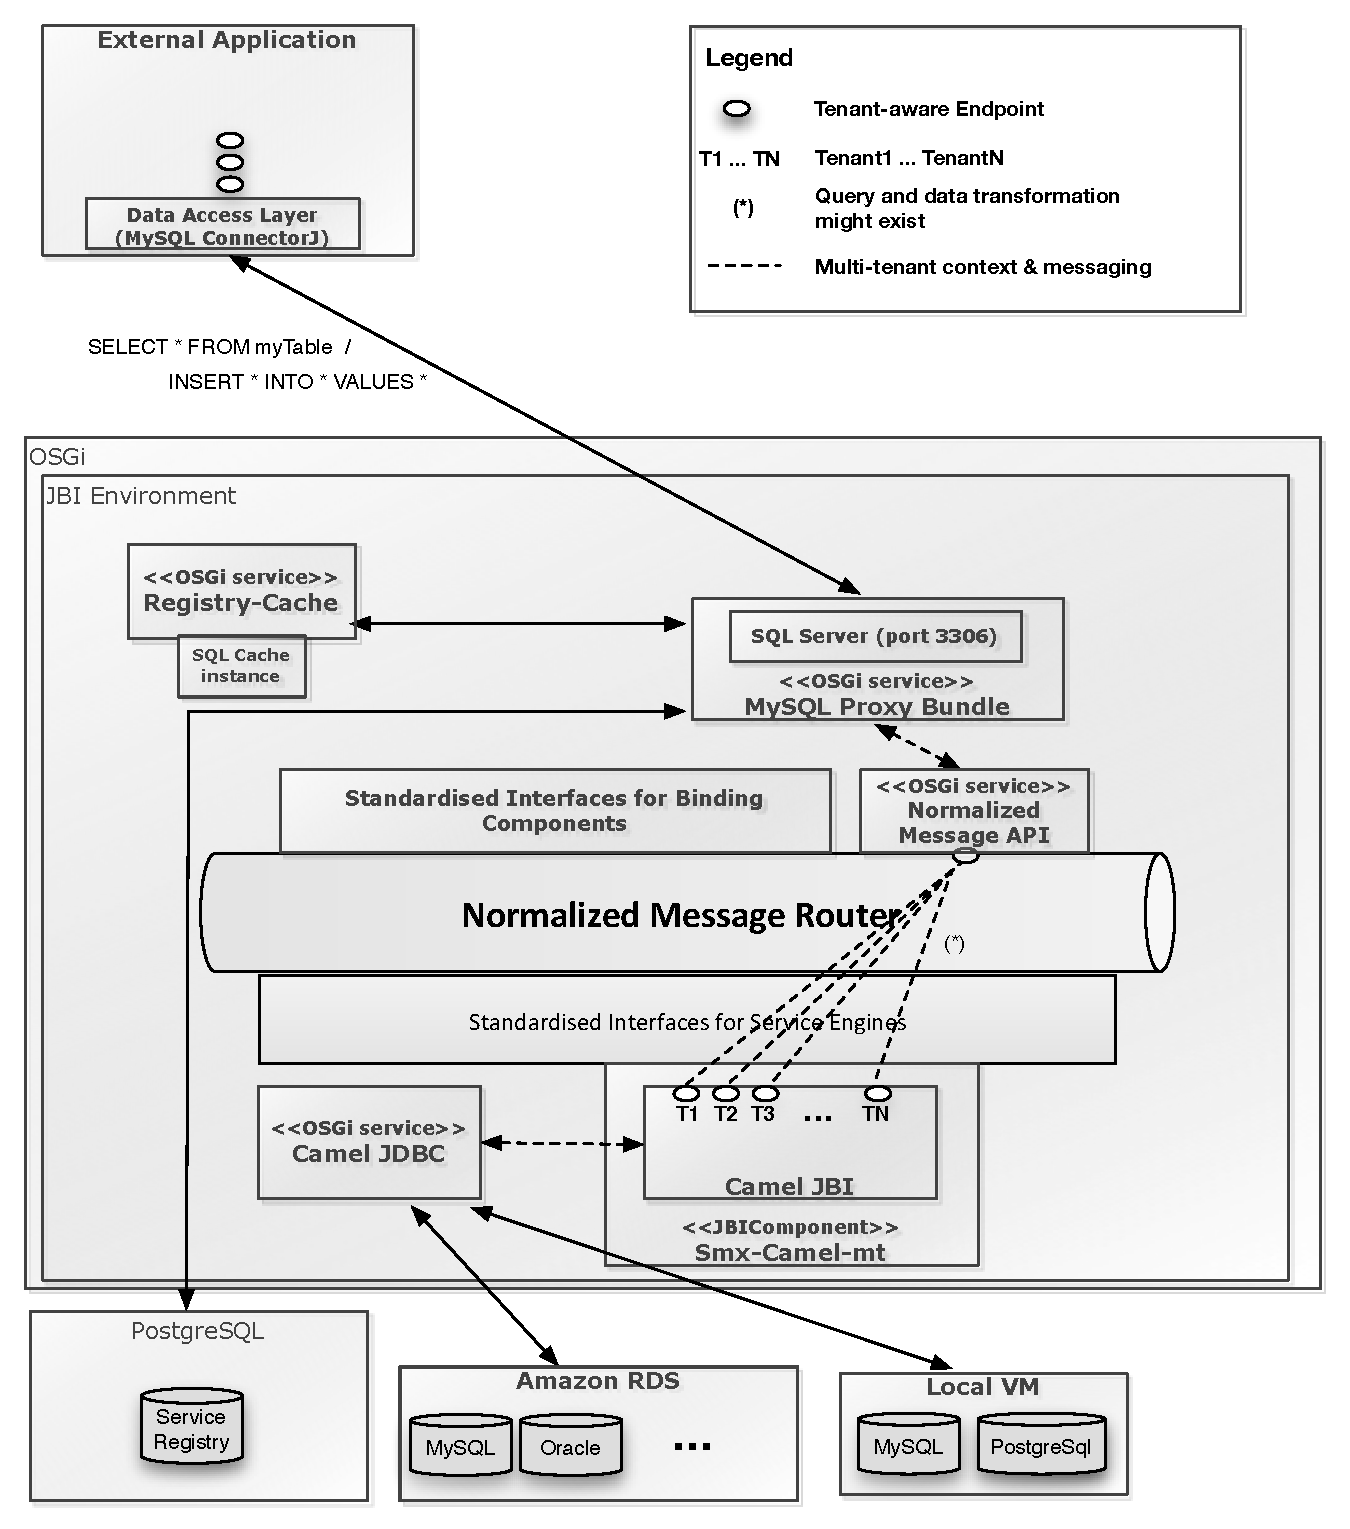
\includegraphics[clip, scale=0.6]{./gfx/sqlApproach/sqlApproachv2_doc.pdf}
	\caption[SQL Support Approach 1]{Architectural overview of the design approach one to support the MySQL communication protocol and routing to backend \ac{SQL} databases.}
	\label{fig:designsqlapp1}
\end{figure}

Apache Camel provides a set of components which integrate most of the communication technologies available in the market. Moreover, it provides an archetype for creating custom components we use in this diploma thesis. ServiceMix provides a Camel \ac{JBI} \ac{BC} which integrates the \ac{JBI} container with the camel router. Muhler extends this component in ServiceMix-mt and enriches it with multi-tenancy awareness. However, the supported multi-tenancy is at the level of tenants, and not at the level of tenant's users. We extend this component and provide user and tenant isolation between endpoints, by injecting the tenant and user UUID in the endpoint's URI (see Listing \ref{lst:endpointuri}). 

%%%%%%%%%%%%%%%%%%%%%%%%%%%%%
\lstinputlisting[float=htb,label={lst:endpointuri},caption={[Tenant-aware Endpoint Configuration]Extended Tenant-aware endpoint URI in extended Backus-Naur Form (EBNF) \cite{Muhler2012}.},style=ebnf]{./gfx/endpointconfiguration.txt}
%%%%%%%%%%%%%%%%%%%%%%%%%%%%%

With multi-tenancy at the tenant and user level, each user can deploy one \ac{JBI} tenant-aware endpoint in the ServiceMix-Camel-mt \ac{SE}. The routes deployed from each tenant-aware endpoint are performed under a different context, and an instance of the targeted component in the route is created. Therefore, with this approach we provide multi-tenancy at the messaging, endpoint, and routing and component context levels. 

Due to the lack of \ac{JDBC} support in ServiceMix for creating provider endpoints, we develop a custom camel component, and enrich it with \ac{JDBC} support for three database systems: MySQL, Oracle, and PostgreSQL. This component is extensible to more database systems when including its native driver, and is build as an \ac{OSGi} bundle and its packages are exported as an \ac{OSGi} service. Messages received from the \ac{NMR} are demarshaled to the backend database system communication protocol, and the response marshaled, correlated, and sent back to the MySQL Proxy Bundle. The demarshalers in this bundle provide the necessary support for transforming the \ac{NMF} response to a MySQL message.

As described in the previous section, ServiceMix-mt provides \ac{JBI} and \ac{OSGi} support and integration, but with some constraints. \ac{JBI} components cannot import packages from \ac{OSGi} bundles exporting its packages. The Servicemix-Camel-mt \ac{SE} provides integration with the camel router for a set of camel components. The camel manual specifies the need for adding statically the custom component packages in the \ac{JBI} \ac{SU} which contains the route definition. Therefore, this leads us to scalability problems in each of the \ac{SA} deployed by the tenants. The \ac{SA} size increases with the new supported database systems, and forces to redeploy all the \ac{SU}s containing the custom camel component when it is modified. This leads to management, storage capacity, and network capacity inconveniences. Hence, we provide a second, and final approach which is very similar to this one, but utilizing the ServiceMix-camel component deployed as \ac{OSGi} bundle. 

\FloatBarrier

\subsection{Approach 2}

In this second architectural design approach we address the scalability problems caused by the \ac{JBI} package dependencies in the \ac{SU}s described in the previous section. This approach is similar to the first one presented, and its main difference relies on the routing from the tenant-aware \ac{JBI} endpoints to the custom camel component \term{cdasmixjdbc} (see Figures \ref{fig:designsqlapp2} and \ref{fig:designsqlapp1}). The functionalities and operations in the MySQL proxy bundle do not differ with the previous approach.
 
\begin{figure}[htb]
	\centering
		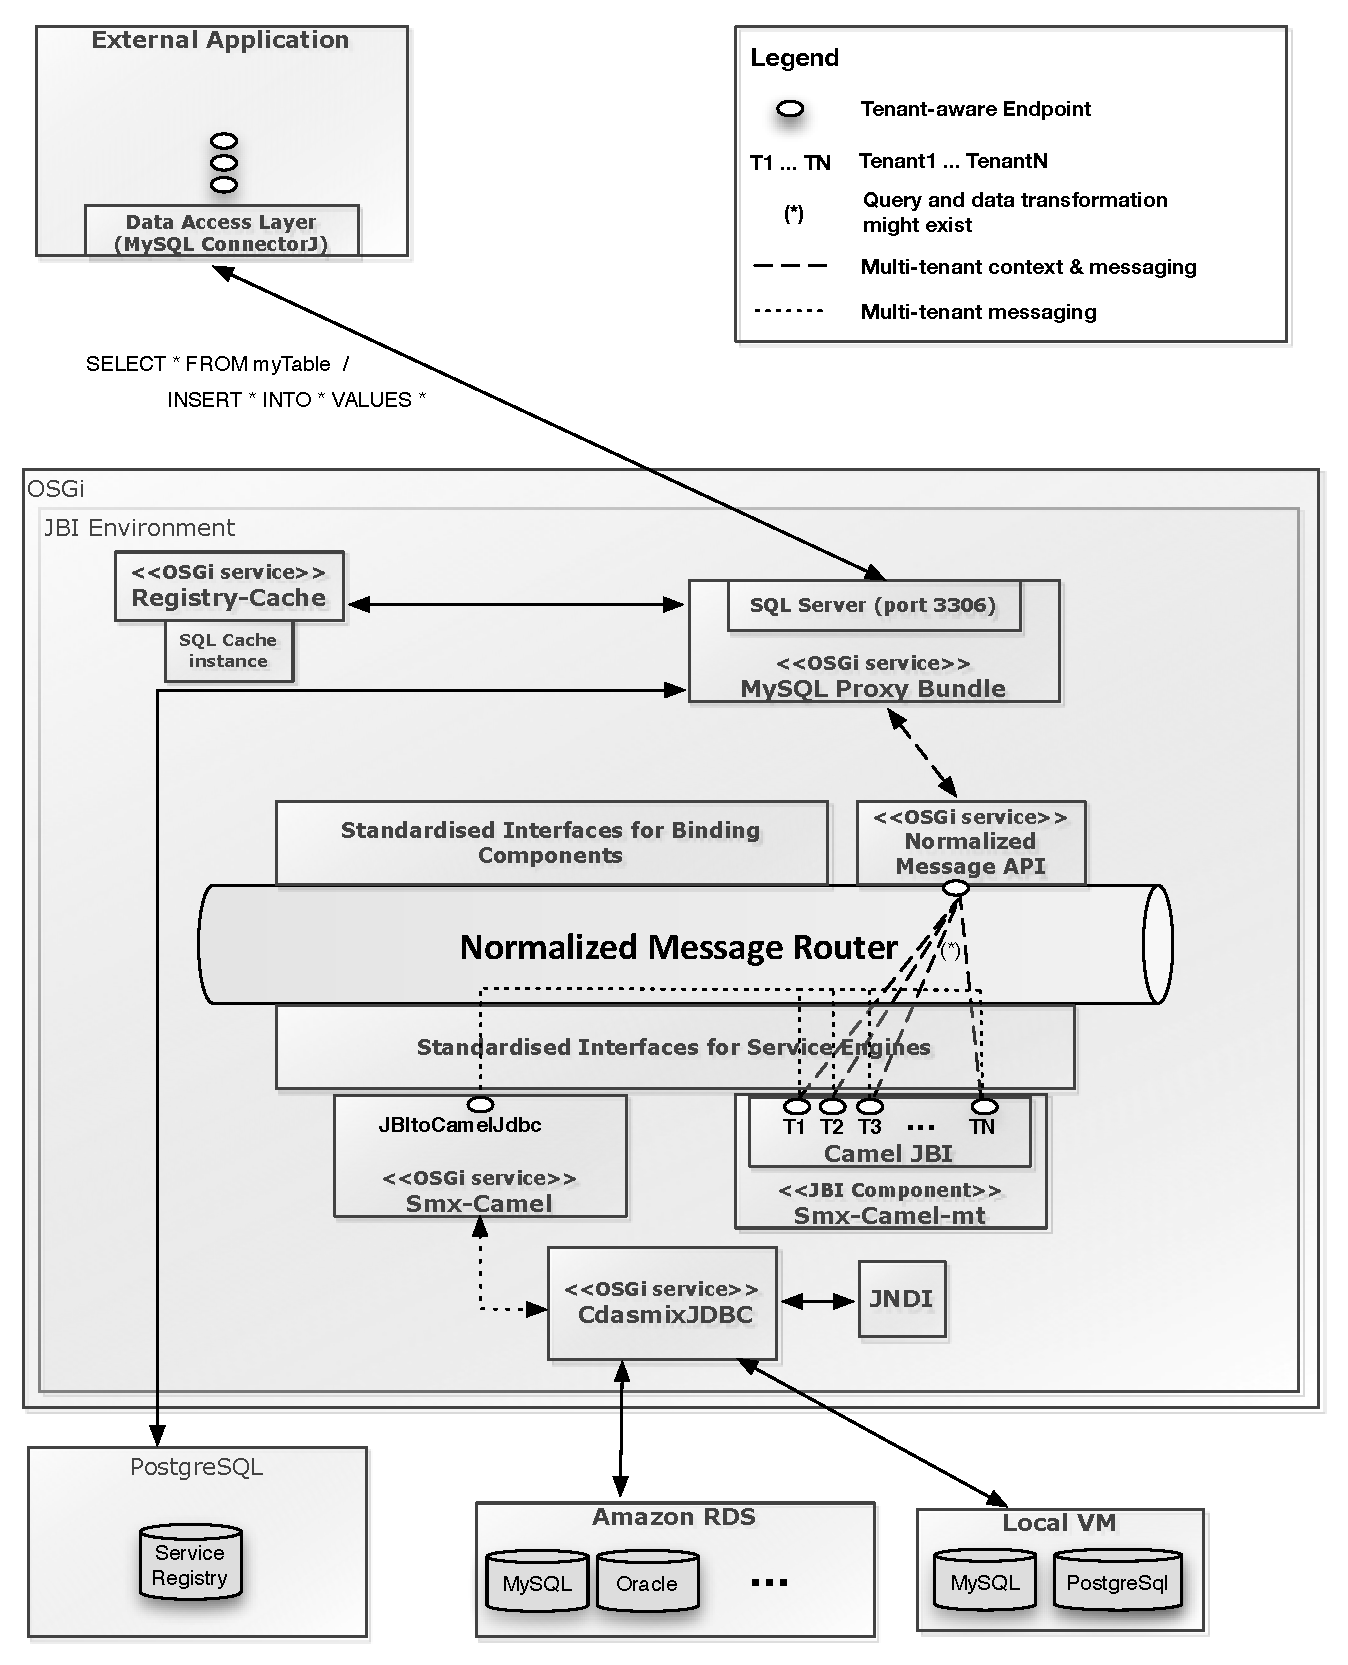
\includegraphics[clip, scale=0.6]{./gfx/sqlApproach/sqlApproachv3_doc.pdf}
	\caption[SQL Support Approach 2]{Architectural overview of the design approach two to support the MySQL communication protocol and routing to backend \ac{SQL} databases.}
	\label{fig:designsqlapp2}
\end{figure}

The message is routed from the MySQL proxy bundle to the tenant-aware \ac{JBI} endpoint deployed in ServiceMix-camel-mt. The multi-tenant message processor instance in ServiceMix-camel-mt routes the message to the \term{JBItoCamelJdbc} endpoint. 

As discussed before, the \ac{JBI} \ac{BC}s deployed in ServiceMix are \ac{OSGi} friendly. This means that the \ac{OSGi} contains a valid manifest file where the description of the bundle, import packages, and export packages are specified. \ac{SU}s deployed on this component are able to reference other \ac{OSGi} packages exposed as a service in the \ac{OSGi} service registry. We provide a single endpoint deployed in the ServiceMix-Camel component where the requests are sent to: the \term{JBItoCamelJdbc} endpoint. When the \term{JBItoCamelJdbc} endpoint is deployed on the ServiceMix-Camel \ac{OSGi} bundle, this searchs in the \ac{OSGi} container for the \term{CdasmixJDBC} component, and creates an instance of the component. Messages routed to the \term{JBItoCamelJdbc} endpoint are then forwarded to the \term{CdasmixJDBC} component, which selects the appropriate \ac{JDBC} native driver, creates a connection, demarshals the request, and forwards the request to the backend Cloud data store server. The connection is established after creating an instance of a \term{DataSource}, which is saved in the \ac{JNDI} registry for future connections, in order to avoid the creation of more than one \term{DataSource} instance per user per backend Cloud data store.

Responses retrieved from the backend Cloud data store are correlated with the initial request and routed back to the MySQL proxy bundle, which demarshals the retrieved data and sends it as a binary \ac{TCP} stream.

In this approach a new instance of the \term{cdasmixjdbc} is not created per tenant endpoint, but is shared between the tenants. Therefore, we cannot ensure an independent component context at the provider endpoint. However, messages contain the tenant information, and the \term{cdasmixjdbc} component interacts with the backend database system establishing separate \ac{JDBC} connections per request. Full multi-tenancy, at the levels of component creation, and endpoint level is not ensured, but it is ensured at the messaging, and context levels. Although full multi-tenancy is not supported, we avoid the deployment of \ac{SU}s which contain the \term{CdasmixJDBC} component in it, and whose size increase may lead to scalability problems in the system. Furthermore, we prevent the deployment of the same component n times, for the n multi-tenant aware endpoints, and prevent future management problems when modifying or upgrading the \term{CdasmixJDBC} component. 

\FloatBarrier



\section{NoSQL Databases}
\label{sec:fundamentalsnosqldb}  

\ac{RDBMS}s ensure data persistency over time and provide a wide set of features. However, the functionalities supported require a complexity, which is sometimes not needed for some applications, and harms important requirements in Web applications or in \ac{SOA} based applications, e.g. throughput. \ac{NoSQL} data stores aim to improve the efficiency of large amount of data storage while reducing its management cost \cite{nosqlcomputerworld}. NoSQL databases are designed to support horizontal scalability without relying on the highly available hardware \cite{strauchnosql}. In a Cloud storage environment where the user sees the available computing and storage resources as unlimited, a \ac{NoSQL} support in a Cloud storage environment might be adequate.

\ac{NoSQL} \ac{DBS} operate as a schema-less storage system, allowing the user to access, modify or freely insert his data without having to make first changes in the data structure \cite{nosql2012}. Cloud providers provide the users with an \ac{API} for accessing, modifying, and inserting data into his isolated container. For example, a user's Amazon Dynamo DB table and item can be accessed by its RESTful \ac{API}, or by installing at the user's side application the Amazon Web Services SDK \cite{amazondynamodb}. Furthermore, it provides the users through its Web-based management console the available management operations. 

Due to the growth of the \ac{NoSQL} support along different Cloud vendors, in this diploma thesis we provide a multi-tenant and transparent communication support for \ac{NoSQL} backend data stores in different Cloud providers. In the following sections we introduce the categorization of the different \ac{NoSQL} databases we aim to support in this diploma thesis, mentioning and giving examples of Cloud data stores available nowadays in the market.

\subsection{Key-value Databases}

In a key-value datastore elements are uniquely identified by an id, which the data store does not take into account its type, and are simply stored as a \ac{BLOB} . A user can get the value for the key, put a value for the key, or delete a key from the data store \cite{nosql2012}. Its storage model can be compared to a map/dictionary \cite{strauchnosql}. Products offering this data storage model in a Cloud infrastructure are Amazon DynamoDB \cite{amazondynamodb}, Google Cloud Storage \cite{googlecloudstorage}, Amazon SimpleDB  \cite{amazonsimpledb} , Amazon S3 \cite{amazons3}, etc. In this diploma thesis we mainly focus on the following key-value data stores: DynamoDB, and Google Cloud Storage.

Amazon DynamoDB's data model includes the following concepts: tables, items, and attributes \cite{amazondynamodb}. The attributes are a key-value, where the value is binary data. Attributes are stored in items, and these are stored in tables. Items stored in a table can be retrieved by referencing its unique id. The number of attributes is not limited by Amazon, but each item must have a maximum size of 64 KB. Accessing stored data in this data store can be mainly done in two ways: using the functionalities provided by the AWS SDK, or using the Cloud storage RESTful \ac{API}. 

Google Cloud Storage's data model includes the following concepts: buckets and objects \cite{googlecloudstorage}. Buckets contain on or more objects. The objects are identified within a bucket with its unique id. Users can perform I/O operations on both buckets and objects. For this purpose, Google Cloud storage provides RESTful \ac{API}.

In this diploma thesis we use an \ac{ESB} for accessing transparently tenant's databases migrated to the Cloud. Servicemix-mt provides multi-tenant \ac{HTTP} support \cite{gomez2012}. Therefore, we reuse and extend the multi-tenant \ac{HTTP} \ac{BC} in order to provide dynamic routing between the different data stores.

\subsection{Document Databases}

Document databases can be considered as a next step in improving the key-value storage model. In this storage model, documents are stored in the value part of the key-value store, making the value content examinable \cite{nosql2012}. Documents with different schemas are supported in the same collection, and can be referenced by the collection's key or by the document's attributes. One of the main difference in the attributes specification regarding \ac{RDBMS} is that in document stores document's attributes cannot be null. When there is an attribute without value, the attribute does not exist in the document's schema. Products implementing this data storage model are Apache CouchDB, MongoDB, etc. \cite{couchdb} \cite{mongodb}.

Mongo DB defines two storage structures: collections and documents \cite{mongodb}. A specific database contains one or more collections identified by its unique id. A specific collection stores one or more documents. Collections and documents stored in a database can be accessed, inserted and modified using the RESTful \ac{API} supported by the database system.

Apache CouchDB defines two storage structures: databases and documents. Data stored in CouchDB are \ac{JSON} documents. The main difference between this two described databases is that MongoDB implements a two step access to the documents: database, collection, and document. Apache CouchDB provides a RESTful \ac{API} for I/O operations.

This databases are not offered by Cloud providers like Amazon or Google, but as a software which can be deployed in user instances, e.g. Amazon EC2 AMI \cite{amazonec2}. 

\subsection{Column-family Stores}

One of the most known Column-family data stores is Cassandra. Column-family data stores store data in column families (groups of related columns which are often accessed together) as rows that have many columns associated with a row key \cite{nosql2012}. This approach allows to store and process data by column instead of by row, providing a higher performance when accessing large amount of data, e.g. allowing the application to access common accessed information in less time.

Cassandra has as its smallest unit of storage the column, which consists of a timestamp and a name-value pair where the name acts as a key \cite{nosql2012}. As in the relational model, a set of columns form up a row, which is identified by a key. A column family is a collection of similar rows. The main difference with the relational model is that each of the rows must not have the same columns, allowing the designer and the application consuming large amounts of data to customize the columns in each row, and the rows in each column family.

Cassandra is not shipped with a RESTful API for I/O operations. However, there are several open-source services layers for Cassandra, e.g. Virgil \cite{virgil}.

\FloatBarrier

\section{JBIMulti2}
\label{sec:jbimulti2}  

A multi-tenant management system must fulfill several requirements, such as data and performance isolation between tenants and users, authentication, specification of different user roles, resources usage monitoring, etc. In a \ac{JBI} environment, endpoint and routing configurations files are packed in \ac{SU}s, and the latter in \ac{SA}s for deployment. However, there is a lack of user-specific data during deployment. Muhler solves this problem in JBIMulti2 by injecting tenant context in the \ac{SA} packages, making them tenant-aware \cite{Muhler2012}. 

\begin{figure}[htb]
	\centering
		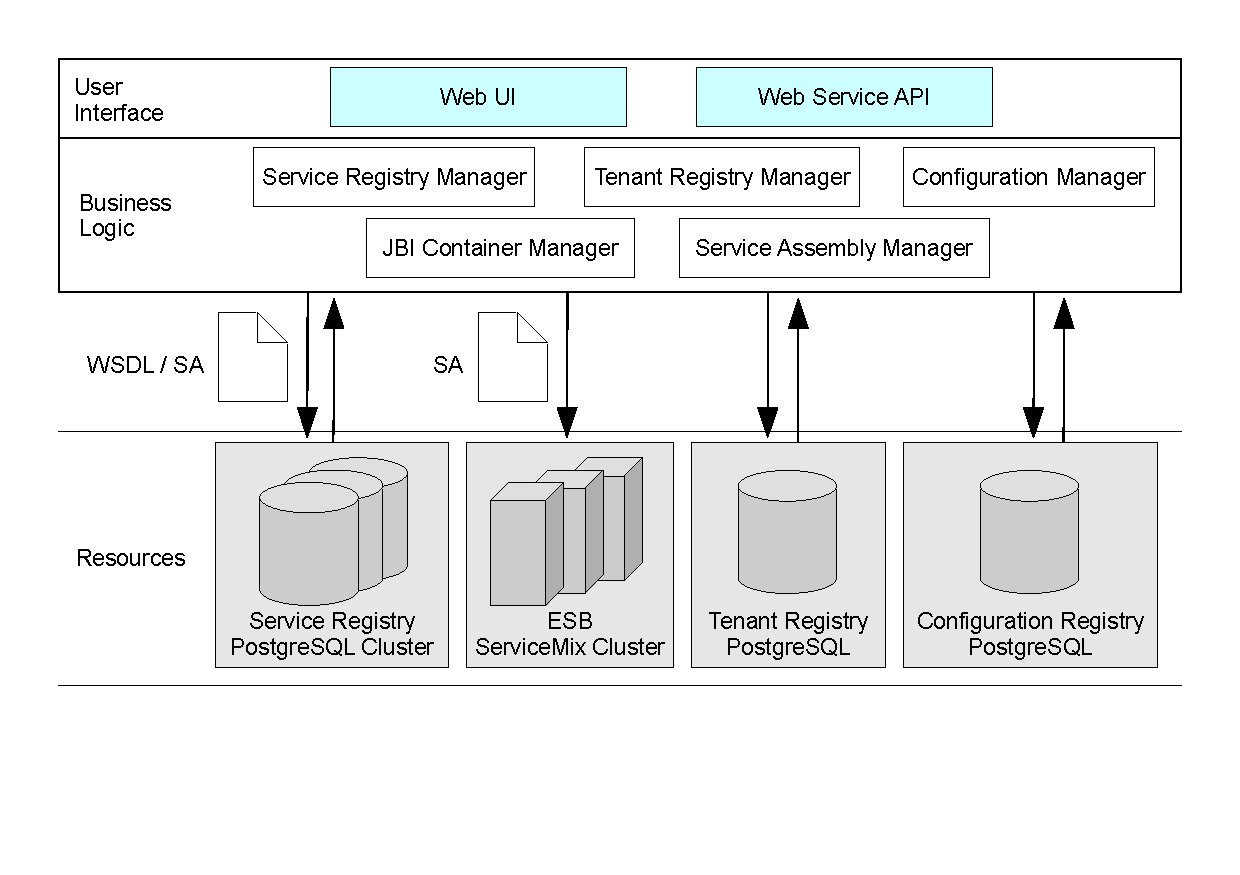
\includegraphics[clip, scale=0.5]{./gfx/systemoverview_jbimulti2.pdf}
	\caption[JBIMulti2 System Overview]{JBIMulti2 System Overview \cite{Muhler2012}} 
	\label{fig:jbimulti2}
\end{figure}

The architecture of the JBIMulti2 system is represented in Figure \ref{fig:jbimulti2}. We can distinguish two main parts in the system: business logic and resources. JBIMulti2 uses three registries for storing configuration and management data. When a tenant (or a tenant user) is registered, an unique identification number is given to them and stored in the Tenant Registry. Both Tenant Registry and Service Registry are designed for storing data of more than one deployed application. The former for storing tenant information and the latter for providing a dynamic service discovery functionality between the different applications accessed through the \ac{ESB}. The Configuration Registry is the key of the tenant isolation requirement of the system. Each of the stored tables are indexed by the tenant id  and user id value. In this thesis we need tenant information during runtime. We reuse and extend the databases schemas produced by Muhler, specifically the Service Registry.

The system provides a user interface for accessing the application's business logic. Through the business logic, the management of tenants can be done by the system administrator or the management of tenant's users can be done by the tenants. Furthermore, when deploying the different tenant's endpoint configurations packed in \ac{SA}s, the system first makes modifications in the zip file for adding tenant context information and then communicates with the Apache ServiceMix instance by using a \ac{JMS} Topic to which all the ServiceMix instances are subscribed to. The \ac{JMS} management service in ServiceMix deploys the received \ac{SA} injected in the received \ac{JMS} message using the administration functionalities provided in ServiceMix. The communication between the business layer and the ServiceMix instance is unidirectional. When successful deployment, the endpoint is reachable by the tenant. When an error occur during deployment, an unprocessed management message is posted in a dead letter queue.

JBIMulti2 requires the previous installation of components, e.g. JOnAS server, PostgreSQL, etc. The initialization of the application is described in both Chapter \ref{chap:validationevaluation} and in the JBIMulti2 setup document \cite{JBIMulti2Man}.
\section{Cloud Data Migration Application}
\label{sec:clouddatamigrationtool}  

The Cloud Data Migration Application provides support to the user before and during the data migration process to the Cloud. It contains a registry of different Cloud data hosting solutions and its properties, which are used during the decision process. The decision process consists in selecting the Cloud provider which best fits the user's operational and economical interests, and in detecting incompatibilities with the selected target data store. The different steps of the migration process are shown in Figure \ref{fig:cloudmigrateapp}. 

\begin{figure}[htb]
	\centering
		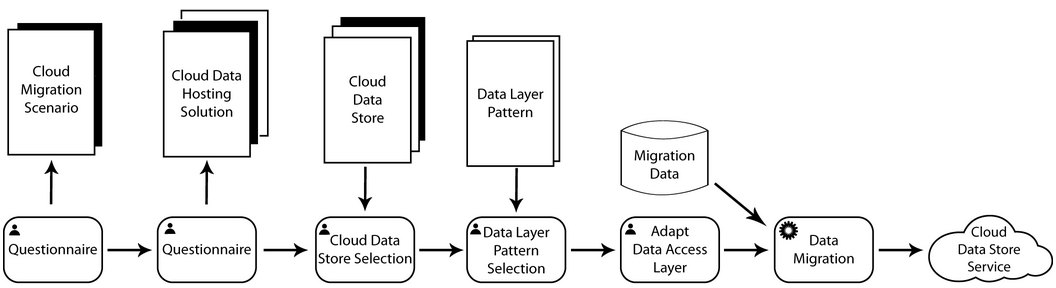
\includegraphics[clip, scale=0.4]{./gfx/clouddatamigrationtool.png}
	\caption[Cloud Data Migration Application - Cloud Data Migration Process]{Cloud Data Migration Process \cite{bachmann2012}} 
	\label{fig:cloudmigrateapp}
\end{figure}

In the \term{data layer pattern selection} and \term{adapt data access layer steps}, the user must specify how to connect to the data store his data is migrated to, and provide the necessary information to establish the connection. The extension of ServiceMix-mt for enabling Cloud data access support allows the user to select this prototype for transparently access the migrated data. 

\FloatBarrier
\section{Apache JMeter}
\label{sec:jmeter}  

Apache JMeter is a Java-based application which provides support for load testing and performance measurement \cite{jmeter2013}. It provides support for different communication protocols, e.g. \ac{HTTP}, \ac{SOAP}, database via \ac{JDBC}, etc. A multi-protocol support enables the application to be used for testing different layers of an application, e.g. presentation layer, and database layer. Furthermore, the user can configure in JMeter different load parameters, e.g. number of threads, iterations, etc., in order to build a heavy load simulation to run on the backend server. Simulation results are presented in structured formats for posterior analysis. 

In this diploma thesis we provide an evaluation of the behavior of the final prototype. Due to the \ac{JDBC} functionality supported by JMeter, we use it to generate the load test cases which are run on ServiceMix-mt.

\FloatBarrier

\chapter{Related Works}
\label{chap:relatedworks}

In this chapter we provide a general overview on the different approaches that are taken into account in order to provide a reliable, secure, and transparent communication between on-premise application's layers and off-premise Cloud data stores. Furthermore, we discuss about the needed adaptations different authors specify that the on-premise application's layers must address when migrating their underlying layers to a Cloud infrastructure. We compare it to the ones we transparently support in our approach, and the ones the user should consider. We finally mention the improvements we need to perform to the original prototype ServiceMix-mt, and continue our discussion dividing it into the two main \ac{DBMS} available nowadays in the market: \ac{SQL} and \ac{NoSQL} databases.

%% non functional data layer patterns paper: make a big emphasis on the proxy approach. It is quite similar to our approach, because it allows horizontal scalability between different target data sources, but there is no need of abstracting the proxy from the database layer. esb's are horizontally scalable and can form a esb cluster, as described in the esb part in fundamentals. we can have in our approach a bottleneck when using one instance of the esb. furthermore, their proxy approach assumes that the database layer is in the private cloud, while in ours the database layer can reside either on or off premise.
A migration process of the Database Layer of an application to the Cloud may pop up several incompatibilities with the new hosting environment, which need to be addressed prior to the migration decision. Strauch et al. aim to address such incompatibilities by defining a set of \term{Cloud Data Patterns}, which target finding a solution for a challenge related to the data layer of an application in the Cloud for a specific context \cite{strauchABKL2012}. Incompatibilities a user may find when migrating the application's data layer can be on the level of the schema representation, supported set of queries or query language, communication protocol, security, etc. Strauch et al. focus mainly in two non-functional aspects: enabling data store scalability and ensuring data confidentiality \cite{strauchABKL2012}. 

The former deals with maintaining the quality of service levels when the workload increases, for both write and read operations. There are two scalability mechanisms when dealing with data: vertical and horizontal scalability. A vertical scalable system can be obtained by introducing more powerful hardware, or moving to a more powerful database system, while a horizontal scalable system deals with splitting data into groups which are stored in different partitions or different database systems, also known as \term{sharding}. Due to the absence of support for accessing a \term{sharded database} between different database systems, the concepts of a database proxy and sharding-based router are introduced. In this first approach, a proxy component is locally added below each data access layer \cite{strauchABKL2012}. A proxy below each data access layer instead of a common proxy on top of the database layer dismisses a common point of failure when accessing the data. In the second approach, a local sharding-based router is added below each of the data access layer. A sharded-based router contains the needed knowledge about the location of the \term{sharded databases}. In our approach, we don't only partially follow both of the concepts, but integrate them in a single component. We consider a sharded-based router as a proxy with routing capabilities. Therefore, as it is discussed in Chapter \ref{chap:design}, enhancing an \ac{ESB} with the required \term{sharded databases} knowledge and with standardized communication protocols, it allows us to utilize it as a sharded-based router, and as a proxy. Furthermore, the single point of failure avoidance can be ensured by increasing the number of \ac{ESB} instances and balancing the load between them. As discussed before, we do not fully comply with this approach. The development of a proxy or sharded-based router component below each data access layer forces each application to deploy at least one proxy or sharded-router instance in their system. In our approach we propose the utilization of our prototype as a shared transparent Cloud data access layer by connecting to a data access endpoint which supports a specific \ac{DBMS} multi-tenant aware communication protocol (e.g. MySQL or PostgreSQL). For this purpose, we propose the concept of a lightweight Data Layer, where the adaptations to its sublayers are minimized, e.g. modification of data access host, port, etc. The data access endpoint acts as a database protocol-aware proxy, forwarding the requests to the \ac{NMR} of the \ac{ESB}. We enhance the Myosotis Tungsten Connector and provide access control, caching functionality, and full integration in the \ac{ESB} \ac{OSGi} container, and with the \ac{NMR} \cite{tungstenwiki}.

%% Data confidentiality between the on premise app layers and the migration layers and how can we still ensure data confidentiality: mention the 5 patterns that are in steve's article. Mention that this article gives a deep focus on security patterns rather than technical information regarding the router between the data stores. we do not implement automatic data filtering for confidentiality. the user is the one who decides which data goes off premise and which data stays in premise. we provide support for off premise and on the on premise data. however, this can be reached in our esb but requires user customization, in order to be able to filter data per user and to route it to the appropriate data store.

Ensuring data confidentiality is presented in \cite{strauch2012}. Their work deals with critical data management between on-premise and off-premise data stores, and categorizes data into different confidentiality levels to prevent data disclosures. The former is achieved by aggregating information which categorizes data into different categories and confidentiality levels. The latter deals with keeping confidential data on-premise. With data filtering, pseudonymization, and anonymization, data is either prevented from being externally routed, or secured when routed to a public Cloud \cite{strauch2012}. The pseudonymization technique provides to the exterior a masked version of the data while maintaining its relation with the original data, and the anonymization provides to the exterior a reduced version of the data. In this diploma thesis' approach, we assume that the application's owner has decided on which data should be and cannot be migrated, and that the business layer is hosted on-premise. Therefore, there is no data processing in a public Cloud environment. Our final prototype provides confidentiality between different tenants of the system by injecting tenant information  in our messages and providing tenant-aware routing, and different multi-tenant aware endpoints. We do not need to provide support for pseudonymization or anonymization techniques, in contrast to \cite{strauch2012}.

%% table of what do i have to do when migrating app or app components to the cloud. this is from the book chapter of vasilios and steve. comment here what ive written in the comments
Replacement of components which build an application with Cloud offerings leads the developers to face an application's adaptation process. For example, migrating a local database to a private Cloud or to a public Cloud, or sharding a database between on-premise and off-premise data stores forming a single data store system, can not be accessible without adapting the non-migrated application's layers to the new storage system. Andrikopoulos et al. identify the needed adaptations actions when migrating a data layer to the Cloud \cite{andrikopoulos2013}: address reconfiguration, patterns realization, incompatibilities resolution, query transformation, and interaction with data store allowance. Our main goal in our final prototype is to minimize the number of adaptations the user must perform when migrating application's data to a Cloud data store. The adaptations of the \ac{ESB} must encompass the described adaptations in a transparent way to the user, in order to internally support in our prototype compatibility between the application and the different data stores, and lower the adaptation operations number at the application's side, e.g. only address reconfiguration. 

%% speak a little bit about federated databases
%% have taken notes in the paper. the main thing to say here is the main difference between a federated database system and our approach. Our approach works more or less than a federated database system, but more like a federated server, where transparent access to backend datasources is provided. joins are out of the scope of the thesis. indicate that one main component in a federated dbs is the transformer, in our case between sql databases, and between nosql databases, but this is out of scope of this thesis. 
%% mediator in page 37 of the book principles of distributed database systems
Federated Database Systems are a type of \ac{MDBS} that allow accessing and storing data which is stored in different and noncontiguous databases through a single interface. Sheth and Larson define them as a collection of cooperating but autonomous component database systems, which can be integrated to various degrees, and can be accessed by a software which controls and coordinates the manipulation of the database systems which conforming the federated database system. This distributed database model allows users to access and store data among different database systems, which can be located in different continents, without dealing with multiple connections to the different database systems, query and data transformation, address adaptation, etc. \ac{MDBS} are accessed through a single endpoint which provides a single logical view of the \ac{MDBS}, and users can access the different \ac{DBMS} which form the \ac{MDBS} (see Figure \ref{fig:multidatabasesystem}). 

\begin{figure}[htb]
	\centering
		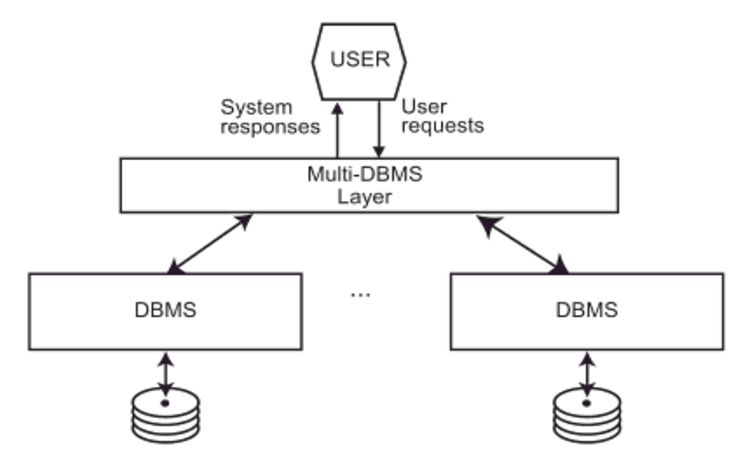
\includegraphics[clip, scale=0.6]{./gfx/multidatabasesystem.pdf}
	\caption[Multidatabase System Components]{Components in a multidatabase system \cite{ddbsozsu}}
	\label{fig:multidatabasesystem}
\end{figure}

A popular implementation architecture for a \ac{MDBS} is the mediator/wrapper approach \cite{ddbsozsu}. Mediators exploits knowledge to create information for upper layers, while wrappers provide mapping between different views, e.g. relational vs. object-oriented views. We can consider our approach as a \ac{MDBS} with some modifications and less functionalities. In the first place, using the \ac{ESB} as a single entrance point to the data system while managing different backend autonomous Cloud or traditional data stores comply with the main concept of a \ac{MDBS}. Furthermore, Cloud data store providers may implement the same distributed database model, whereby we could find two logical levels for accessing the physical data. However, we do not accurately follow the mediator/wrapper approach. In our approach we exploit data provided by the tenant during the migration decision and process, by providing an interface to register the backend data store/s information in our system, for future routing purposes. Furthermore, compatibility information is registered in order to apply the needed query or data transformation between data stores. However, the transformation is out of the scope of this diploma thesis, and the support of table joins between databases located in different Cloud data stores are out of scope as well.
%%tenant isolation approach in muhler versus tenant and user isolation approach in this work. explain the granularity of tenant and users, one tenant may want to migrate his database to a data store, but in this case one database can have one or more users. it is not like in muhlers approach where tenants are considered applications accessing the esb. 

As described in the previous chapter, multi-tenancy is one of the main requirements in a Cloud environment. Muhler, Essl, and Gomez provide an extended version of ServiceMix 4.3, which supports multi-tenancy at two different levels: communication, and administration and management \cite{Muhler2012}, \cite{Essl2011}, \cite{gomez2012}. However, their prototype supports tenant isolation at the level of tenants. A \ac{DBMS}, e.g. MySQL, by default provides access to one default user and supports multiple users creation \cite{mysqlmanual}. Therefore, in our approach we must not only consider isolation at the tenant level, but also at the user level. We assume that the tenant is the default user which migrates his data store to a Cloud environment, but the migrated data store may contain one or more users. In our prototype we ensure tenant and user isolation at both communication, and administration and management levels.

%% caching mechanism used in our approach, explaining the two levels of caching that we use. compare it to the actual mysql proxy and to the databases architectures in the cloudcomputingdatabaseapps paper, say that caching is not discussed in their approach. caching applies for both mysql and nosql. drivers provided by the different vendors do not provide caching functionality. caching functionality must be trated in the application or in the server. caching is good not only for performance, but also to give the possibility to reduce costs in the tenants data stores in the cloud. most of the providers dont only charge per storage size, but also per calls to their api
%%mention the paper
%% put examples on amazon pricing : Micro DB Instance	$0.025 Small DB Instance	$0.090 Medium DB Instance	$0.180 Large DB Instance	$0.365 Extra Large DB Instance	$0.730 this are prices of usage per hour
%% amazon dynamo db: Write Throughput: $0.01 per hour for every 10 units of Write Capacity - Read Throughput: $0.01 per hour for every 50 units of Read Capacity
%% google cloud storage: (per 1,000 requests/month) PUT, POST, GET bucket**, GET service** Requests $0.01 - GET, HEAD Requests (per 10,000 requests/month) $0.01 - DELETE Requests free
Over the past decades, caching has become the key technology in bridging the performance gap across memory hierarchies via temporal or spatial localities; in particular, the effect is prominent in disk storage systems \cite{cashing2012}. Han et al. investigate how cost efficiency in a Cloud environment can be achieved, specially in applications which require a high I/O activities number, and present a CaaS (cache-as-a-service) model. Cloud providers offering data storage solutions present pricing models based on the storage size, usage per time, or number of requests. Amazon RDS costs \$0.025 per hour for a Micro DB Instance usage  \cite{amazonrds}, while Amazon DynamoDB \$0.01 per hour for every 50 units of read capacity \cite{amazondynamodb}, and Google Cloud Storage \$0.01 per 1000 PUT, POST, GET requests per month \cite{googlecloudstorage}. An I/O-intensive application whose database is hosted in the Cloud may produce a significant economic cost. The cost of continuously retrieving data from the Cloud data store, when existing temporal proximity between the data accessed, can be considered unnecessary, and reducible. Furthermore, the application's overall performance can be reduced due to the network latency and, in the scope of this work, the use of an \ac{ESB} to access the Cloud data store. In this diploma thesis we do not provide cashing as a service, but include cashing support to the sharded-based router pattern described in \cite{strauchABKL2012}. Uralov enhaces ServiceMix-mt with cashing support for dynamic discovery and selection of Cloud data hosting solutions \cite{Uralov2012}. However, we must adapt and extend it due to the lack of support of functionalities we require and the lack of full \ac{OSGi} compliance. 

\section{SQL Support Architectural Overview}
\label{sec:designsql}

In this section we provide an overview of a preliminary, and final architectural approaches designed in this diploma thesis, in order to support a transparent data access to backend \ac{SQL} databases. We first expose the integration approaches we should consider, and the main problems found when implementing the first approach which led us to design a second architectural approach. 


\subsection{Integration}

%integration of osgi and jbi in terms of messaging
%integration of osgi and jbi in terms of containers and libraries
%explain why we have two approaches
%jbi components offered in servicmix are deployed as osgi bundles
% jbi components offered in servicemix-mt are deployed as jbi component, and internally wrapped into an osgi bundle
% may have to put a figure of the contents in both of the packages so that we can see. It is all about the meta inf library where the bundle manifest info is exposed
As described in Chapter \ref{chap:spec}, we build the new components in ServiceMix-mt following the \ac{OSGi} compliance. However, these must interact with components which follow the \ac{JBI} specification. The integration between components built for different containers in ServiceMix-mt must be done at two levels: messaging, and resources sharing. The ServiceMix-mt \ac{NMR} \ac{API} \ac{OSGi} bundle exposes a set of operations for sending messages through the \ac{NMR} to a specified target endpoint. Hereby we can perform message exchanges between endpoints configured on \ac{OSGi} bundles and endpoints configured on \ac{JBI} components, and provide communication support between components hosted in the two containers. 

\begin{figure}[htb]
	\centering
		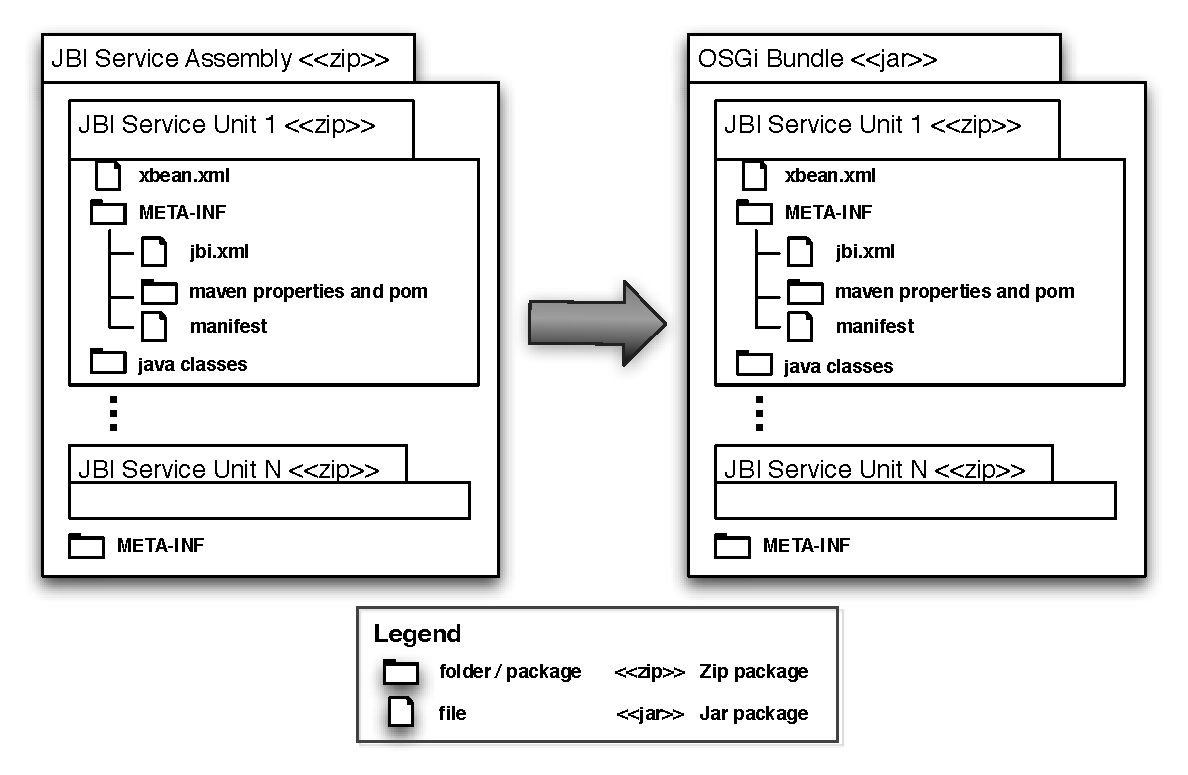
\includegraphics[clip, scale=0.5]{./gfx/osgibundlepackage.pdf}
	\caption[JBI to OSGi repackaging]{ServiceMix 4.x repackaging mechanism for deploying \ac{JBI} components in \ac{OSGi} container.}
	\label{fig:jbitoosgipackage}
\end{figure}

The resources sharing integration level refers to the deployment of \ac{JBI} components in the \ac{OSGi} container, and the utilization of packages exposed by \ac{OSGi} bundles in the \ac{OSGi} container in a loosely coupled manner. The former is part of the integration between containers provided in ServiceMix 4.x versions and described in Figure \ref{fig:jbitoosgipackage}. The deployment mechanism of a \ac{JBI} \ac{SA} into an \ac{OSGi} container is simple: repackaging of the \ac{SA} as a JAR. However, this cannot be consider a full integration in the \ac{OSGi} container. \ac{OSGi} bundles contain in their \term{META-INF} folder one fundamental file for the \ac{OSGi} kernel: the \term{manifest} file. This contains a description of the bundle, the packages it imports, and exports. Imported packages can be either statically stored in the bundle or imported from third party bundles, and exported packages are the ones which exposed to third party bundles. These can be imported with an internal class loading mechanisms developed in the \ac{OSGi} container. The repackaging of the \ac{SA} into a JAR, as it is shown in Figure \ref{fig:jbitoosgipackage}, contains the \term{META-INF} folder, and the \term{manifest} file. However, the latter only contains information about the author, date of creation, but it does not contain information related to the exported packages, and the needed packages to be imported. This \term{manifest} file describes the \ac{SA}, and not the \ac{SU}s. Java classes and package importing description are contained in the \ac{SU} package, and not in the \ac{SA} package. Therefore, the \ac{OSGi} container cannot register in its registry the packages it exports as a service, and cannot load the imported packages to the bundle context. This fact forces us to statically include in the \ac{SA}, and the \ac{SU} the packages which are referenced in each \ac{SU}, and leads to scalability constraints with the tenant-aware deployment process of the system.

ServiceMix 4.x versions are shipped with different \ac{JBI} \ac{BC}s packed as an \ac{OSGi} bundle. However, they are deployed as \ac{OSGi} bundles, and not as \ac{SA}s, in order to enable loose coupling and package sharing between components in the \ac{OSGi} container. ServiceMix-mt allows the deployment of the \ac{JBI} \ac{BC}s, but deployment of \ac{JBI} \ac{BC}s as OSGi bundles is not supported in the JBIMulti2 application. This lack of support forces us to design a second architectural approach, as described in the following sections.

\FloatBarrier

\subsection{Approach 1}

\ac{SQL} database systems provide access to their databases through an endpoint, which is represented as an URL. The native driver used in the data access layer of an application connects to the endpoint, authenticates, sends the query, and reads the response. Therefore, we must support in our system the same operational steps. As discussed in this diploma thesis, the communication protocol varies between different vendors. In this diploma thesis we provide support for incoming MySQL messages. Tenants must access our system through a single physical endpoint. This endpoint is provided by a MySQL proxy which is enriched with authentication, cashing, marshaling, and demarshaling operations. As shown in Figure \ref{fig:designsqlapp1}, the MySQL Proxy Bundle implements the MySQL server operations which are related with the client/server communication protocol. In Figure \ref{fig:designsqlapp1} we specify a server running on port 3306. However, this value can be configured before the deployment of the \ac{OSGi} component. This component is built as an \ac{OSGi} bundle and its packages are exported as services in the \ac{OSGi} container. It interacts with three different components in the system: the \ac{NMR} \ac{API}, the Cache, and the Service Registry. 

Cashing mechanisms are implemented in both the Registry-Cache, and the MySQL Proxy Bundle. The former provides an \ac{API} for creating cache instances, and for persisting and retrieving data. We create a separate cache instance for the \ac{SQL} support due to the need of a custom key creation mechanism which may not coexist in a shared cache between different bundles, as well as the needed isolation of sensible tenant configuration information from third party bundles. The system provides a set of operations which ease the creation of multi-tenant aware keys for persisting frontend authentication data, and queries results form the backend database systems. 

The \ac{NMR} \ac{API} is shipped in ServiceMix as an \ac{OSGi} bundle which exports its \ac{API} as an \ac{OSGi} service. The set of operations included in its \ac{API} allows \ac{OSGi} bundles to create, send, and receive message exchanges to \ac{JBI} endpoints (see Figure \ref{fig:designsqlapp1}).  Before creating the message exchange, the MySQL Proxy Bundle must build dynamically the target endpoint's URL by injecting the tenant context information, and service and endpoint name.

\begin{figure}[htb]
	\centering
		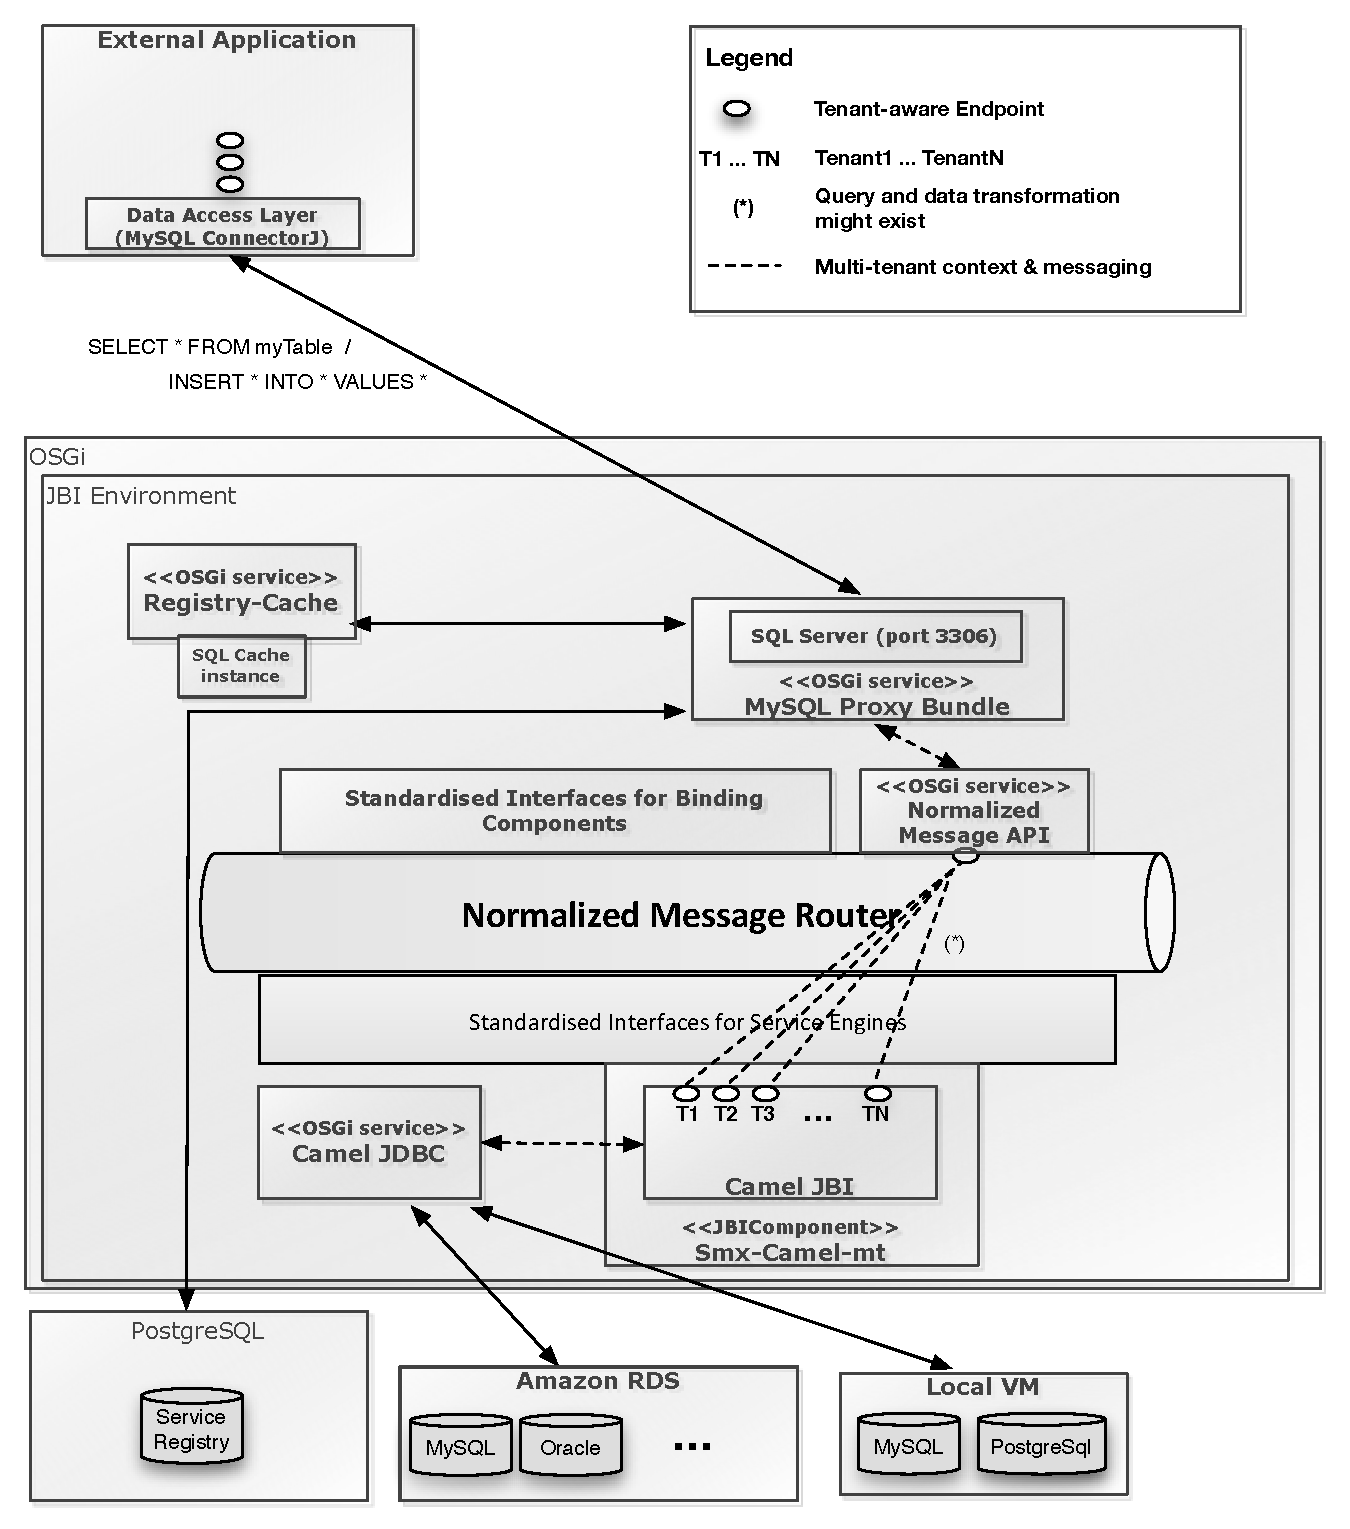
\includegraphics[clip, scale=0.6]{./gfx/sqlApproach/sqlApproachv2_doc.pdf}
	\caption[SQL Support Approach 1]{Architectural overview of the design approach one to support the MySQL communication protocol and routing to backend \ac{SQL} databases.}
	\label{fig:designsqlapp1}
\end{figure}

Apache Camel provides a set of components which integrate most of the communication technologies available in the market. Moreover, it provides an archetype for creating custom components we use in this diploma thesis. ServiceMix provides a Camel \ac{JBI} \ac{BC} which integrates the \ac{JBI} container with the camel router. Muhler extends this component in ServiceMix-mt and enriches it with multi-tenancy awareness. However, the supported multi-tenancy is at the level of tenants, and not at the level of tenant's users. We extend this component and provide user and tenant isolation between endpoints, by injecting the tenant and user UUID in the endpoint's URI (see Listing \ref{lst:endpointuri}). 

%%%%%%%%%%%%%%%%%%%%%%%%%%%%%
\lstinputlisting[float=htb,label={lst:endpointuri},caption={[Tenant-aware Endpoint Configuration]Extended Tenant-aware endpoint URI in extended Backus-Naur Form (EBNF) \cite{Muhler2012}.},style=ebnf]{./gfx/endpointconfiguration.txt}
%%%%%%%%%%%%%%%%%%%%%%%%%%%%%

With multi-tenancy at the tenant and user level, each user can deploy one \ac{JBI} tenant-aware endpoint in the ServiceMix-Camel-mt \ac{SE}. The routes deployed from each tenant-aware endpoint are performed under a different context, and an instance of the targeted component in the route is created. Therefore, with this approach we provide multi-tenancy at the messaging, endpoint, and routing and component context levels. 

Due to the lack of \ac{JDBC} support in ServiceMix for creating provider endpoints, we develop a custom camel component, and enrich it with \ac{JDBC} support for three database systems: MySQL, Oracle, and PostgreSQL. This component is extensible to more database systems when including its native driver, and is build as an \ac{OSGi} bundle and its packages are exported as an \ac{OSGi} service. Messages received from the \ac{NMR} are demarshaled to the backend database system communication protocol, and the response marshaled, correlated, and sent back to the MySQL Proxy Bundle. The demarshalers in this bundle provide the necessary support for transforming the \ac{NMF} response to a MySQL message.

As described in the previous section, ServiceMix-mt provides \ac{JBI} and \ac{OSGi} support and integration, but with some constraints. \ac{JBI} components cannot import packages from \ac{OSGi} bundles exporting its packages. The Servicemix-Camel-mt \ac{SE} provides integration with the camel router for a set of camel components. The camel manual specifies the need for adding statically the custom component packages in the \ac{JBI} \ac{SU} which contains the route definition. Therefore, this leads us to scalability problems in each of the \ac{SA} deployed by the tenants. The \ac{SA} size increases with the new supported database systems, and forces to redeploy all the \ac{SU}s containing the custom camel component when it is modified. This leads to management, storage capacity, and network capacity inconveniences. Hence, we provide a second, and final approach which is very similar to this one, but utilizing the ServiceMix-camel component deployed as \ac{OSGi} bundle. 

\FloatBarrier

\subsection{Approach 2}

In this second architectural design approach we address the scalability problems caused by the \ac{JBI} package dependencies in the \ac{SU}s described in the previous section. This approach is similar to the first one presented, and its main difference relies on the routing from the tenant-aware \ac{JBI} endpoints to the custom camel component \term{cdasmixjdbc} (see Figures \ref{fig:designsqlapp2} and \ref{fig:designsqlapp1}). The functionalities and operations in the MySQL proxy bundle do not differ with the previous approach.
 
\begin{figure}[htb]
	\centering
		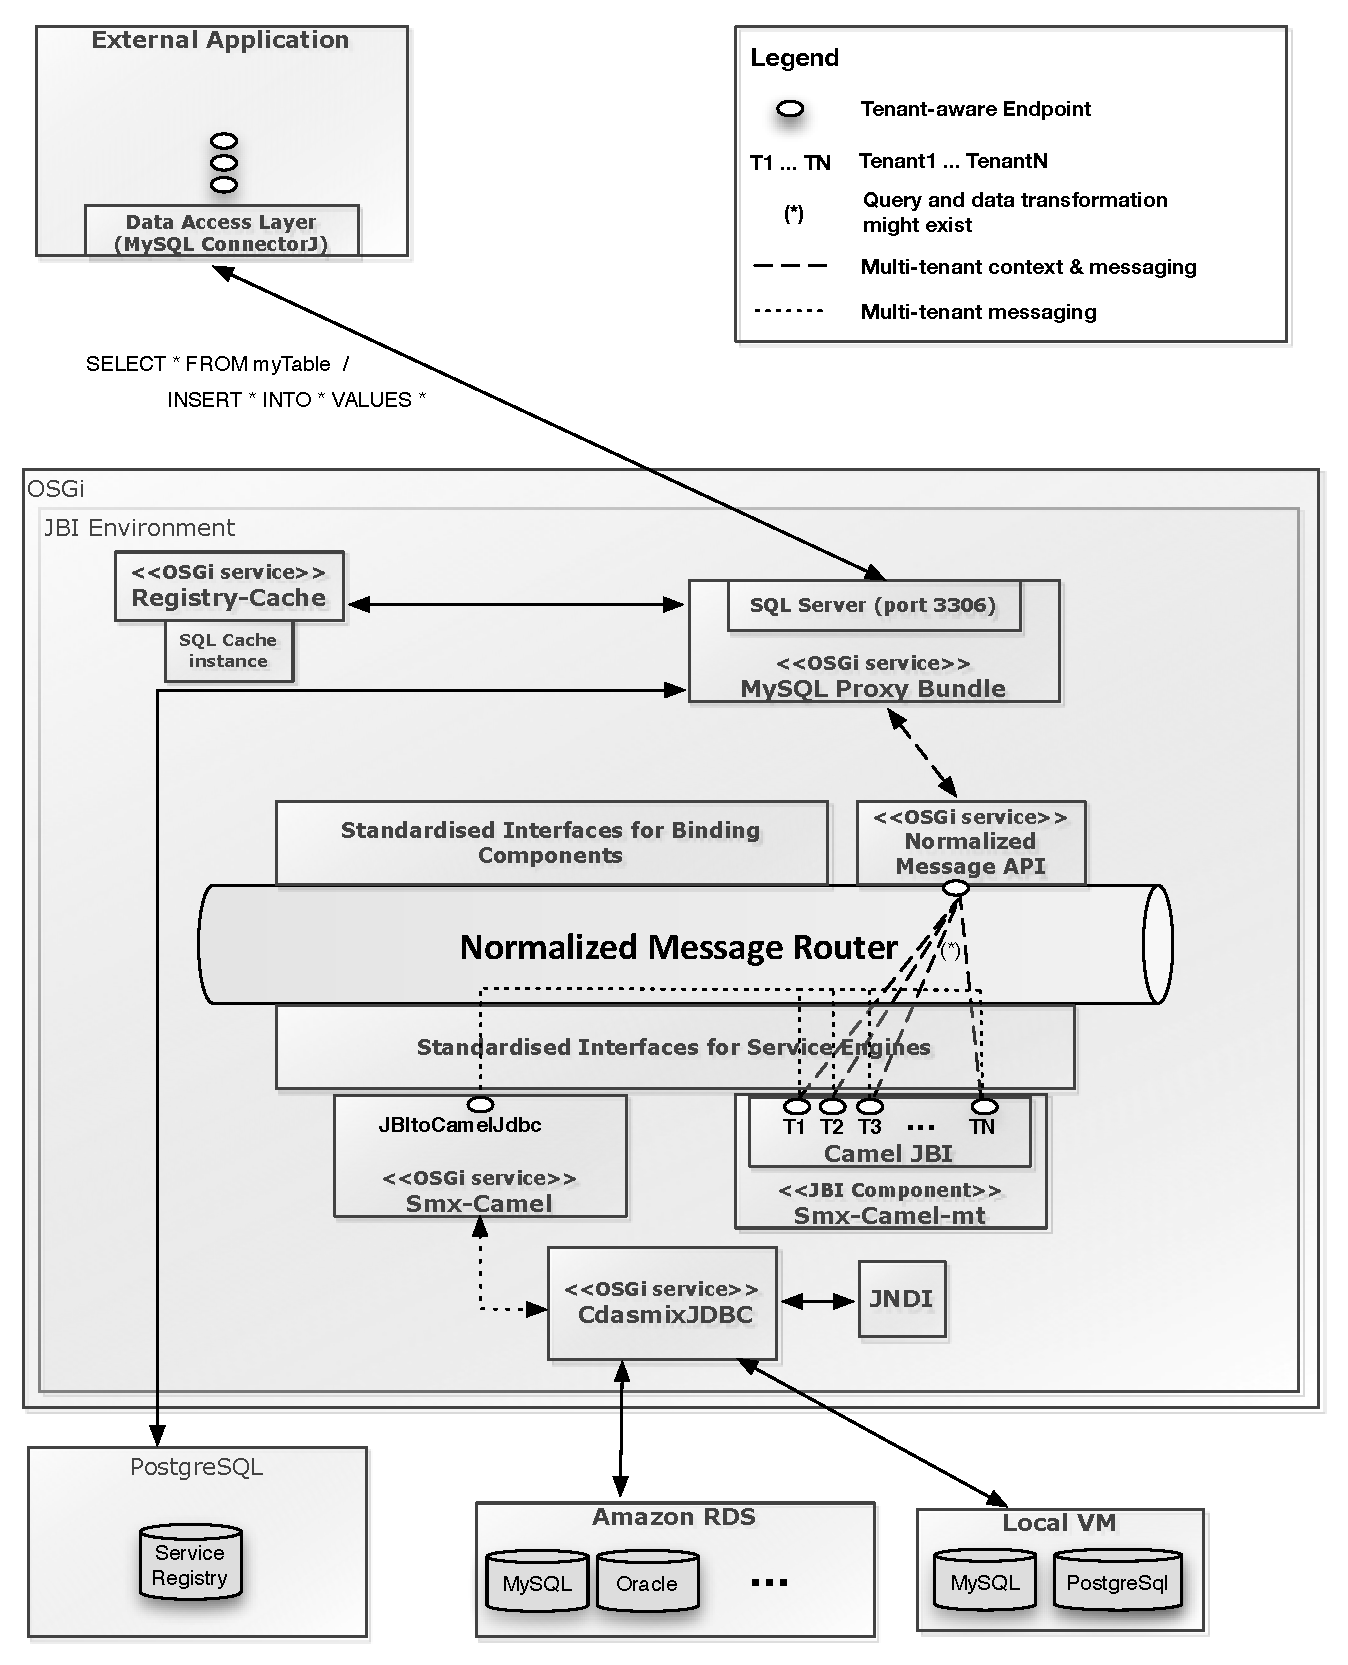
\includegraphics[clip, scale=0.6]{./gfx/sqlApproach/sqlApproachv3_doc.pdf}
	\caption[SQL Support Approach 2]{Architectural overview of the design approach two to support the MySQL communication protocol and routing to backend \ac{SQL} databases.}
	\label{fig:designsqlapp2}
\end{figure}

The message is routed from the MySQL proxy bundle to the tenant-aware \ac{JBI} endpoint deployed in ServiceMix-camel-mt. The multi-tenant message processor instance in ServiceMix-camel-mt routes the message to the \term{JBItoCamelJdbc} endpoint. 

As discussed before, the \ac{JBI} \ac{BC}s deployed in ServiceMix are \ac{OSGi} friendly. This means that the \ac{OSGi} contains a valid manifest file where the description of the bundle, import packages, and export packages are specified. \ac{SU}s deployed on this component are able to reference other \ac{OSGi} packages exposed as a service in the \ac{OSGi} service registry. We provide a single endpoint deployed in the ServiceMix-Camel component where the requests are sent to: the \term{JBItoCamelJdbc} endpoint. When the \term{JBItoCamelJdbc} endpoint is deployed on the ServiceMix-Camel \ac{OSGi} bundle, this searchs in the \ac{OSGi} container for the \term{CdasmixJDBC} component, and creates an instance of the component. Messages routed to the \term{JBItoCamelJdbc} endpoint are then forwarded to the \term{CdasmixJDBC} component, which selects the appropriate \ac{JDBC} native driver, creates a connection, demarshals the request, and forwards the request to the backend Cloud data store server. The connection is established after creating an instance of a \term{DataSource}, which is saved in the \ac{JNDI} registry for future connections, in order to avoid the creation of more than one \term{DataSource} instance per user per backend Cloud data store.

Responses retrieved from the backend Cloud data store are correlated with the initial request and routed back to the MySQL proxy bundle, which demarshals the retrieved data and sends it as a binary \ac{TCP} stream.

In this approach a new instance of the \term{cdasmixjdbc} is not created per tenant endpoint, but is shared between the tenants. Therefore, we cannot ensure an independent component context at the provider endpoint. However, messages contain the tenant information, and the \term{cdasmixjdbc} component interacts with the backend database system establishing separate \ac{JDBC} connections per request. Full multi-tenancy, at the levels of component creation, and endpoint level is not ensured, but it is ensured at the messaging, and context levels. Although full multi-tenancy is not supported, we avoid the deployment of \ac{SU}s which contain the \term{CdasmixJDBC} component in it, and whose size increase may lead to scalability problems in the system. Furthermore, we prevent the deployment of the same component n times, for the n multi-tenant aware endpoints, and prevent future management problems when modifying or upgrading the \term{CdasmixJDBC} component. 

\FloatBarrier



\section{NoSQL Databases}
\label{sec:fundamentalsnosqldb}  

\ac{RDBMS}s ensure data persistency over time and provide a wide set of features. However, the functionalities supported require a complexity, which is sometimes not needed for some applications, and harms important requirements in Web applications or in \ac{SOA} based applications, e.g. throughput. \ac{NoSQL} data stores aim to improve the efficiency of large amount of data storage while reducing its management cost \cite{nosqlcomputerworld}. NoSQL databases are designed to support horizontal scalability without relying on the highly available hardware \cite{strauchnosql}. In a Cloud storage environment where the user sees the available computing and storage resources as unlimited, a \ac{NoSQL} support in a Cloud storage environment might be adequate.

\ac{NoSQL} \ac{DBS} operate as a schema-less storage system, allowing the user to access, modify or freely insert his data without having to make first changes in the data structure \cite{nosql2012}. Cloud providers provide the users with an \ac{API} for accessing, modifying, and inserting data into his isolated container. For example, a user's Amazon Dynamo DB table and item can be accessed by its RESTful \ac{API}, or by installing at the user's side application the Amazon Web Services SDK \cite{amazondynamodb}. Furthermore, it provides the users through its Web-based management console the available management operations. 

Due to the growth of the \ac{NoSQL} support along different Cloud vendors, in this diploma thesis we provide a multi-tenant and transparent communication support for \ac{NoSQL} backend data stores in different Cloud providers. In the following sections we introduce the categorization of the different \ac{NoSQL} databases we aim to support in this diploma thesis, mentioning and giving examples of Cloud data stores available nowadays in the market.

\subsection{Key-value Databases}

In a key-value datastore elements are uniquely identified by an id, which the data store does not take into account its type, and are simply stored as a \ac{BLOB} . A user can get the value for the key, put a value for the key, or delete a key from the data store \cite{nosql2012}. Its storage model can be compared to a map/dictionary \cite{strauchnosql}. Products offering this data storage model in a Cloud infrastructure are Amazon DynamoDB \cite{amazondynamodb}, Google Cloud Storage \cite{googlecloudstorage}, Amazon SimpleDB  \cite{amazonsimpledb} , Amazon S3 \cite{amazons3}, etc. In this diploma thesis we mainly focus on the following key-value data stores: DynamoDB, and Google Cloud Storage.

Amazon DynamoDB's data model includes the following concepts: tables, items, and attributes \cite{amazondynamodb}. The attributes are a key-value, where the value is binary data. Attributes are stored in items, and these are stored in tables. Items stored in a table can be retrieved by referencing its unique id. The number of attributes is not limited by Amazon, but each item must have a maximum size of 64 KB. Accessing stored data in this data store can be mainly done in two ways: using the functionalities provided by the AWS SDK, or using the Cloud storage RESTful \ac{API}. 

Google Cloud Storage's data model includes the following concepts: buckets and objects \cite{googlecloudstorage}. Buckets contain on or more objects. The objects are identified within a bucket with its unique id. Users can perform I/O operations on both buckets and objects. For this purpose, Google Cloud storage provides RESTful \ac{API}.

In this diploma thesis we use an \ac{ESB} for accessing transparently tenant's databases migrated to the Cloud. Servicemix-mt provides multi-tenant \ac{HTTP} support \cite{gomez2012}. Therefore, we reuse and extend the multi-tenant \ac{HTTP} \ac{BC} in order to provide dynamic routing between the different data stores.

\subsection{Document Databases}

Document databases can be considered as a next step in improving the key-value storage model. In this storage model, documents are stored in the value part of the key-value store, making the value content examinable \cite{nosql2012}. Documents with different schemas are supported in the same collection, and can be referenced by the collection's key or by the document's attributes. One of the main difference in the attributes specification regarding \ac{RDBMS} is that in document stores document's attributes cannot be null. When there is an attribute without value, the attribute does not exist in the document's schema. Products implementing this data storage model are Apache CouchDB, MongoDB, etc. \cite{couchdb} \cite{mongodb}.

Mongo DB defines two storage structures: collections and documents \cite{mongodb}. A specific database contains one or more collections identified by its unique id. A specific collection stores one or more documents. Collections and documents stored in a database can be accessed, inserted and modified using the RESTful \ac{API} supported by the database system.

Apache CouchDB defines two storage structures: databases and documents. Data stored in CouchDB are \ac{JSON} documents. The main difference between this two described databases is that MongoDB implements a two step access to the documents: database, collection, and document. Apache CouchDB provides a RESTful \ac{API} for I/O operations.

This databases are not offered by Cloud providers like Amazon or Google, but as a software which can be deployed in user instances, e.g. Amazon EC2 AMI \cite{amazonec2}. 

\subsection{Column-family Stores}

One of the most known Column-family data stores is Cassandra. Column-family data stores store data in column families (groups of related columns which are often accessed together) as rows that have many columns associated with a row key \cite{nosql2012}. This approach allows to store and process data by column instead of by row, providing a higher performance when accessing large amount of data, e.g. allowing the application to access common accessed information in less time.

Cassandra has as its smallest unit of storage the column, which consists of a timestamp and a name-value pair where the name acts as a key \cite{nosql2012}. As in the relational model, a set of columns form up a row, which is identified by a key. A column family is a collection of similar rows. The main difference with the relational model is that each of the rows must not have the same columns, allowing the designer and the application consuming large amounts of data to customize the columns in each row, and the rows in each column family.

Cassandra is not shipped with a RESTful API for I/O operations. However, there are several open-source services layers for Cassandra, e.g. Virgil \cite{virgil}.

\FloatBarrier

\clearpage  
\section{Specification}
\label{sec:evaluationspecification}



\subsection{Evaluation Requirements}
\label{sec:evalrequirements}

% different message size, reduce loose couple being able to specify different types of messages
% invoke the endpoints with concurrent users and invoke endpoints concurrently
% be able to set the number of concurrent users and concurrent endpoints to invoke at the same time
% include multi-tenancy awareness in the benchmark for the different scenarios
% structured data as the output for analysis, for throughput and response time for the different messages requests for the different endpoints
% has to be done on top of the androitbenchmark, so that we can reuse and extend their benchmark
% system measurements of cpu and memory in structured data. also the measurement of the heap size (real memory consumtion) in the process
% monitoring of number of outgoing requests and incoming requests into the backend service, wireshark

In this student thesis we provide a performance analysis on the integration of the multi-tenant aware approaches in ServiceMix and measure the impact on the performance of the extended prototype. For this purpose, we need to fix which measurements we use for the evaluation. The driver should perform the following measurements: response time (measured in milliseconds) and throughput (measured in number of messages sent per second) respect to a backend service, and CPU and memory usage of the system hosting the instance of ServiceMix. The evaluation has to be done in different scenarios, each of them sending different messages number and sizes, for different multi-tenant and non multi-tenant aware endpoint configurations, as described in Table \ref{tab:evaluation} \cite{EvalESB}.

\begin{table}[htbp]
\centering
\begin{tabular}{llll}

	\toprule
	 Number of Endpoints 		& Messages Size	& ServiceMix Instances		& Multi-tenancy awareness 		\\
	 \midrule
	 
	 1 						& 0.5 / 1 KB 		& 1						& mt and non-mt									\\
	  						& 				& 2						& non-mt											\\
	 2 						& 0.5 / 1 KB 		& 1						& mt and non-mt									\\
	  						& 				& 2						& non-mt											\\
	 4 						& 0.5 / 1 KB 		& 1						& mt and non-mt									\\
	  						& 				& 2						& non-mt											\\
	 10 						& 0.5 / 1 KB 		& 1						& mt and non-mt									\\
	  						& 				& 2						& non-mt											\\														
	 
	\bottomrule
\end{tabular}
\caption[ServiceMix evaluation performance scenarios]{Specification of the different scenarios to be evaluated. In both multi-tenant and non multi-tenant aware evaluations, one user per endpoint / tenant is configured. \\ \term{Legend: mt (multi-tenant aware), non-mt (non multi-tenant aware)}}
	\label{tab:evaluation}
\end{table}

AndroitLogic has developed a performance analysis driver which fulfills most of the above requirements in different scenarios \cite{androit2012}. In our evaluation, we extend the Direct Proxy scenario from the AndroitLogic  \ac{ESB} Performance benchmark \cite{androit2012}. However, it doesn't achieve one of the main requirements of this student thesis: multi-tenant aware messaging and concurrent invocation between endpoints. Those two requirements should be included in an extended version of the primitive driver. Furthermore, the extension should be utilized with different \ac{ESB} solutions and must be user-friendly configurable for the different scenarios. The output of the driver measurements should be analyzed, therefore the output data must be in structured format. 

\subsection{Evaluation Overview}
\label{sec:evaluationoverview}

% main picture of the overview of the system for evaluating the esb and explain it with detais of the hardware setup of the vm
% describe a little bit the scenarios that were fixed
% 
In the Section \ref{sec:requirements} we have described the requirements that the evaluation should fulfill and the needed modifications in the utilized benchmark. As exposed in Figure \ref{fig:evaluationoverview}, the evaluation is conformed by three main independent systems. We must ensure, for analyzable purposes, that we approximate as much as possible to a Web service standard real scenario: service requester invokes a backend service and both request and response are routed through the network. In our evaluation we must utilize the \ac{ESB} as a mediator between the service requester and provider. In the first system (VM0), both service requestor and provider are deployed. The communication measurements are taken in two different components: throughput and response time in the AndroitLogic driver, while the number of incoming and outgoing requests, as well as the visualization of the messages, have to be monitored in an independent monitoring component. 

In the second and third systems (VM1 and VM2 respectively) one instance of ServiceMix is deployed for routing the messages between the AndroitLogic driver and the backend service. A monitor component must perform the counting of the incomming and outgoing requests to and from the \ac{ESB}, and a system monitor component should measure the \ac{ESB}'s resources consumption. The connection between the components in VM0 and VM2 is represented with a dashed line, because the VM2 is only use for non multi-tenant aware scenarios. Similarly, we have connected the components in VM0 with the components in VM1 with a continuos line, because this connection is used in both multi-tenant and non multi-tenant aware scenarios. 

The JBIMulti2 application is used for deployment of the \ac{SA}s which pack the endpoint configurations in the \ac{SU}s. However, we do not include the JBIMulti2 application in our overview because we do not evaluate the JBIMulti2 performance, but the multi-tenant and non multi-tenant ServiceMix independently from the JBIMulti2 application.

\begin{figure}[htb]
	\centering
		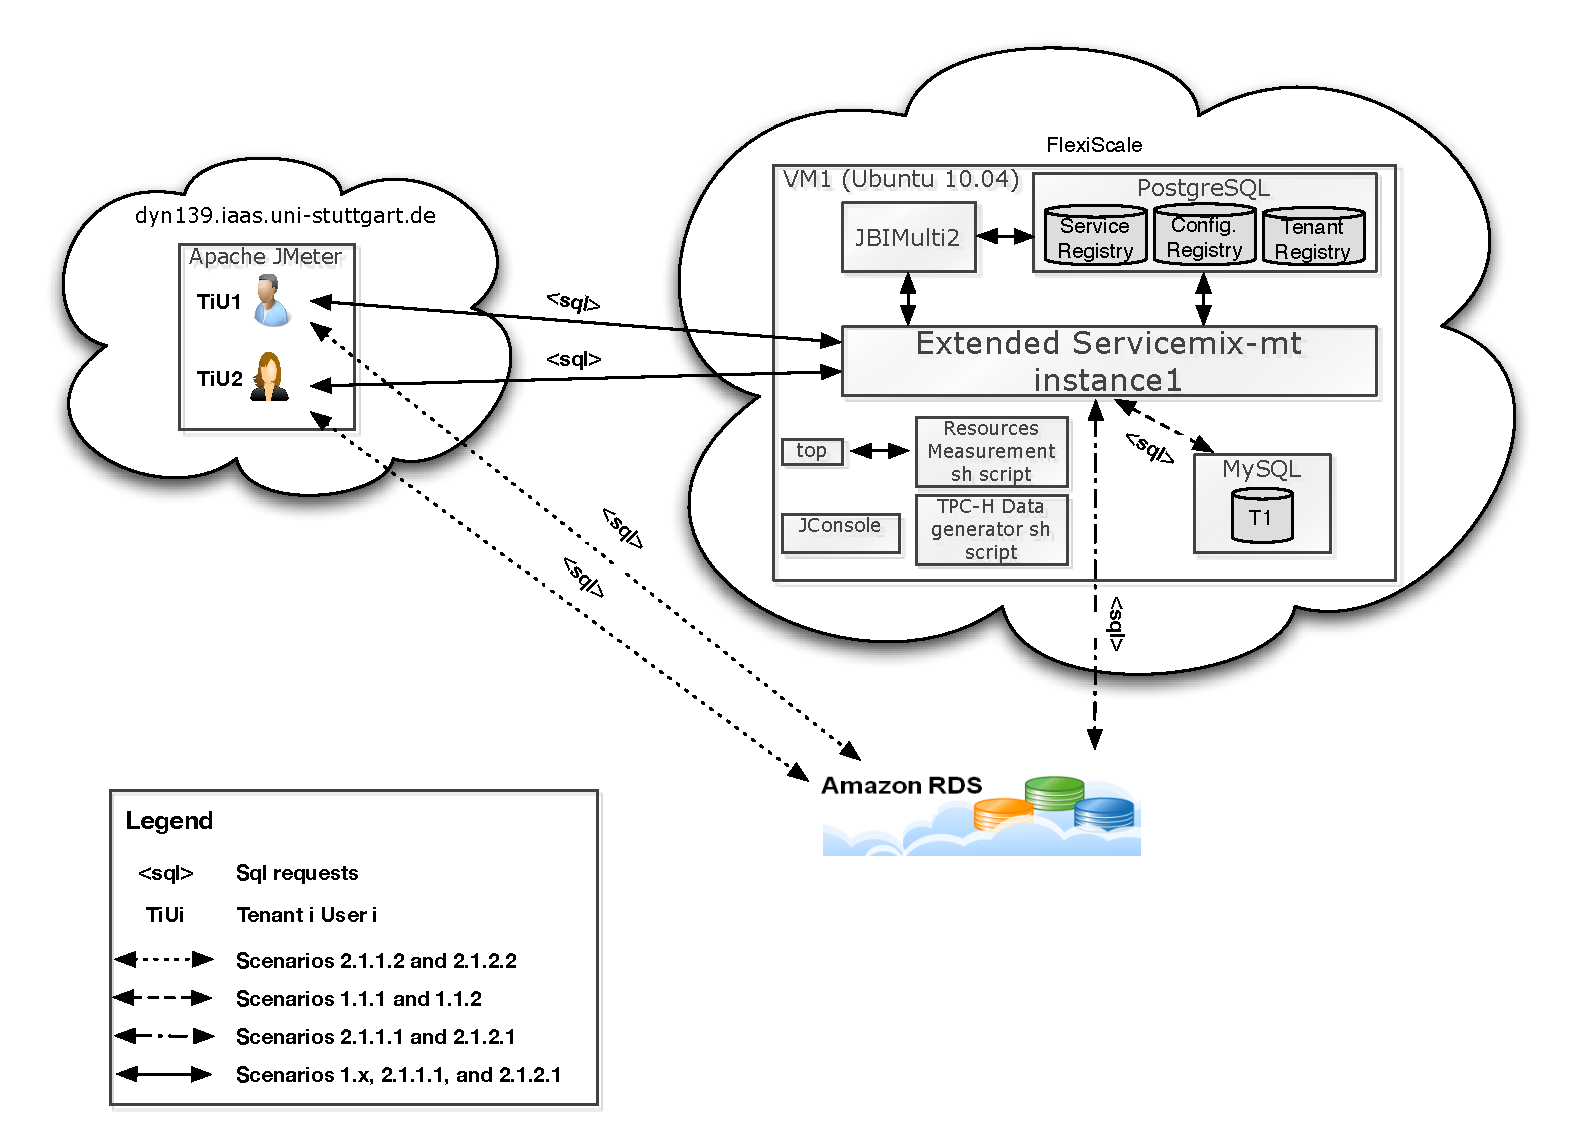
\includegraphics[width=0.7\textwidth, trim=0.0cm 0.0cm 0.0cm 0.0cm, clip]{./gfx/evaluationoverview.pdf}
	\caption[Performance Evaluation Components Overview]{Overview of the components used for the \ac{ESB} performance evaluation. \textbf{Note:} In the evaluation two different monitors are used. For communication the monitoring requires the counting and visualization of the incoming and outgoing requests. For system monitoring, the CPU and Memory usage should be measured.}
	\label{fig:evaluationoverview}
\end{figure}

\FloatBarrier

\FloatBarrier
\section{ESB Performance Evaluation Architecture}
\label{sec:esbevaluationdesign}

% explain the figure
% the evaluation is done for SOAP over HTTP protocols based on a in only message exchange patter, so that we are only masuring how much time does it take to reach the backend service. explain that the dashed lines are because those calls are optional, this means, we divide in to more than one scenario, each scenario testing 1, 2, 4, and 10 endpoints
% for the two instances of servicemix, we provide 10 endpoints in total, and 5in each instance, and the load is divided into the endpoitns. we start with the scenario with 2 endpoints
% explain a little bit the java bench androitlogic driver
% explain that we will use differente messages for the scenarios so that we can decouple them from the scenarios, being able to modify messages independently. results are in a format (I can paste an example of a result from the java benchmark) and then the driver provided by androit to be able to convert it to a csv file
% for concurrent calls between endpoints, we are going to create as many instances of the java benchmark as many endpoints we want to call concurrently by using shell scripting and the & (background task). Explain how many messages we are sending, in factor 2..., and the warmup phase of the esb, so that we ensure that the heap mamory is cleaned (garbage collector)
% system monitoring for the %CPU and %sys memory using the top command and then converting the output data to csv
% jconsole usage for heap measurements
% wireshark just for counting the packages that arrived and pack lost
% to fill the messages, we fill it with random characters and create a <attachment> part in the body

AndroitLogic has developed in their \ac{ESB} Performance Evaluation Round 3 a load generator for different scenarios. After analyzing its main features, we found it suitable for our work, but only if we can include tenant-awareness in the execution. We evaluate the \ac{SOAP} over \ac{HTTP} communication protocol in both native ServiceMix \ac{HTTP} \ac{BC} and in the multi-tenant \ac{HTTP} \ac{BC}. With this we want to evaluate not only the performance of the \ac{ESB} solution we are using in our Cloud infrastructure, but also the penalty caused by the multi-tenant awareness implementation. The \ac{SOAP} over \ac{HTTP} protocol is well known for its usage in Web services. In this evaluation we use as a backend Web service an Echo Service which logs the received requests. For this purpose, we must push the scenarios as close as possible to a real Web service consumption. Therefore, we divide the evaluation system in two virtual machines connected by a network (see Figure \ref{fig:evaluationarchitecture}). 


%%%%%%%%%%%%%%%%%%%%%%%%%%%%%
\begin{figure}[htb]
	\centering
		\includegraphics[width=.95\textwidth, trim=0.0cm 0.0cm 0.0cm 0.0cm, clip]{./gfx/evaluationarchitecture.pdf}
	\caption[ESB Performance Evaluation Architecture]{Architectural overview of the components used for the evaluation of the \ac{ESB} performance. \textbf{Note:} We evaluate only ServiceMix, not the integrated version of ServiceMix with the JBIMulti2 application, in order to be able to perform a direct comparison between the multi-tenant and the non multi-tenant ServiceMix.}
	\label{fig:evaluationarchitecture}
\end{figure}
%%%%%%%%%%%%%%%%%%%%%%%%%%%%%


The virtual machine one hosts the front and backends components: performance benchmark and the Web service. The Web service is deployed in an Apache Tomcat server. The extended performance benchmark is built of the following components: AndroitLogic driver, shell scripts and data converters. The AndroitLogic driver support concurrent users invoking the same endpoint, but not concurrent users between two or more endpoints. Furthermore, it does not support message modification for including tenant information. For this purpose, we have designed the shell scripts which can give support on those two requirements (see Figure \ref{fig:evaluationarchitecture}). In the first place, the shell script modifies or does not modify the message which will be sent by the driver. In the second place, we perform concurrent invocations between endpoints by creating several Unix background tasks of the driver. Each of the tasks results can be dumped in a shared file between the driver instances. However, the results come in non structured format for analysis. Therefore, we convert the data using a converter provided by AndroitLogic \cite{androit2012}. For monitoring the packet lost rate, we will listen on the server's port where the Web service listens with a well known monitoring tool, Wireshark \cite{wireshark}.

We use the virtual machines two and three for hosting the ServiceMix instances. The two instances are used only in non multi-tenant scenarios. For both multi-tenant and non multi-tenant scenarios we must increase the number of concurrent calls to the endpoints. In the requirement we specify scenarios of one, two, four, and ten endpoints. The system performance measurement can be done by system commands. We provide a component which take CPU and Memory measurements and converts its output to structured data for analysis. However, the system memory usage measurements do not give variable percentages over time. The percentage shown is the one associated with the memory consumption of the JVM the \ac{ESB} runs on, which is previously reserved and fixed over time. To get more representative data, we measure the heap consumption of ServiceMix in the JVM using Java Console, which give us a better representation of the variability between the different scenarios (See Figure \ref{fig:evaluationarchitecture}). For monitoring the communication, an instance of Wireshark can also be used, but in our evaluation it is optional.


\FloatBarrier
\clearpage
\chapter{Implementation}
\label{chap:implementation}

In this chapter we describe the challenges and problems during the implementation phase to fulfill the requirements specified in Chapter \ref{chap:spec} and the design presented in Chapter \ref{chap:design} of the system. Furthermore, we discuss the incompatibilities found with components we must extend. We divide, as in the previous chapters, the implementation phase into the \ac{SQL} and \ac{NoSQL} databases support, and provide a separate section for the extensions made to JBIMulti2 and the Cache. 


\section{SQL Support Architectural Overview}
\label{sec:designsql}

In this section we provide an overview of a preliminary, and final architectural approaches designed in this diploma thesis, in order to support a transparent data access to backend \ac{SQL} databases. We first expose the integration approaches we should consider, and the main problems found when implementing the first approach which led us to design a second architectural approach. 


\subsection{Integration}

%integration of osgi and jbi in terms of messaging
%integration of osgi and jbi in terms of containers and libraries
%explain why we have two approaches
%jbi components offered in servicmix are deployed as osgi bundles
% jbi components offered in servicemix-mt are deployed as jbi component, and internally wrapped into an osgi bundle
% may have to put a figure of the contents in both of the packages so that we can see. It is all about the meta inf library where the bundle manifest info is exposed
As described in Chapter \ref{chap:spec}, we build the new components in ServiceMix-mt following the \ac{OSGi} compliance. However, these must interact with components which follow the \ac{JBI} specification. The integration between components built for different containers in ServiceMix-mt must be done at two levels: messaging, and resources sharing. The ServiceMix-mt \ac{NMR} \ac{API} \ac{OSGi} bundle exposes a set of operations for sending messages through the \ac{NMR} to a specified target endpoint. Hereby we can perform message exchanges between endpoints configured on \ac{OSGi} bundles and endpoints configured on \ac{JBI} components, and provide communication support between components hosted in the two containers. 

\begin{figure}[htb]
	\centering
		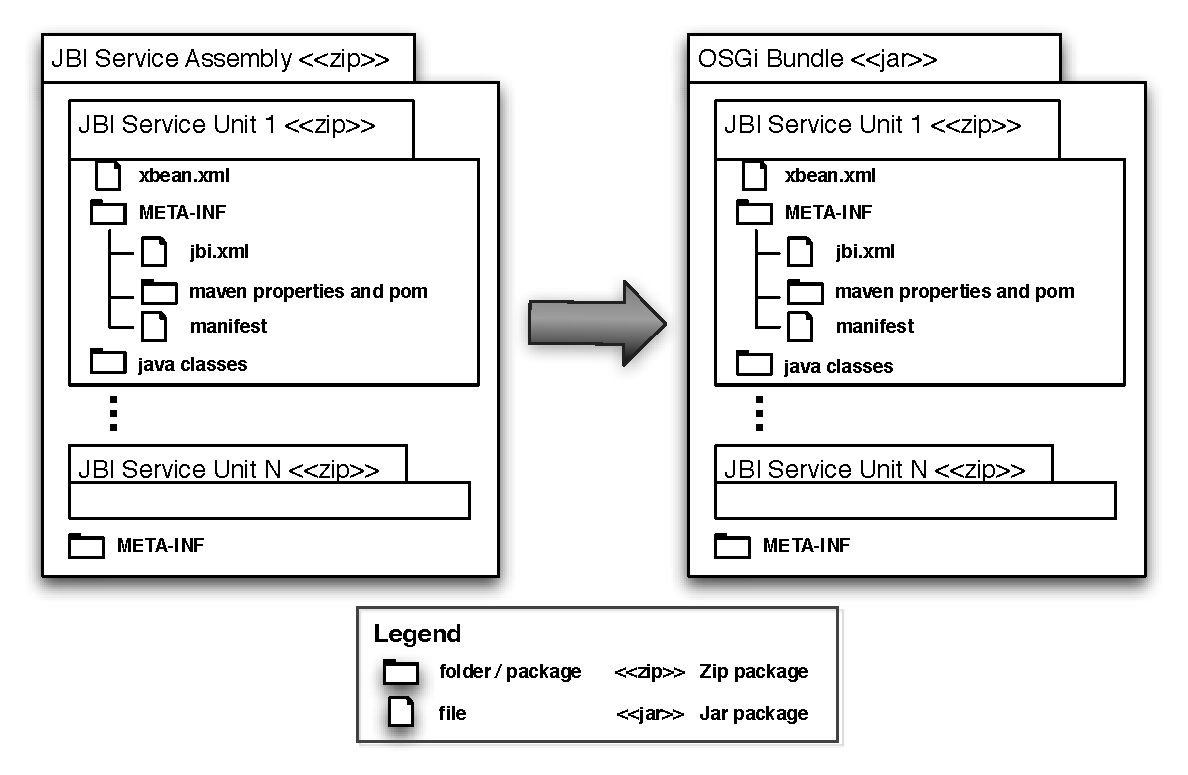
\includegraphics[clip, scale=0.5]{./gfx/osgibundlepackage.pdf}
	\caption[JBI to OSGi repackaging]{ServiceMix 4.x repackaging mechanism for deploying \ac{JBI} components in \ac{OSGi} container.}
	\label{fig:jbitoosgipackage}
\end{figure}

The resources sharing integration level refers to the deployment of \ac{JBI} components in the \ac{OSGi} container, and the utilization of packages exposed by \ac{OSGi} bundles in the \ac{OSGi} container in a loosely coupled manner. The former is part of the integration between containers provided in ServiceMix 4.x versions and described in Figure \ref{fig:jbitoosgipackage}. The deployment mechanism of a \ac{JBI} \ac{SA} into an \ac{OSGi} container is simple: repackaging of the \ac{SA} as a JAR. However, this cannot be consider a full integration in the \ac{OSGi} container. \ac{OSGi} bundles contain in their \term{META-INF} folder one fundamental file for the \ac{OSGi} kernel: the \term{manifest} file. This contains a description of the bundle, the packages it imports, and exports. Imported packages can be either statically stored in the bundle or imported from third party bundles, and exported packages are the ones which exposed to third party bundles. These can be imported with an internal class loading mechanisms developed in the \ac{OSGi} container. The repackaging of the \ac{SA} into a JAR, as it is shown in Figure \ref{fig:jbitoosgipackage}, contains the \term{META-INF} folder, and the \term{manifest} file. However, the latter only contains information about the author, date of creation, but it does not contain information related to the exported packages, and the needed packages to be imported. This \term{manifest} file describes the \ac{SA}, and not the \ac{SU}s. Java classes and package importing description are contained in the \ac{SU} package, and not in the \ac{SA} package. Therefore, the \ac{OSGi} container cannot register in its registry the packages it exports as a service, and cannot load the imported packages to the bundle context. This fact forces us to statically include in the \ac{SA}, and the \ac{SU} the packages which are referenced in each \ac{SU}, and leads to scalability constraints with the tenant-aware deployment process of the system.

ServiceMix 4.x versions are shipped with different \ac{JBI} \ac{BC}s packed as an \ac{OSGi} bundle. However, they are deployed as \ac{OSGi} bundles, and not as \ac{SA}s, in order to enable loose coupling and package sharing between components in the \ac{OSGi} container. ServiceMix-mt allows the deployment of the \ac{JBI} \ac{BC}s, but deployment of \ac{JBI} \ac{BC}s as OSGi bundles is not supported in the JBIMulti2 application. This lack of support forces us to design a second architectural approach, as described in the following sections.

\FloatBarrier

\subsection{Approach 1}

\ac{SQL} database systems provide access to their databases through an endpoint, which is represented as an URL. The native driver used in the data access layer of an application connects to the endpoint, authenticates, sends the query, and reads the response. Therefore, we must support in our system the same operational steps. As discussed in this diploma thesis, the communication protocol varies between different vendors. In this diploma thesis we provide support for incoming MySQL messages. Tenants must access our system through a single physical endpoint. This endpoint is provided by a MySQL proxy which is enriched with authentication, cashing, marshaling, and demarshaling operations. As shown in Figure \ref{fig:designsqlapp1}, the MySQL Proxy Bundle implements the MySQL server operations which are related with the client/server communication protocol. In Figure \ref{fig:designsqlapp1} we specify a server running on port 3306. However, this value can be configured before the deployment of the \ac{OSGi} component. This component is built as an \ac{OSGi} bundle and its packages are exported as services in the \ac{OSGi} container. It interacts with three different components in the system: the \ac{NMR} \ac{API}, the Cache, and the Service Registry. 

Cashing mechanisms are implemented in both the Registry-Cache, and the MySQL Proxy Bundle. The former provides an \ac{API} for creating cache instances, and for persisting and retrieving data. We create a separate cache instance for the \ac{SQL} support due to the need of a custom key creation mechanism which may not coexist in a shared cache between different bundles, as well as the needed isolation of sensible tenant configuration information from third party bundles. The system provides a set of operations which ease the creation of multi-tenant aware keys for persisting frontend authentication data, and queries results form the backend database systems. 

The \ac{NMR} \ac{API} is shipped in ServiceMix as an \ac{OSGi} bundle which exports its \ac{API} as an \ac{OSGi} service. The set of operations included in its \ac{API} allows \ac{OSGi} bundles to create, send, and receive message exchanges to \ac{JBI} endpoints (see Figure \ref{fig:designsqlapp1}).  Before creating the message exchange, the MySQL Proxy Bundle must build dynamically the target endpoint's URL by injecting the tenant context information, and service and endpoint name.

\begin{figure}[htb]
	\centering
		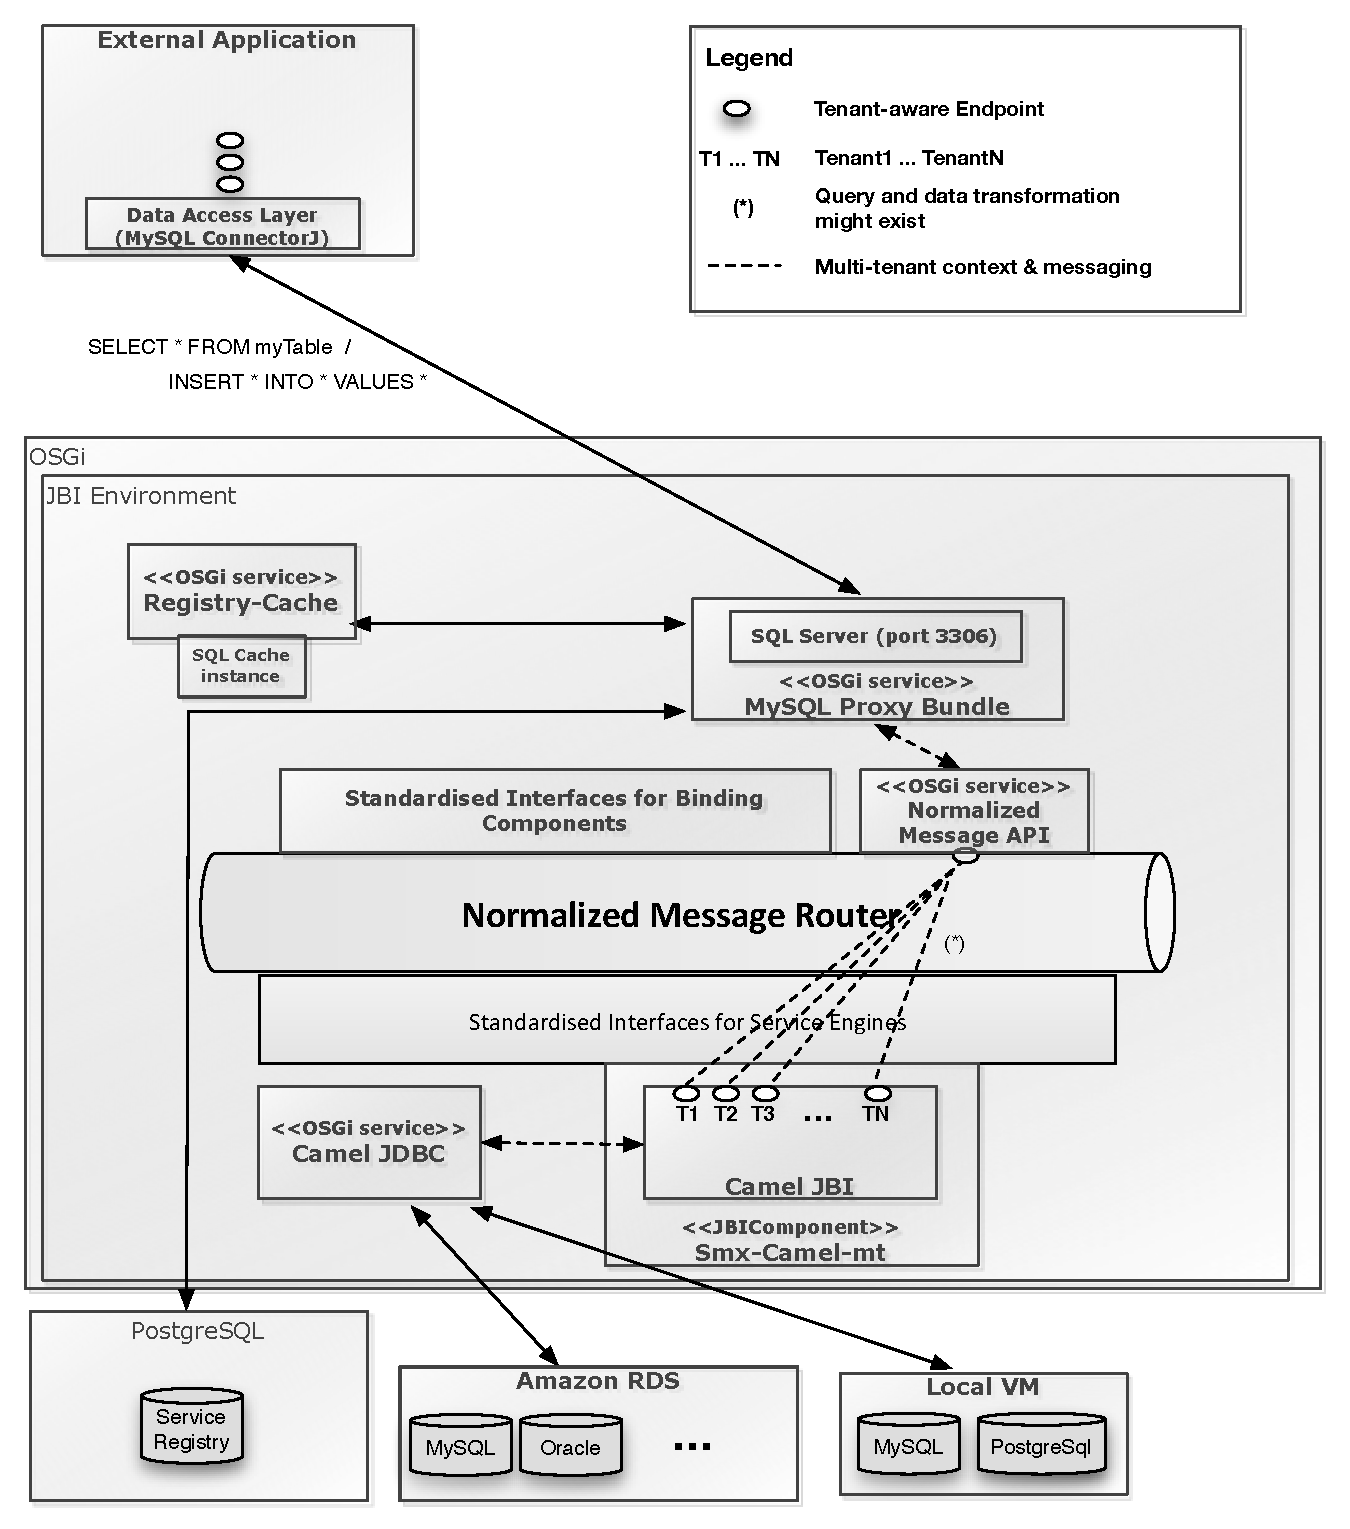
\includegraphics[clip, scale=0.6]{./gfx/sqlApproach/sqlApproachv2_doc.pdf}
	\caption[SQL Support Approach 1]{Architectural overview of the design approach one to support the MySQL communication protocol and routing to backend \ac{SQL} databases.}
	\label{fig:designsqlapp1}
\end{figure}

Apache Camel provides a set of components which integrate most of the communication technologies available in the market. Moreover, it provides an archetype for creating custom components we use in this diploma thesis. ServiceMix provides a Camel \ac{JBI} \ac{BC} which integrates the \ac{JBI} container with the camel router. Muhler extends this component in ServiceMix-mt and enriches it with multi-tenancy awareness. However, the supported multi-tenancy is at the level of tenants, and not at the level of tenant's users. We extend this component and provide user and tenant isolation between endpoints, by injecting the tenant and user UUID in the endpoint's URI (see Listing \ref{lst:endpointuri}). 

%%%%%%%%%%%%%%%%%%%%%%%%%%%%%
\lstinputlisting[float=htb,label={lst:endpointuri},caption={[Tenant-aware Endpoint Configuration]Extended Tenant-aware endpoint URI in extended Backus-Naur Form (EBNF) \cite{Muhler2012}.},style=ebnf]{./gfx/endpointconfiguration.txt}
%%%%%%%%%%%%%%%%%%%%%%%%%%%%%

With multi-tenancy at the tenant and user level, each user can deploy one \ac{JBI} tenant-aware endpoint in the ServiceMix-Camel-mt \ac{SE}. The routes deployed from each tenant-aware endpoint are performed under a different context, and an instance of the targeted component in the route is created. Therefore, with this approach we provide multi-tenancy at the messaging, endpoint, and routing and component context levels. 

Due to the lack of \ac{JDBC} support in ServiceMix for creating provider endpoints, we develop a custom camel component, and enrich it with \ac{JDBC} support for three database systems: MySQL, Oracle, and PostgreSQL. This component is extensible to more database systems when including its native driver, and is build as an \ac{OSGi} bundle and its packages are exported as an \ac{OSGi} service. Messages received from the \ac{NMR} are demarshaled to the backend database system communication protocol, and the response marshaled, correlated, and sent back to the MySQL Proxy Bundle. The demarshalers in this bundle provide the necessary support for transforming the \ac{NMF} response to a MySQL message.

As described in the previous section, ServiceMix-mt provides \ac{JBI} and \ac{OSGi} support and integration, but with some constraints. \ac{JBI} components cannot import packages from \ac{OSGi} bundles exporting its packages. The Servicemix-Camel-mt \ac{SE} provides integration with the camel router for a set of camel components. The camel manual specifies the need for adding statically the custom component packages in the \ac{JBI} \ac{SU} which contains the route definition. Therefore, this leads us to scalability problems in each of the \ac{SA} deployed by the tenants. The \ac{SA} size increases with the new supported database systems, and forces to redeploy all the \ac{SU}s containing the custom camel component when it is modified. This leads to management, storage capacity, and network capacity inconveniences. Hence, we provide a second, and final approach which is very similar to this one, but utilizing the ServiceMix-camel component deployed as \ac{OSGi} bundle. 

\FloatBarrier

\subsection{Approach 2}

In this second architectural design approach we address the scalability problems caused by the \ac{JBI} package dependencies in the \ac{SU}s described in the previous section. This approach is similar to the first one presented, and its main difference relies on the routing from the tenant-aware \ac{JBI} endpoints to the custom camel component \term{cdasmixjdbc} (see Figures \ref{fig:designsqlapp2} and \ref{fig:designsqlapp1}). The functionalities and operations in the MySQL proxy bundle do not differ with the previous approach.
 
\begin{figure}[htb]
	\centering
		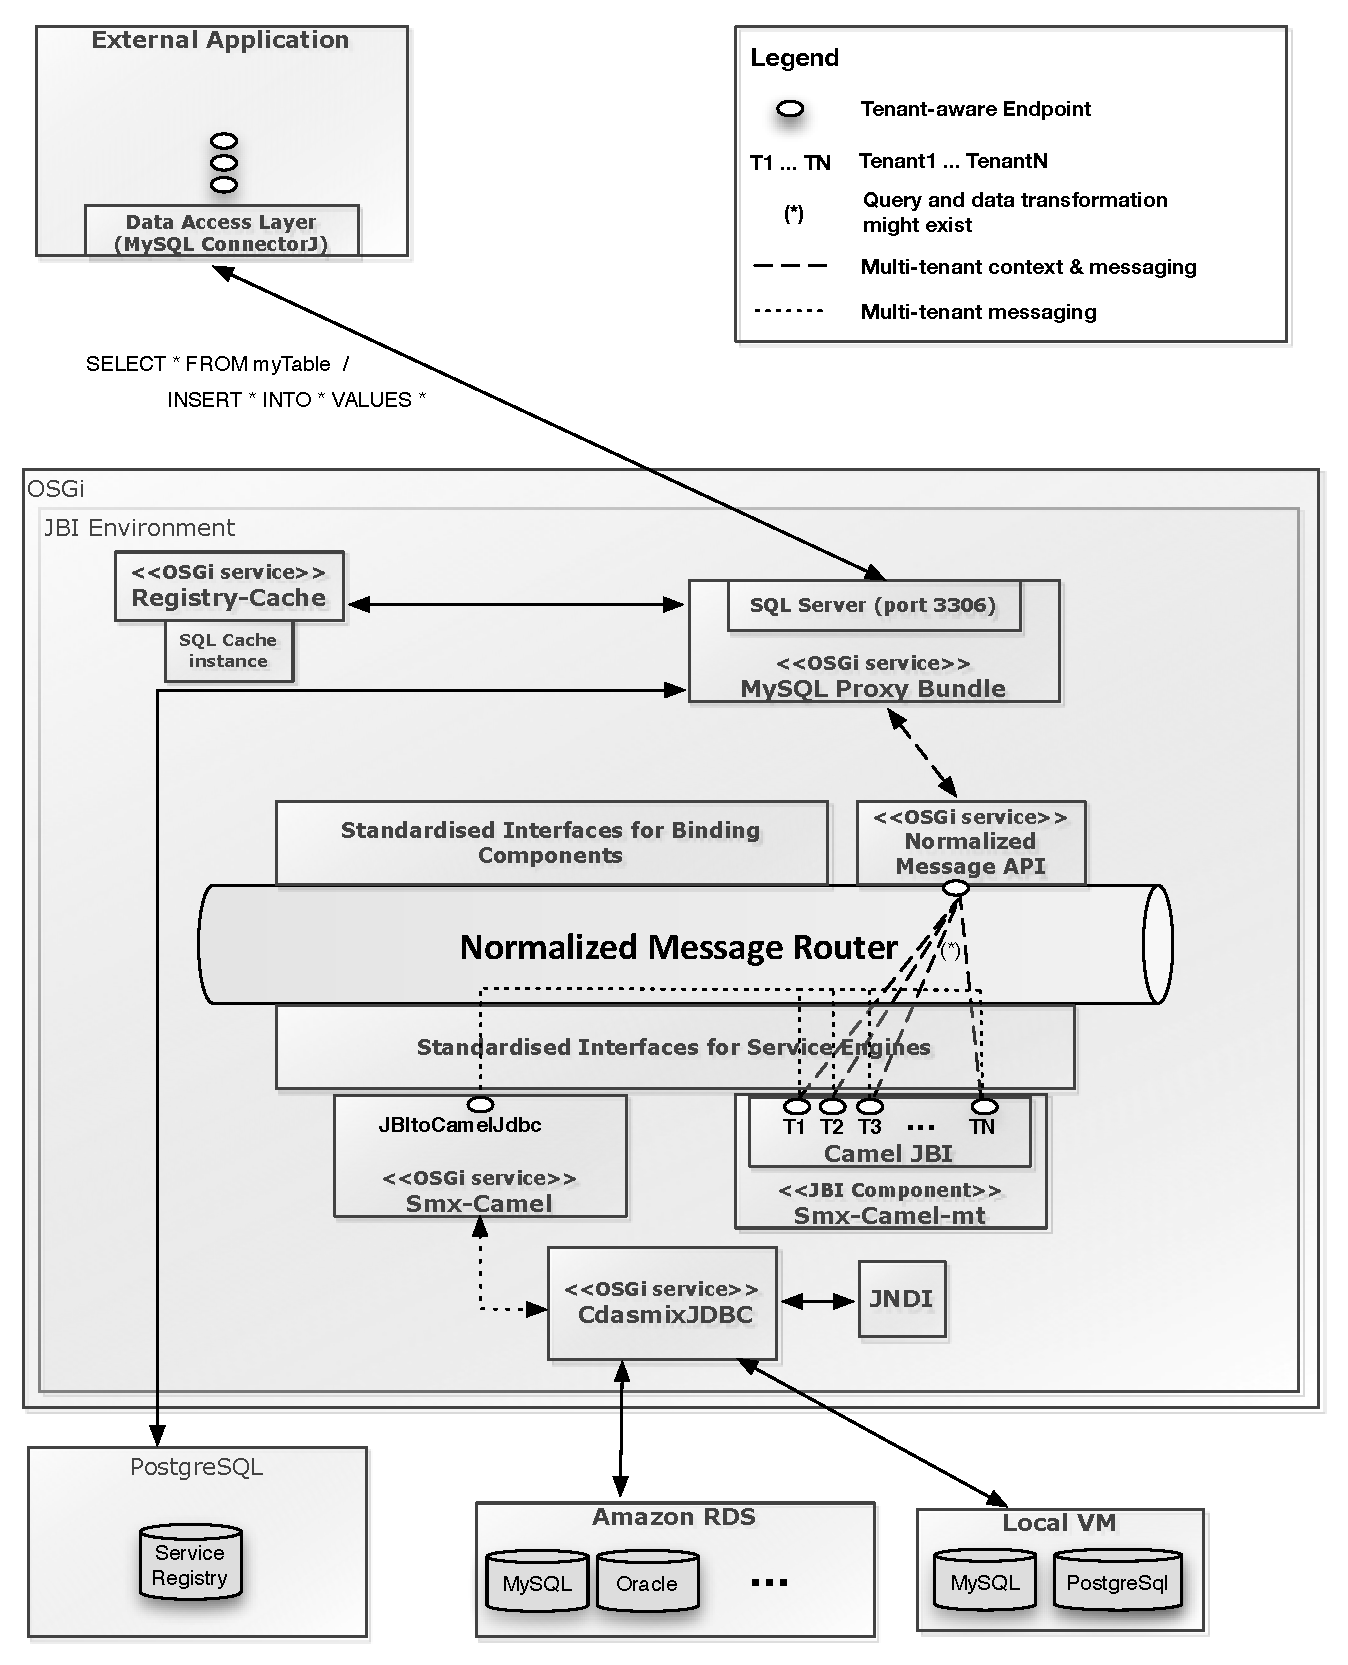
\includegraphics[clip, scale=0.6]{./gfx/sqlApproach/sqlApproachv3_doc.pdf}
	\caption[SQL Support Approach 2]{Architectural overview of the design approach two to support the MySQL communication protocol and routing to backend \ac{SQL} databases.}
	\label{fig:designsqlapp2}
\end{figure}

The message is routed from the MySQL proxy bundle to the tenant-aware \ac{JBI} endpoint deployed in ServiceMix-camel-mt. The multi-tenant message processor instance in ServiceMix-camel-mt routes the message to the \term{JBItoCamelJdbc} endpoint. 

As discussed before, the \ac{JBI} \ac{BC}s deployed in ServiceMix are \ac{OSGi} friendly. This means that the \ac{OSGi} contains a valid manifest file where the description of the bundle, import packages, and export packages are specified. \ac{SU}s deployed on this component are able to reference other \ac{OSGi} packages exposed as a service in the \ac{OSGi} service registry. We provide a single endpoint deployed in the ServiceMix-Camel component where the requests are sent to: the \term{JBItoCamelJdbc} endpoint. When the \term{JBItoCamelJdbc} endpoint is deployed on the ServiceMix-Camel \ac{OSGi} bundle, this searchs in the \ac{OSGi} container for the \term{CdasmixJDBC} component, and creates an instance of the component. Messages routed to the \term{JBItoCamelJdbc} endpoint are then forwarded to the \term{CdasmixJDBC} component, which selects the appropriate \ac{JDBC} native driver, creates a connection, demarshals the request, and forwards the request to the backend Cloud data store server. The connection is established after creating an instance of a \term{DataSource}, which is saved in the \ac{JNDI} registry for future connections, in order to avoid the creation of more than one \term{DataSource} instance per user per backend Cloud data store.

Responses retrieved from the backend Cloud data store are correlated with the initial request and routed back to the MySQL proxy bundle, which demarshals the retrieved data and sends it as a binary \ac{TCP} stream.

In this approach a new instance of the \term{cdasmixjdbc} is not created per tenant endpoint, but is shared between the tenants. Therefore, we cannot ensure an independent component context at the provider endpoint. However, messages contain the tenant information, and the \term{cdasmixjdbc} component interacts with the backend database system establishing separate \ac{JDBC} connections per request. Full multi-tenancy, at the levels of component creation, and endpoint level is not ensured, but it is ensured at the messaging, and context levels. Although full multi-tenancy is not supported, we avoid the deployment of \ac{SU}s which contain the \term{CdasmixJDBC} component in it, and whose size increase may lead to scalability problems in the system. Furthermore, we prevent the deployment of the same component n times, for the n multi-tenant aware endpoints, and prevent future management problems when modifying or upgrading the \term{CdasmixJDBC} component. 

\FloatBarrier



\section{NoSQL Databases}
\label{sec:fundamentalsnosqldb}  

\ac{RDBMS}s ensure data persistency over time and provide a wide set of features. However, the functionalities supported require a complexity, which is sometimes not needed for some applications, and harms important requirements in Web applications or in \ac{SOA} based applications, e.g. throughput. \ac{NoSQL} data stores aim to improve the efficiency of large amount of data storage while reducing its management cost \cite{nosqlcomputerworld}. NoSQL databases are designed to support horizontal scalability without relying on the highly available hardware \cite{strauchnosql}. In a Cloud storage environment where the user sees the available computing and storage resources as unlimited, a \ac{NoSQL} support in a Cloud storage environment might be adequate.

\ac{NoSQL} \ac{DBS} operate as a schema-less storage system, allowing the user to access, modify or freely insert his data without having to make first changes in the data structure \cite{nosql2012}. Cloud providers provide the users with an \ac{API} for accessing, modifying, and inserting data into his isolated container. For example, a user's Amazon Dynamo DB table and item can be accessed by its RESTful \ac{API}, or by installing at the user's side application the Amazon Web Services SDK \cite{amazondynamodb}. Furthermore, it provides the users through its Web-based management console the available management operations. 

Due to the growth of the \ac{NoSQL} support along different Cloud vendors, in this diploma thesis we provide a multi-tenant and transparent communication support for \ac{NoSQL} backend data stores in different Cloud providers. In the following sections we introduce the categorization of the different \ac{NoSQL} databases we aim to support in this diploma thesis, mentioning and giving examples of Cloud data stores available nowadays in the market.

\subsection{Key-value Databases}

In a key-value datastore elements are uniquely identified by an id, which the data store does not take into account its type, and are simply stored as a \ac{BLOB} . A user can get the value for the key, put a value for the key, or delete a key from the data store \cite{nosql2012}. Its storage model can be compared to a map/dictionary \cite{strauchnosql}. Products offering this data storage model in a Cloud infrastructure are Amazon DynamoDB \cite{amazondynamodb}, Google Cloud Storage \cite{googlecloudstorage}, Amazon SimpleDB  \cite{amazonsimpledb} , Amazon S3 \cite{amazons3}, etc. In this diploma thesis we mainly focus on the following key-value data stores: DynamoDB, and Google Cloud Storage.

Amazon DynamoDB's data model includes the following concepts: tables, items, and attributes \cite{amazondynamodb}. The attributes are a key-value, where the value is binary data. Attributes are stored in items, and these are stored in tables. Items stored in a table can be retrieved by referencing its unique id. The number of attributes is not limited by Amazon, but each item must have a maximum size of 64 KB. Accessing stored data in this data store can be mainly done in two ways: using the functionalities provided by the AWS SDK, or using the Cloud storage RESTful \ac{API}. 

Google Cloud Storage's data model includes the following concepts: buckets and objects \cite{googlecloudstorage}. Buckets contain on or more objects. The objects are identified within a bucket with its unique id. Users can perform I/O operations on both buckets and objects. For this purpose, Google Cloud storage provides RESTful \ac{API}.

In this diploma thesis we use an \ac{ESB} for accessing transparently tenant's databases migrated to the Cloud. Servicemix-mt provides multi-tenant \ac{HTTP} support \cite{gomez2012}. Therefore, we reuse and extend the multi-tenant \ac{HTTP} \ac{BC} in order to provide dynamic routing between the different data stores.

\subsection{Document Databases}

Document databases can be considered as a next step in improving the key-value storage model. In this storage model, documents are stored in the value part of the key-value store, making the value content examinable \cite{nosql2012}. Documents with different schemas are supported in the same collection, and can be referenced by the collection's key or by the document's attributes. One of the main difference in the attributes specification regarding \ac{RDBMS} is that in document stores document's attributes cannot be null. When there is an attribute without value, the attribute does not exist in the document's schema. Products implementing this data storage model are Apache CouchDB, MongoDB, etc. \cite{couchdb} \cite{mongodb}.

Mongo DB defines two storage structures: collections and documents \cite{mongodb}. A specific database contains one or more collections identified by its unique id. A specific collection stores one or more documents. Collections and documents stored in a database can be accessed, inserted and modified using the RESTful \ac{API} supported by the database system.

Apache CouchDB defines two storage structures: databases and documents. Data stored in CouchDB are \ac{JSON} documents. The main difference between this two described databases is that MongoDB implements a two step access to the documents: database, collection, and document. Apache CouchDB provides a RESTful \ac{API} for I/O operations.

This databases are not offered by Cloud providers like Amazon or Google, but as a software which can be deployed in user instances, e.g. Amazon EC2 AMI \cite{amazonec2}. 

\subsection{Column-family Stores}

One of the most known Column-family data stores is Cassandra. Column-family data stores store data in column families (groups of related columns which are often accessed together) as rows that have many columns associated with a row key \cite{nosql2012}. This approach allows to store and process data by column instead of by row, providing a higher performance when accessing large amount of data, e.g. allowing the application to access common accessed information in less time.

Cassandra has as its smallest unit of storage the column, which consists of a timestamp and a name-value pair where the name acts as a key \cite{nosql2012}. As in the relational model, a set of columns form up a row, which is identified by a key. A column family is a collection of similar rows. The main difference with the relational model is that each of the rows must not have the same columns, allowing the designer and the application consuming large amounts of data to customize the columns in each row, and the rows in each column family.

Cassandra is not shipped with a RESTful API for I/O operations. However, there are several open-source services layers for Cassandra, e.g. Virgil \cite{virgil}.

\FloatBarrier

\section{Extensions}
\label{sec:extensions}

Apart from the components which we implement in this diploma thesis, we extend existing components developed in the works from Muhler \cite{Muhler2012}, and Uralov \cite{Uralov2012}. We extend the JBIMulti2 application developed by Muhler, and adapt the \ac{JBI} ServiceMix Registry performed by Uralov. 


\subsection{JBIMulti2} 

The multi-tenant aware administration and management application JBIMulti2 offers a list of operations through its Web service interface in order to allow tenants to deploy multi-tenant aware endpoints in ServiceMix-mt. However, it does not provide support for persisting the tenant's Cloud data stores communication meta-data. In Chapter \ref{chap:design} we describe the necessary modifications on the service registry, and the need of extending the application's Web service interface to avoid a connection from the \term{Cloud Data Migration Application} to the database system which stores the tenant configuration data. 

The Service Registry database schema is created using the Java Persistence \ac{API}, and annotating the Java classes with meta-data. We extend the Java class \term{ServiceAssembly}, which stores the \ac{SA}s deployed by the tenant. The \term{ServiceAssembly} class contains the schema representation, and the data storage and retrieval operations.

The Web service interface developed by Muhler \cite{Muhler2012}, and extended by Uralov \cite{Uralov2012}, contains several management operations, e.g. deploy service assembly, create tenant, create user, deploy \ac{JBI} BC, etc., which allows the system administrator and tenants to perform management operations on ServiceMix-mt. The \term{Cloud Data Migration Application} described in Chapter \ref{chap:fundamentals} retrieves from the user the backend database system meta-data, such as access credentials, database name, etc. The application may be hosted on a separate server as JBIMulti2. In order to avoid a direct connection from the \term{Cloud Data Migration Application} to the Service Registry, which contains sensible data, we extend the JBIMulti2 Web service interface, and provide the operations for registering the tenant's backend Cloud data store meta-data. 

\subsection{Cache}

The cashing support in ServiceMix-mt is provided in the \ac{OSGi} component \ac{JBI} ServiceMix Registry. Uralov provides a set of operations to set up a cache instance, store elements, and retrieve stored elements \cite{Uralov2012}. However, the \ac{JBI} ServiceMix Registry \ac{OSGi} bundle libraries are not registered as an \ac{OSGi} service. Therefore, this component is not accessible from third party \ac{OSGi} bundles in the \ac{OSGi} container. We modify its original \term{BundleActivator} class and include the \ac{OSGi} service registration to allow its usage from external \ac{OSGi} bundles.

\lstinputlisting[label={lst:ehcacheconfig},caption={[EhCache Configuration for SQL Support]Eh cache configuration for \ac{SQL} support.},style=xml]{./gfx/ehcacheconfig.xml}

The cache instances are created on the Ehcache 2.6.0 component \cite{ehcache}, which provides support to store serializable objects indexed by a key. A cache instance configuration in the Ehcache component must be specified in an \ac{XML} file, which is described in Listing \ref{lst:ehcacheconfig}. However, the cashing support is not multi-tenant aware. We implement a dynamic creation of multi-tenant aware cache keys in order to ensure isolation between the cashed tenant's information, and data (see Listing \ref{lst:cachekey}). 

\FloatBarrier

\chapter{Validation and Evaluation}
\label{chap:validationevaluation}

%In order to ensure that  we fulfill the requirements listed in Chapter \ref{chap:spec}, in this chapter we provide a testing of the main components we implemented and we describe how we initialize the different testing scenarios. In Section \ref{sec:multitenanttest} we provide three different testing scenarios, one per extended \ac{BC}, and we monitor both incoming and outgoing messages to and from the \ac{ESB}.

In this chapter we provide the validation, and evaluation of the system. We must ensure that the requirements specified in Chapter \ref{chap:spec} are fulfilled in the design and implementation phases. In Section \ref{sec:deploymentandinit} we describe the steps which should be followed to initialize the system, and the testing scenarios. After the initialization we execute the test cases in Section \ref{sec:validation}, and monitor the incoming requests to ServiceMix-mt, and the outgoing requests to the backend Cloud data store. Due to the extensions implemented on the \ac{ESB}, we evaluate in Section \ref{sec:evaluation} its behavior, and the impact that our modifications have on the original ServiceMix-mt.

\section{Deployment and Initialization}
\label{sec:deploymentandinit}

The validation and evaluation of the prototype must close to the motivating scenario. Therefore, we must perform the testing of the prototype in a Cloud environment. We are provided with a VM image in the FlexiScale Cloud infrastructure \cite{flexiscale}, which runs the operative system Ubuntu 10.04 64 bits. The following components are deployed in the VM:
\begin{itemize}
	\item ServiceMix-mt 4.3.0: the multi-tenant aware ServiceMix 4.3.0. In addition to the \ac{OSGi} bundles, \ac{JBI} \ac{SA}s, and JBIMulti2 shared library \cite{JBIMulti2Man}, in its deploy folder we store the \ac{JBI} ServiceMix Registry, CDASMix MySQL Proxy, and the CamelJDBCCdasmix \ac{OSGi} bundles for deployment. 
	\item JOnAS 5.2.2: the Java application server which hosts the JBIMulti2 application. 
	\item MySQL database 5.1: MySQL database system for performing evaluation and validation of the prototype with a local database instance.
	\item PostgreSQL 9.1.1:  PostgreSQL database system which stores the tenant-aware configuration data in the Service Registry, Configuration Registry, and Tenant Registry. 
\end{itemize} 

For more information about the deployment, and initialization of the ServiceMix-mt and JBIMulti2 please refer to the document "Manual for the JBIMulti2 Implementation" \cite{JBIMulti2Man}. On the other hand, we utilize de following off-premise instances:
\begin{itemize}
	\item Amazon RDS db.m1.micro instance: MySQL 5.5 database system hosted in the Amazon RDS Cloud infrastructure. 
	\item Amazon DynamoDB table: \ac{NoSQL} key-value database for storing objects in the created tables. 
	\item Google Cloud Storage: \ac{NoSQL} key-value database for storing buckets and objects.
\end{itemize} 

We must maximize the approximation of the testing and evaluation scenarios with the motivating scenario. Therefore, we perform the testing cases from a local machine in the University of Stuttgart network infrastructure, in order to simulate the access to the data from an on-premise data access layer. Communication with the JBIMulti2 application for tenant configuration, and deployment of \ac{SA}s is established using soapUI 3.6. Communication with the MySQL endpoint in ServiceMix-mt is established using the MySQL Connector/J 5.1.22, while for the different tenant-aware \ac{HTTP} endpoints we use the Java libraries provided by the Cloud data store providers. 
\section{Validation}
\label{sec:validation}

In this section we provide an overview of the messages, and programs used for the validation of the prototype. The transmission of the following message samples requires the system to be started, and the operations until the deployment of the tenant operator's \ac{SA} to be executed. These messages are provided in a soapUI test suite shipped with the prototype. From the moment when the tenant deploys the \ac{SA}, the configuration of the frontend and backend data stores can be associated to it. The data store configuration is done through the execution of operations which are accessible through a Web service interface. Therefore, either the \term{Cloud Data Migration Tool}, or the tenant can configure their database connections through the \ac{ESB} to the backend Cloud data store where his data is migrated to.
 
\lstinputlisting[label={lst:testaddds},caption={[Add Source and Target Data Source Sample Request]Add Source and Target \ac{SQL} Data Source \ac{SOAP} over \ac{HTTP} sample request.},style=xml]{./gfx/addds.xml}

The message described in Listing \ref{lst:testaddds} contains the needed information for registering and providing access to the tenant operator A in the MySQL CDASMix Proxy, and connecting with an \ac{SQL} database system in a backend Cloud data store. The tenant operator must authenticate with JBIMulti2 in order to register the connection meta-data, e.g. protocol, URL, database type, access credentials, etc. In Listing \ref{lst:testaddds} the tenant operator A, which is a user of the tenant Taxi Company, registers for the endpoint configuration described in the \term{servicemix.cdasmix.jbi.camelSA} a connection with a MySQL 5.1.3 database system instance in the Amazon RDS infrastructure. When more than one target database system wants to be attached to an existing source data source registered in the system, this provides the \term{AttachTargetDataSource} operation, which has as pre-condition the existence of the specified source data source.

\lstinputlisting[label={lst:testaddmis},caption={[Add Source and Target Main Information Structure Sample Request]Add Source and Target  \ac{SQL} Main Information Structure \ac{SOAP} over \ac{HTTP} sample request.},style=xml]{./gfx/addmaininfosql.xml}

When the source and target data source configuration are registered, the tenant operator (or through the \term{Cloud Data Migration Tool}) can register the storage structure meta-data of his database. For example, for a MySQL database system instance in Amazon RDS, the tenant operator must provide the tables' name (see Listing \ref{lst:testaddmis}), or for a bucket stored in a backend Google Cloud Storage container the tenant must provide the bucket identifier.

\lstinputlisting[label={lst:testaddsis},caption={[Add Source and Target Secondary Information Structure Sample Request]Add Source and Target \ac{NoSQL} Secondary Information Structure \ac{SOAP} over \ac{HTTP} sample request.},style=xml]{./gfx/addsecinfonosql.xml}

Registration of secondary information structure meta-data applies only for \ac{NoSQL} databases. The message described in Listing \ref{lst:testaddsis} contains the registration meta-data for an item stored in a table in the Amazon DynamoDB infrastructure. 

After the migrated data's meta-data is registered in the system, the tenant operator can access transparently the system using the standardized database access protocols, e.g. MySQL for the MySQL database system, and \ac{HTTP} for \ac{NoSQL} databases. 

\lstinputlisting[label={lst:testjdbc},caption={[Test Retrieving Information from Backend and Local Data Store]Retrieve data via \ac{JDBC} and MySQL protocol migrated to a backend Cloud data store, or local database system.},style=xml]{./gfx/testclient.java}

In Listing \ref{lst:testjdbc} we provide part of a Java program which connects via the MySQL Connector/J native driver with the MySQL CDASMix Proxy component on the port 3311. The options attached to the connection URL must be set as in the provided code in order to increase the performance of the communication, e.g. multi-querying for multiple queries in one statement, cache server configuration in order not to request the server configuration data per request, etc. In the MySQL request in Listing \ref{lst:testjdbc}, the tenant operator authenticates with the tenant and user UUID, and its password. Password is read in the system, but it is not compared in the authentication process, as the CDASMix MySQL proxy does not implement the hashing mechanisms of a MySQL server. After successful authentication, it executes a query which contains multiple queries in the same request. Each query is processed independently in the system when retrieving information from the different backend database systems, e.g. the \term{customer} table is stored in Amazon RDS, while mainInfoTest4 and mainInfoTest1 are stored in the local MySQL database system. The response is received as a single statement which contains n result sets, one for each query in the multi-query. 

\FloatBarrier
\chapter{Performance Evaluation}
\label{chap:performanceevaluation}

In the following sections we provide the requirements which should fulfill the performance evaluation of the \ac{ESB} solution we extend for multi-tenancy awareness. For this purpose, we extend a load generator developed by AndroitLogic to enable it with tenant-aware messaging \cite{androit2012}. Finally, we provide an overview of the components and systems involved in the different scenarios of the evaluation, and the design approach and implementation of the extension.

\section{Specification}
\label{sec:evaluationspecification}



\subsection{Evaluation Requirements}
\label{sec:evalrequirements}

% different message size, reduce loose couple being able to specify different types of messages
% invoke the endpoints with concurrent users and invoke endpoints concurrently
% be able to set the number of concurrent users and concurrent endpoints to invoke at the same time
% include multi-tenancy awareness in the benchmark for the different scenarios
% structured data as the output for analysis, for throughput and response time for the different messages requests for the different endpoints
% has to be done on top of the androitbenchmark, so that we can reuse and extend their benchmark
% system measurements of cpu and memory in structured data. also the measurement of the heap size (real memory consumtion) in the process
% monitoring of number of outgoing requests and incoming requests into the backend service, wireshark

In this student thesis we provide a performance analysis on the integration of the multi-tenant aware approaches in ServiceMix and measure the impact on the performance of the extended prototype. For this purpose, we need to fix which measurements we use for the evaluation. The driver should perform the following measurements: response time (measured in milliseconds) and throughput (measured in number of messages sent per second) respect to a backend service, and CPU and memory usage of the system hosting the instance of ServiceMix. The evaluation has to be done in different scenarios, each of them sending different messages number and sizes, for different multi-tenant and non multi-tenant aware endpoint configurations, as described in Table \ref{tab:evaluation} \cite{EvalESB}.

\begin{table}[htbp]
\centering
\begin{tabular}{llll}

	\toprule
	 Number of Endpoints 		& Messages Size	& ServiceMix Instances		& Multi-tenancy awareness 		\\
	 \midrule
	 
	 1 						& 0.5 / 1 KB 		& 1						& mt and non-mt									\\
	  						& 				& 2						& non-mt											\\
	 2 						& 0.5 / 1 KB 		& 1						& mt and non-mt									\\
	  						& 				& 2						& non-mt											\\
	 4 						& 0.5 / 1 KB 		& 1						& mt and non-mt									\\
	  						& 				& 2						& non-mt											\\
	 10 						& 0.5 / 1 KB 		& 1						& mt and non-mt									\\
	  						& 				& 2						& non-mt											\\														
	 
	\bottomrule
\end{tabular}
\caption[ServiceMix evaluation performance scenarios]{Specification of the different scenarios to be evaluated. In both multi-tenant and non multi-tenant aware evaluations, one user per endpoint / tenant is configured. \\ \term{Legend: mt (multi-tenant aware), non-mt (non multi-tenant aware)}}
	\label{tab:evaluation}
\end{table}

AndroitLogic has developed a performance analysis driver which fulfills most of the above requirements in different scenarios \cite{androit2012}. In our evaluation, we extend the Direct Proxy scenario from the AndroitLogic  \ac{ESB} Performance benchmark \cite{androit2012}. However, it doesn't achieve one of the main requirements of this student thesis: multi-tenant aware messaging and concurrent invocation between endpoints. Those two requirements should be included in an extended version of the primitive driver. Furthermore, the extension should be utilized with different \ac{ESB} solutions and must be user-friendly configurable for the different scenarios. The output of the driver measurements should be analyzed, therefore the output data must be in structured format. 

\input{evaluation/evaluationoverview}

\FloatBarrier
\section{ESB Performance Evaluation Architecture}
\label{sec:esbevaluationdesign}

% explain the figure
% the evaluation is done for SOAP over HTTP protocols based on a in only message exchange patter, so that we are only masuring how much time does it take to reach the backend service. explain that the dashed lines are because those calls are optional, this means, we divide in to more than one scenario, each scenario testing 1, 2, 4, and 10 endpoints
% for the two instances of servicemix, we provide 10 endpoints in total, and 5in each instance, and the load is divided into the endpoitns. we start with the scenario with 2 endpoints
% explain a little bit the java bench androitlogic driver
% explain that we will use differente messages for the scenarios so that we can decouple them from the scenarios, being able to modify messages independently. results are in a format (I can paste an example of a result from the java benchmark) and then the driver provided by androit to be able to convert it to a csv file
% for concurrent calls between endpoints, we are going to create as many instances of the java benchmark as many endpoints we want to call concurrently by using shell scripting and the & (background task). Explain how many messages we are sending, in factor 2..., and the warmup phase of the esb, so that we ensure that the heap mamory is cleaned (garbage collector)
% system monitoring for the %CPU and %sys memory using the top command and then converting the output data to csv
% jconsole usage for heap measurements
% wireshark just for counting the packages that arrived and pack lost
% to fill the messages, we fill it with random characters and create a <attachment> part in the body

AndroitLogic has developed in their \ac{ESB} Performance Evaluation Round 3 a load generator for different scenarios. After analyzing its main features, we found it suitable for our work, but only if we can include tenant-awareness in the execution. We evaluate the \ac{SOAP} over \ac{HTTP} communication protocol in both native ServiceMix \ac{HTTP} \ac{BC} and in the multi-tenant \ac{HTTP} \ac{BC}. With this we want to evaluate not only the performance of the \ac{ESB} solution we are using in our Cloud infrastructure, but also the penalty caused by the multi-tenant awareness implementation. The \ac{SOAP} over \ac{HTTP} protocol is well known for its usage in Web services. In this evaluation we use as a backend Web service an Echo Service which logs the received requests. For this purpose, we must push the scenarios as close as possible to a real Web service consumption. Therefore, we divide the evaluation system in two virtual machines connected by a network (see Figure \ref{fig:evaluationarchitecture}). 


%%%%%%%%%%%%%%%%%%%%%%%%%%%%%
\begin{figure}[htb]
	\centering
		\includegraphics[width=.95\textwidth, trim=0.0cm 0.0cm 0.0cm 0.0cm, clip]{./gfx/evaluationarchitecture.pdf}
	\caption[ESB Performance Evaluation Architecture]{Architectural overview of the components used for the evaluation of the \ac{ESB} performance. \textbf{Note:} We evaluate only ServiceMix, not the integrated version of ServiceMix with the JBIMulti2 application, in order to be able to perform a direct comparison between the multi-tenant and the non multi-tenant ServiceMix.}
	\label{fig:evaluationarchitecture}
\end{figure}
%%%%%%%%%%%%%%%%%%%%%%%%%%%%%


The virtual machine one hosts the front and backends components: performance benchmark and the Web service. The Web service is deployed in an Apache Tomcat server. The extended performance benchmark is built of the following components: AndroitLogic driver, shell scripts and data converters. The AndroitLogic driver support concurrent users invoking the same endpoint, but not concurrent users between two or more endpoints. Furthermore, it does not support message modification for including tenant information. For this purpose, we have designed the shell scripts which can give support on those two requirements (see Figure \ref{fig:evaluationarchitecture}). In the first place, the shell script modifies or does not modify the message which will be sent by the driver. In the second place, we perform concurrent invocations between endpoints by creating several Unix background tasks of the driver. Each of the tasks results can be dumped in a shared file between the driver instances. However, the results come in non structured format for analysis. Therefore, we convert the data using a converter provided by AndroitLogic \cite{androit2012}. For monitoring the packet lost rate, we will listen on the server's port where the Web service listens with a well known monitoring tool, Wireshark \cite{wireshark}.

We use the virtual machines two and three for hosting the ServiceMix instances. The two instances are used only in non multi-tenant scenarios. For both multi-tenant and non multi-tenant scenarios we must increase the number of concurrent calls to the endpoints. In the requirement we specify scenarios of one, two, four, and ten endpoints. The system performance measurement can be done by system commands. We provide a component which take CPU and Memory measurements and converts its output to structured data for analysis. However, the system memory usage measurements do not give variable percentages over time. The percentage shown is the one associated with the memory consumption of the JVM the \ac{ESB} runs on, which is previously reserved and fixed over time. To get more representative data, we measure the heap consumption of ServiceMix in the JVM using Java Console, which give us a better representation of the variability between the different scenarios (See Figure \ref{fig:evaluationarchitecture}). For monitoring the communication, an instance of Wireshark can also be used, but in our evaluation it is optional.


\FloatBarrier
\clearpage
\section{Evaluation}
\label{sec:evaluation}

In this section we first describe the components we implemented to be able to reuse the existing load performance driver from AndroitLogic \ac{ESB} Performance Round 6 and adapt it to the required multi-tenant scenarios \cite{androit2012}. In Section \ref{sec:evaluationanalysis} we shortly describe the deployment and initialization in the virtual machines under the Flexiscale network \cite{flexiscale} and we evaluate the results obtained from the different scenarios. 

\subsection{ESB Performance Evaluation Benchmark}
% put a figure of the folder skeleton
% explain the androit benchmark (we can put an example of the inputs of the java call)
% explain the endpoint configuration (both multi-tenant and non multi-tenant)
% echo service at the end
% message sample (and explain that we will use the message sample to include the tenant id and user id in the to and from values) so that we can see them in the echo service
% endpoint configuration, for both multi tenant and non multi tenant

AndoitLogic has developed an ESB Performance Benchmark in their Round 6 \cite{androit2012}. Their benchmark evaluates the ServiceMix behavior under different scenarios, which vary in the request message size, number of requests per endpoint, and number of concurrent users per endpoint. Their load generator is included in the \term{org.adroitlogic.toolbox.javabench} package in their Management Toolbox application \cite{androit2012}. They provide an HttpBenchmark and a \term{data to csv format} converter. The former makes \ac{HTTP} POST requests to the specified endpoint URL, and generates performance statistics, e.g. response time, throughput. The latter converts the driver's results to structured data for analysis. We reuse both components, but develop components on top which create several instances of the \term{javabench} to invoke multiple endpoints concurrently. Furthermore, we need to add tenant context information before invoking the driver. The components are implemented in UNIX shell scripts.

%%%%%%%%%%%%%%%%%%%%%%%%%%%%%
\begin{figure}[htb]
	\centering
		\includegraphics[width=.95\textwidth, trim=0.0cm 0.0cm 0.0cm 0.0cm, clip]{./gfx/folderorganizationesbperformance.pdf}
	\caption[ESB Performance Evaluation Package Structure]{Overview of the package used for the evaluation of the \ac{ESB} performance}
	\label{fig:folderarch}
\end{figure}
%%%%%%%%%%%%%%%%%%%%%%%%%%%%%

In Figure \ref{fig:folderarch} we describe the overall structure of our loader package. We define three scenarios: scenario 1 is non multi-tenant aware and with one instance of ServiceMix, scenario 2 is non multi-tenant aware with two instances of ServiceMix, and scenario 3 is multi-tenant aware with 1 instance of ServiceMix \cite{EvalESB}, \cite{EnablingMT}. The \ac{SOAP} messages and the endpoints' URLs are read from \ac{XML} files stored in the \term{scenariox} folder. The messages vary from 500B to 100K. However, in this student thesis we perform the analysis for the 500B and 1K messages' sizes. The main and secondary scripts used in this analysis are located under the main scripts folders and the results generated are stored in the \term{ResultsScenariox} folder. In addition, for the multi-tenant scenarios, the endpoint URL file must also contain the tenant context information, e.g. tenantId and userId. 

For the evaluation scenarios we create using the ServiceMix \ac{HTTP} maven archetype 11 \ac{SU}s. Ten \ac{SU}s contain non multi-tenant endpoint configurations of 10 consumer and 10 providers which support the \ac{SOAP} over \ac{HTTP} communication protocol, while one \ac{SU} is configured to be deployed on the multi-tenant \ac{HTTP} \ac{BC} by 10 tenants, generating 10 tenant-aware endpoints (10 tenant-aware consumer and provider endpoints). The deployment phase is described in Section \ref{sec:evaluationanalysis}.

%%%%%%%%%%%%%%%%%%%%%%%%%%%%%
\lstinputlisting[label={lst:scenarioinvokationi},caption={[ESB Performance Analysis Main Shell Script Invocation] Invocation parameters in the main shell scripts of the benchmark.},basicstyle=\scriptsize]{./gfx/androitinvokation.txt}
%%%%%%%%%%%%%%%%%%%%%%%%%%%%%

For the non multi-tenant scenarios, we specify the needed invocation parameters in Listings \ref{lst:scenarioinvokationi}, \ref{lst:loopinvokation}, and \ref{lst:loopinvokation2}. The non multi-tenant aware shell script takes as one of the input parameters the file path where the \ac{SOAP} message is stored and creates the result scenario file name based on the message size and the running scenario. Furthermore, the endpoints' URLs are retrieved from the endpoint configuration file and the script reads as many URLs as tenants we specify. For supporting concurrent calls between endpoints, we create as many instances of the \term{javabench} as endpoints by running a secondary script, the loop script (see Figure \ref{fig:folderarch}), which is executed as a Linux background task. The scenario is divided in two phases: warm-up and performance test. In the warm-up phase an amount of requests are concurrently sent to the endpoints in order to warm-up the \ac{ESB} and get consistent results, while in the performance test phase we perform the measurements which can be analyzed. In the warmup phase the initial request number is set to 10240 requests. This value is then increased exponentially, and divided by the number of endpoints, as described in the following explanation. The loop script increments exponentially the number of requests and divides it by the number of endpoints in the \ac{ESB}, e.g. during the performance test phase if an initial request number is set to 20, then it sends to each endpoint \begin{math} 20 * 2^i, i = [1,2,3,5,6] \end{math} divided by the number of invoked endpoints in the scenario. The same sequence is applied for the multi-tenant scenario. 

%%%%%%%%%%%%%%%%%%%%%%%%%%%%%
\lstinputlisting[label={lst:loopinvokation},caption={[ESB Performance Analysis Non Multi-tenant Shell Script Invocation]Invocation parameters in the non multi-tenant shell script of the benchmark.},basicstyle=\scriptsize]{./gfx/loopinvokation.txt}
%%%%%%%%%%%%%%%%%%%%%%%%%%%%%

The approaches taken into account for the non multi-tenant scenarios are similar to the multi-tenant scenario, as it is shown in Listing \ref{lst:loopinvokation}. The main difference relies on the need of tenant context information injection before the \ac{SOAP} message is read and sent over \ac{HTTP} concurrently to the tenant-aware endpoints. The concurrent reading of messages leads us to the need of using temporal files to store the messages containing tenant context information. The temporal files are created in the same directory as the requests files, and we modify the content by reading the original request in the loop2 script shown in Listing \ref{lst:loopinvokation2} and using the Linux \term{sed} command to inject the tenant context information read from the endpoints' URL definition file. 

%%%%%%%%%%%%%%%%%%%%%%%%%%%%%
\lstinputlisting[label={lst:loopinvokation2},caption={[ESB Performance Analysis Multi-tenant Shell Script Invocation]Invocation parameters in the multi-tenant shell script of the benchmark.},basicstyle=\scriptsize]{./gfx/loopinvokation2.txt}
%%%%%%%%%%%%%%%%%%%%%%%%%%%%%

With the above approaches we fulfill the requirement of getting the response time and the throughput when invoking and external Web service through an \ac{ESB}. We have also implemented scripts for monitoring the system resources with the \term{top} Linux command and with the Java Console \cite{jconsole}. The former provides data at the system level, e.g. JVM memory consumption, while the latter provides data about the exact amount of JVM resources the ServiceMix process consumes.


\subsection{ESB Performance Evaluation Analysis}
\label{sec:evaluationanalysis}

	In this student thesis we extend and add extra functionality to ServiceMix. Therefore we need to measure its behavior and compare it with the baseline, which is the non multi-tenant version of Apache ServiceMix 4.3.0 \cite{ASM}. In the following sections we describe the systems we use for evaluating the performance of the \ac{ESB}, and we discuss some of the results we obtained. 

	\subsubsection{Deployment and Initialization}
	
	The different scenarios we run in this evaluation must approximate as much as possible to real scenarios. Thus we utilize three Ubuntu 10.04 virtual machines in this evaluation connected by the network in the Flexiscale infrastructure \cite{flexiscale}. One virtual machine hosts the evaluation package and an echo Web service which implements the In-Only \ac{MEP} and is deployed in Tomcat 7.0.23. Wireshark 1.2.7 is installed for monitoring incoming and outgoing requests to and from the echo Web service. In a second and third virtual machine we install one instance of ServiceMix 4.3.0 and the system resources measurement scripts. We have listed in Section \ref{sec:evaluationspecification} a set of multi-tenant and non multi-tenant scenarios. For the non multi-tenant scenarios we have deployed in the ServiceMix \term{deploy} directory a \ac{SA} containing the configuration of 10 consumer and 10 provider endpoints. For the multi-tenant scenarios we performed the operations described in Section \ref{sec:multitenanttest} and deploy through JBIMulti2 10 tenant-aware consumer and 10 tenant-aware provider endpoints. Both tenant-aware and non tenant-aware endpoints must be specified in the endpoint file the extended driver reads for sending the \ac{SOAP} requests.
	
	
	\subsubsection{Evaluation Analysis}
	
	%%%%%%%%%%%%%%%%%%%%%%%%%%%%%
	\begin{figure}[htb]
		\centering
			\includegraphics[clip, scale=0.5]{./gfx/response1K.pdf}
		\caption[ESB Performance Evaluation Response time for 1KB Messages]{Response time of the different scenarios for 1KB \ac{SOAP} over \ac{HTTP} requests \cite{EvalESB}.}
		\label{fig:responsetime}
	\end{figure}
	%%%%%%%%%%%%%%%%%%%%%%%%%%%%%
	
	The numerical values obtained from the communication driver are distributed per endpoint. Therefore, we make the average between the endpoints for each set of sent requests. The latency when increasing the number of endpoints in the system increases between 25\% and 45\% for concurrent requests sent to 2, 4 and 10 endpoints (see Figure \ref{fig:responsetime}). We can see that our extended version declines the original ServiceMix's performance approximately 30\% \cite{EvalESB}. Furthermore, we can observe that the response time for the different multi-tenant scenarios does not increase proportional to the number of tenants, but shows a better performance per endpoint. When distributing the requests between two ServiceMix instances we have observed that the response time is substantially reduced when increasing the number of endpoints.	
	
	%%%%%%%%%%%%%%%%%%%%%%%%%%%%%
	\begin{figure}[htb]
		\centering
			\includegraphics[clip, scale=0.7]{./gfx/evaluation_throughput.pdf}
		\caption[ESB Performance Evaluation Throughput for 1KB Messages]{Throughput of the different scenarios for 1KB \ac{SOAP} over \ac{HTTP} requests \cite{EvalESB}.}
		\label{fig:evaluationthroughput}
	\end{figure}
	%%%%%%%%%%%%%%%%%%%%%%%%%%%%%	
		
	When measuring the throughput, the analysis took us to the same deduction we discussed above. When the number of endpoints decreases, we can observe a bigger gap between the native and the extended version of ServiceMix. As we increase the number of endpoints, e.g. 10 endpoints, we can see that the gap between approaches is exponentially narrowed (see Figure \ref{fig:evaluationthroughput}).  
	
	%%%%%%%%%%%%%%%%%%%%%%%%%%%%%
	\begin{figure}[htb]
		\centering
			\includegraphics[clip, scale=0.5]{./gfx/evaluation_cpu.pdf}
		\caption[ESB Performance Evaluation CPU Consumption]{Overview of the CPU consumption over the different scenarios \cite{EvalESB}.}
		\label{fig:evaluationcpu}
	\end{figure}
	%%%%%%%%%%%%%%%%%%%%%%%%%%%%%
	
	Finally, we have analyzed the CPU consumption of the process running the ServiceMix instance. We can observe in the average CPU consumption that there is a gap between both multi-tenant and non multi-tenant scenarios which increases when the number of endpoints increases. However, when increasing the number of endpoints the average CPU consumption stabilizes and maintains close to a constant value. The maximum CPU consumption values decreases in the non multi-tenant scenarios when increasing the number of endpoints, while for the multi-tenant scenario it linearly increases from two endpoints. In the 4 or 10 endpoints scenarios, the maximum CPU consumption difference between the native and the extended approaches are between 250\% and 320\% approximately (see Figure \ref{fig:evaluationcpu}).

The tenant authentication procedure demands a greater number of resources when parsing the \ac{SOAP} headers and the \ac{XML} data from the tenant context file. However, this decline caused by the implemented authentication procedure and the marshaling of tenant context information within the process is much lower that the decline caused by establishing a connection with an external database system and retrieving the tenant context information from an external source to the process.  
	
	




%\chapter{Performance Evaluation}
\label{chap:performanceevaluation}

In the following sections we provide the requirements which should fulfill the performance evaluation of the \ac{ESB} solution we extend for multi-tenancy awareness. For this purpose, we extend a load generator developed by AndroitLogic to enable it with tenant-aware messaging \cite{androit2012}. Finally, we provide an overview of the components and systems involved in the different scenarios of the evaluation, and the design approach and implementation of the extension.

\section{Specification}
\label{sec:evaluationspecification}



\subsection{Evaluation Requirements}
\label{sec:evalrequirements}

% different message size, reduce loose couple being able to specify different types of messages
% invoke the endpoints with concurrent users and invoke endpoints concurrently
% be able to set the number of concurrent users and concurrent endpoints to invoke at the same time
% include multi-tenancy awareness in the benchmark for the different scenarios
% structured data as the output for analysis, for throughput and response time for the different messages requests for the different endpoints
% has to be done on top of the androitbenchmark, so that we can reuse and extend their benchmark
% system measurements of cpu and memory in structured data. also the measurement of the heap size (real memory consumtion) in the process
% monitoring of number of outgoing requests and incoming requests into the backend service, wireshark

In this student thesis we provide a performance analysis on the integration of the multi-tenant aware approaches in ServiceMix and measure the impact on the performance of the extended prototype. For this purpose, we need to fix which measurements we use for the evaluation. The driver should perform the following measurements: response time (measured in milliseconds) and throughput (measured in number of messages sent per second) respect to a backend service, and CPU and memory usage of the system hosting the instance of ServiceMix. The evaluation has to be done in different scenarios, each of them sending different messages number and sizes, for different multi-tenant and non multi-tenant aware endpoint configurations, as described in Table \ref{tab:evaluation} \cite{EvalESB}.

\begin{table}[htbp]
\centering
\begin{tabular}{llll}

	\toprule
	 Number of Endpoints 		& Messages Size	& ServiceMix Instances		& Multi-tenancy awareness 		\\
	 \midrule
	 
	 1 						& 0.5 / 1 KB 		& 1						& mt and non-mt									\\
	  						& 				& 2						& non-mt											\\
	 2 						& 0.5 / 1 KB 		& 1						& mt and non-mt									\\
	  						& 				& 2						& non-mt											\\
	 4 						& 0.5 / 1 KB 		& 1						& mt and non-mt									\\
	  						& 				& 2						& non-mt											\\
	 10 						& 0.5 / 1 KB 		& 1						& mt and non-mt									\\
	  						& 				& 2						& non-mt											\\														
	 
	\bottomrule
\end{tabular}
\caption[ServiceMix evaluation performance scenarios]{Specification of the different scenarios to be evaluated. In both multi-tenant and non multi-tenant aware evaluations, one user per endpoint / tenant is configured. \\ \term{Legend: mt (multi-tenant aware), non-mt (non multi-tenant aware)}}
	\label{tab:evaluation}
\end{table}

AndroitLogic has developed a performance analysis driver which fulfills most of the above requirements in different scenarios \cite{androit2012}. In our evaluation, we extend the Direct Proxy scenario from the AndroitLogic  \ac{ESB} Performance benchmark \cite{androit2012}. However, it doesn't achieve one of the main requirements of this student thesis: multi-tenant aware messaging and concurrent invocation between endpoints. Those two requirements should be included in an extended version of the primitive driver. Furthermore, the extension should be utilized with different \ac{ESB} solutions and must be user-friendly configurable for the different scenarios. The output of the driver measurements should be analyzed, therefore the output data must be in structured format. 

\subsection{Evaluation Overview}
\label{sec:evaluationoverview}

% main picture of the overview of the system for evaluating the esb and explain it with detais of the hardware setup of the vm
% describe a little bit the scenarios that were fixed
% 
In the Section \ref{sec:requirements} we have described the requirements that the evaluation should fulfill and the needed modifications in the utilized benchmark. As exposed in Figure \ref{fig:evaluationoverview}, the evaluation is conformed by three main independent systems. We must ensure, for analyzable purposes, that we approximate as much as possible to a Web service standard real scenario: service requester invokes a backend service and both request and response are routed through the network. In our evaluation we must utilize the \ac{ESB} as a mediator between the service requester and provider. In the first system (VM0), both service requestor and provider are deployed. The communication measurements are taken in two different components: throughput and response time in the AndroitLogic driver, while the number of incoming and outgoing requests, as well as the visualization of the messages, have to be monitored in an independent monitoring component. 

In the second and third systems (VM1 and VM2 respectively) one instance of ServiceMix is deployed for routing the messages between the AndroitLogic driver and the backend service. A monitor component must perform the counting of the incomming and outgoing requests to and from the \ac{ESB}, and a system monitor component should measure the \ac{ESB}'s resources consumption. The connection between the components in VM0 and VM2 is represented with a dashed line, because the VM2 is only use for non multi-tenant aware scenarios. Similarly, we have connected the components in VM0 with the components in VM1 with a continuos line, because this connection is used in both multi-tenant and non multi-tenant aware scenarios. 

The JBIMulti2 application is used for deployment of the \ac{SA}s which pack the endpoint configurations in the \ac{SU}s. However, we do not include the JBIMulti2 application in our overview because we do not evaluate the JBIMulti2 performance, but the multi-tenant and non multi-tenant ServiceMix independently from the JBIMulti2 application.

\begin{figure}[htb]
	\centering
		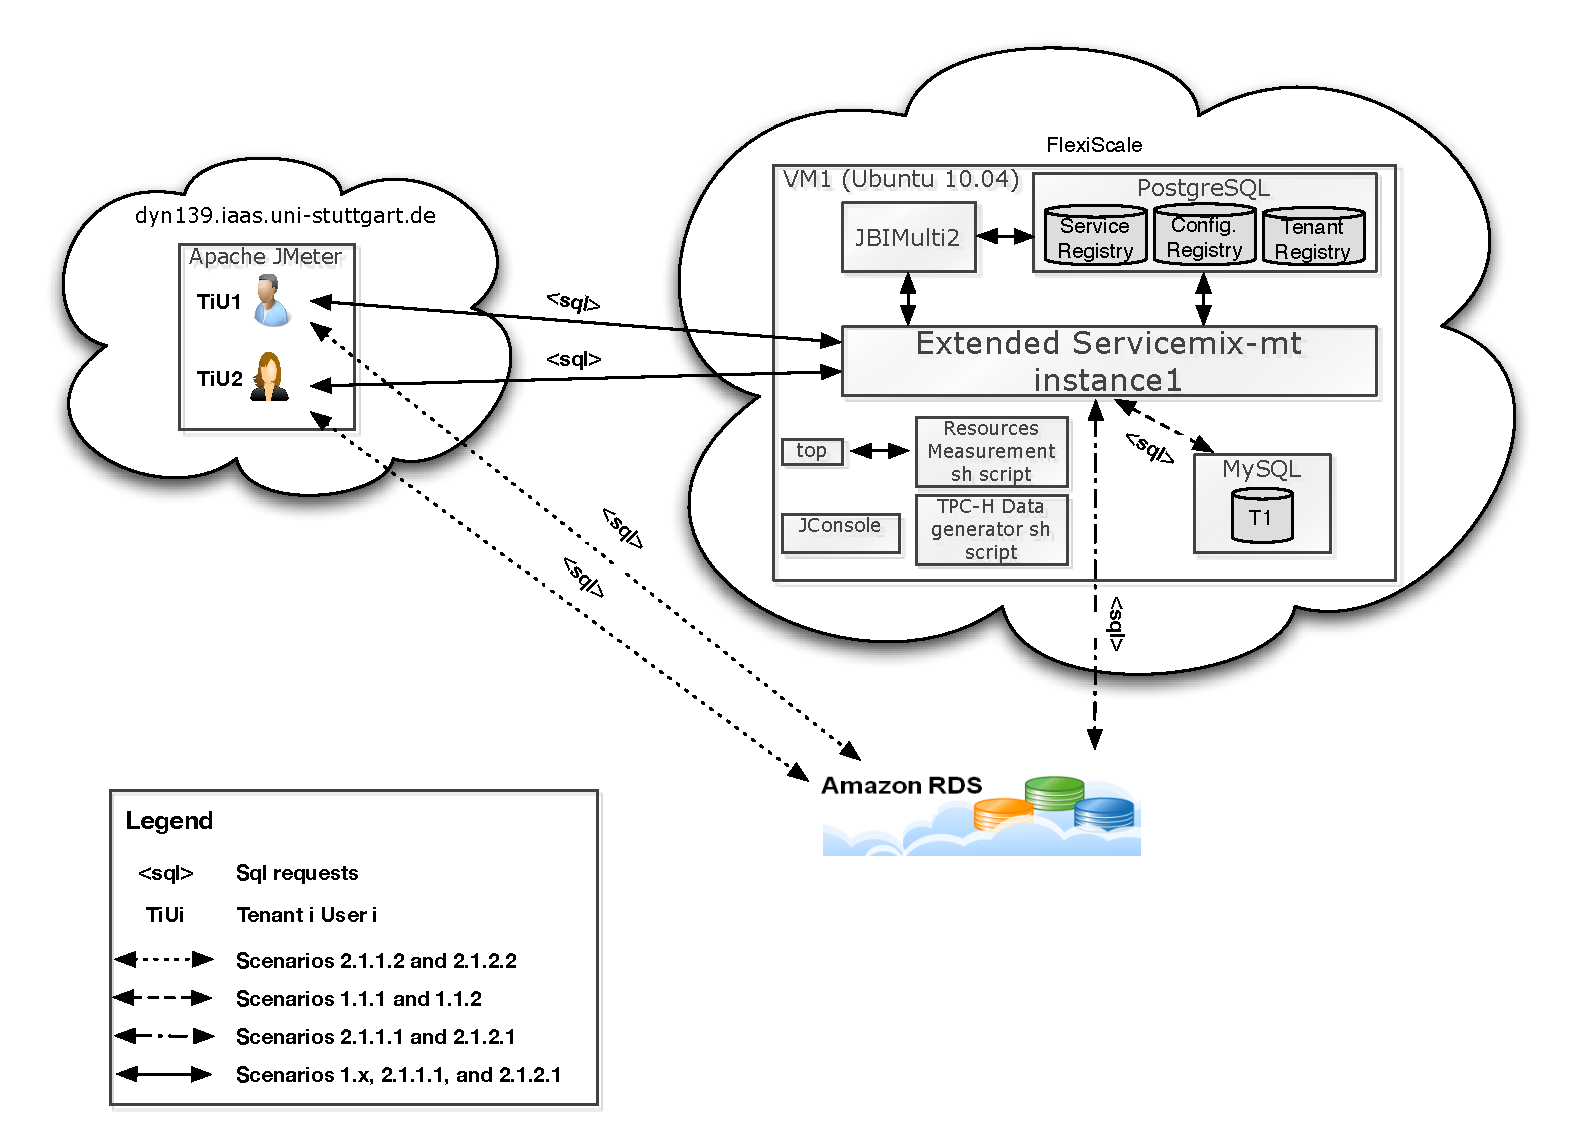
\includegraphics[width=0.7\textwidth, trim=0.0cm 0.0cm 0.0cm 0.0cm, clip]{./gfx/evaluationoverview.pdf}
	\caption[Performance Evaluation Components Overview]{Overview of the components used for the \ac{ESB} performance evaluation. \textbf{Note:} In the evaluation two different monitors are used. For communication the monitoring requires the counting and visualization of the incoming and outgoing requests. For system monitoring, the CPU and Memory usage should be measured.}
	\label{fig:evaluationoverview}
\end{figure}

\FloatBarrier

\FloatBarrier
\section{ESB Performance Evaluation Architecture}
\label{sec:esbevaluationdesign}

% explain the figure
% the evaluation is done for SOAP over HTTP protocols based on a in only message exchange patter, so that we are only masuring how much time does it take to reach the backend service. explain that the dashed lines are because those calls are optional, this means, we divide in to more than one scenario, each scenario testing 1, 2, 4, and 10 endpoints
% for the two instances of servicemix, we provide 10 endpoints in total, and 5in each instance, and the load is divided into the endpoitns. we start with the scenario with 2 endpoints
% explain a little bit the java bench androitlogic driver
% explain that we will use differente messages for the scenarios so that we can decouple them from the scenarios, being able to modify messages independently. results are in a format (I can paste an example of a result from the java benchmark) and then the driver provided by androit to be able to convert it to a csv file
% for concurrent calls between endpoints, we are going to create as many instances of the java benchmark as many endpoints we want to call concurrently by using shell scripting and the & (background task). Explain how many messages we are sending, in factor 2..., and the warmup phase of the esb, so that we ensure that the heap mamory is cleaned (garbage collector)
% system monitoring for the %CPU and %sys memory using the top command and then converting the output data to csv
% jconsole usage for heap measurements
% wireshark just for counting the packages that arrived and pack lost
% to fill the messages, we fill it with random characters and create a <attachment> part in the body

AndroitLogic has developed in their \ac{ESB} Performance Evaluation Round 3 a load generator for different scenarios. After analyzing its main features, we found it suitable for our work, but only if we can include tenant-awareness in the execution. We evaluate the \ac{SOAP} over \ac{HTTP} communication protocol in both native ServiceMix \ac{HTTP} \ac{BC} and in the multi-tenant \ac{HTTP} \ac{BC}. With this we want to evaluate not only the performance of the \ac{ESB} solution we are using in our Cloud infrastructure, but also the penalty caused by the multi-tenant awareness implementation. The \ac{SOAP} over \ac{HTTP} protocol is well known for its usage in Web services. In this evaluation we use as a backend Web service an Echo Service which logs the received requests. For this purpose, we must push the scenarios as close as possible to a real Web service consumption. Therefore, we divide the evaluation system in two virtual machines connected by a network (see Figure \ref{fig:evaluationarchitecture}). 


%%%%%%%%%%%%%%%%%%%%%%%%%%%%%
\begin{figure}[htb]
	\centering
		\includegraphics[width=.95\textwidth, trim=0.0cm 0.0cm 0.0cm 0.0cm, clip]{./gfx/evaluationarchitecture.pdf}
	\caption[ESB Performance Evaluation Architecture]{Architectural overview of the components used for the evaluation of the \ac{ESB} performance. \textbf{Note:} We evaluate only ServiceMix, not the integrated version of ServiceMix with the JBIMulti2 application, in order to be able to perform a direct comparison between the multi-tenant and the non multi-tenant ServiceMix.}
	\label{fig:evaluationarchitecture}
\end{figure}
%%%%%%%%%%%%%%%%%%%%%%%%%%%%%


The virtual machine one hosts the front and backends components: performance benchmark and the Web service. The Web service is deployed in an Apache Tomcat server. The extended performance benchmark is built of the following components: AndroitLogic driver, shell scripts and data converters. The AndroitLogic driver support concurrent users invoking the same endpoint, but not concurrent users between two or more endpoints. Furthermore, it does not support message modification for including tenant information. For this purpose, we have designed the shell scripts which can give support on those two requirements (see Figure \ref{fig:evaluationarchitecture}). In the first place, the shell script modifies or does not modify the message which will be sent by the driver. In the second place, we perform concurrent invocations between endpoints by creating several Unix background tasks of the driver. Each of the tasks results can be dumped in a shared file between the driver instances. However, the results come in non structured format for analysis. Therefore, we convert the data using a converter provided by AndroitLogic \cite{androit2012}. For monitoring the packet lost rate, we will listen on the server's port where the Web service listens with a well known monitoring tool, Wireshark \cite{wireshark}.

We use the virtual machines two and three for hosting the ServiceMix instances. The two instances are used only in non multi-tenant scenarios. For both multi-tenant and non multi-tenant scenarios we must increase the number of concurrent calls to the endpoints. In the requirement we specify scenarios of one, two, four, and ten endpoints. The system performance measurement can be done by system commands. We provide a component which take CPU and Memory measurements and converts its output to structured data for analysis. However, the system memory usage measurements do not give variable percentages over time. The percentage shown is the one associated with the memory consumption of the JVM the \ac{ESB} runs on, which is previously reserved and fixed over time. To get more representative data, we measure the heap consumption of ServiceMix in the JVM using Java Console, which give us a better representation of the variability between the different scenarios (See Figure \ref{fig:evaluationarchitecture}). For monitoring the communication, an instance of Wireshark can also be used, but in our evaluation it is optional.


\FloatBarrier
\clearpage
\section{Evaluation}
\label{sec:evaluation}

In this section we first describe the components we implemented to be able to reuse the existing load performance driver from AndroitLogic \ac{ESB} Performance Round 6 and adapt it to the required multi-tenant scenarios \cite{androit2012}. In Section \ref{sec:evaluationanalysis} we shortly describe the deployment and initialization in the virtual machines under the Flexiscale network \cite{flexiscale} and we evaluate the results obtained from the different scenarios. 

\subsection{ESB Performance Evaluation Benchmark}
% put a figure of the folder skeleton
% explain the androit benchmark (we can put an example of the inputs of the java call)
% explain the endpoint configuration (both multi-tenant and non multi-tenant)
% echo service at the end
% message sample (and explain that we will use the message sample to include the tenant id and user id in the to and from values) so that we can see them in the echo service
% endpoint configuration, for both multi tenant and non multi tenant

AndoitLogic has developed an ESB Performance Benchmark in their Round 6 \cite{androit2012}. Their benchmark evaluates the ServiceMix behavior under different scenarios, which vary in the request message size, number of requests per endpoint, and number of concurrent users per endpoint. Their load generator is included in the \term{org.adroitlogic.toolbox.javabench} package in their Management Toolbox application \cite{androit2012}. They provide an HttpBenchmark and a \term{data to csv format} converter. The former makes \ac{HTTP} POST requests to the specified endpoint URL, and generates performance statistics, e.g. response time, throughput. The latter converts the driver's results to structured data for analysis. We reuse both components, but develop components on top which create several instances of the \term{javabench} to invoke multiple endpoints concurrently. Furthermore, we need to add tenant context information before invoking the driver. The components are implemented in UNIX shell scripts.

%%%%%%%%%%%%%%%%%%%%%%%%%%%%%
\begin{figure}[htb]
	\centering
		\includegraphics[width=.95\textwidth, trim=0.0cm 0.0cm 0.0cm 0.0cm, clip]{./gfx/folderorganizationesbperformance.pdf}
	\caption[ESB Performance Evaluation Package Structure]{Overview of the package used for the evaluation of the \ac{ESB} performance}
	\label{fig:folderarch}
\end{figure}
%%%%%%%%%%%%%%%%%%%%%%%%%%%%%

In Figure \ref{fig:folderarch} we describe the overall structure of our loader package. We define three scenarios: scenario 1 is non multi-tenant aware and with one instance of ServiceMix, scenario 2 is non multi-tenant aware with two instances of ServiceMix, and scenario 3 is multi-tenant aware with 1 instance of ServiceMix \cite{EvalESB}, \cite{EnablingMT}. The \ac{SOAP} messages and the endpoints' URLs are read from \ac{XML} files stored in the \term{scenariox} folder. The messages vary from 500B to 100K. However, in this student thesis we perform the analysis for the 500B and 1K messages' sizes. The main and secondary scripts used in this analysis are located under the main scripts folders and the results generated are stored in the \term{ResultsScenariox} folder. In addition, for the multi-tenant scenarios, the endpoint URL file must also contain the tenant context information, e.g. tenantId and userId. 

For the evaluation scenarios we create using the ServiceMix \ac{HTTP} maven archetype 11 \ac{SU}s. Ten \ac{SU}s contain non multi-tenant endpoint configurations of 10 consumer and 10 providers which support the \ac{SOAP} over \ac{HTTP} communication protocol, while one \ac{SU} is configured to be deployed on the multi-tenant \ac{HTTP} \ac{BC} by 10 tenants, generating 10 tenant-aware endpoints (10 tenant-aware consumer and provider endpoints). The deployment phase is described in Section \ref{sec:evaluationanalysis}.

%%%%%%%%%%%%%%%%%%%%%%%%%%%%%
\lstinputlisting[label={lst:scenarioinvokationi},caption={[ESB Performance Analysis Main Shell Script Invocation] Invocation parameters in the main shell scripts of the benchmark.},basicstyle=\scriptsize]{./gfx/androitinvokation.txt}
%%%%%%%%%%%%%%%%%%%%%%%%%%%%%

For the non multi-tenant scenarios, we specify the needed invocation parameters in Listings \ref{lst:scenarioinvokationi}, \ref{lst:loopinvokation}, and \ref{lst:loopinvokation2}. The non multi-tenant aware shell script takes as one of the input parameters the file path where the \ac{SOAP} message is stored and creates the result scenario file name based on the message size and the running scenario. Furthermore, the endpoints' URLs are retrieved from the endpoint configuration file and the script reads as many URLs as tenants we specify. For supporting concurrent calls between endpoints, we create as many instances of the \term{javabench} as endpoints by running a secondary script, the loop script (see Figure \ref{fig:folderarch}), which is executed as a Linux background task. The scenario is divided in two phases: warm-up and performance test. In the warm-up phase an amount of requests are concurrently sent to the endpoints in order to warm-up the \ac{ESB} and get consistent results, while in the performance test phase we perform the measurements which can be analyzed. In the warmup phase the initial request number is set to 10240 requests. This value is then increased exponentially, and divided by the number of endpoints, as described in the following explanation. The loop script increments exponentially the number of requests and divides it by the number of endpoints in the \ac{ESB}, e.g. during the performance test phase if an initial request number is set to 20, then it sends to each endpoint \begin{math} 20 * 2^i, i = [1,2,3,5,6] \end{math} divided by the number of invoked endpoints in the scenario. The same sequence is applied for the multi-tenant scenario. 

%%%%%%%%%%%%%%%%%%%%%%%%%%%%%
\lstinputlisting[label={lst:loopinvokation},caption={[ESB Performance Analysis Non Multi-tenant Shell Script Invocation]Invocation parameters in the non multi-tenant shell script of the benchmark.},basicstyle=\scriptsize]{./gfx/loopinvokation.txt}
%%%%%%%%%%%%%%%%%%%%%%%%%%%%%

The approaches taken into account for the non multi-tenant scenarios are similar to the multi-tenant scenario, as it is shown in Listing \ref{lst:loopinvokation}. The main difference relies on the need of tenant context information injection before the \ac{SOAP} message is read and sent over \ac{HTTP} concurrently to the tenant-aware endpoints. The concurrent reading of messages leads us to the need of using temporal files to store the messages containing tenant context information. The temporal files are created in the same directory as the requests files, and we modify the content by reading the original request in the loop2 script shown in Listing \ref{lst:loopinvokation2} and using the Linux \term{sed} command to inject the tenant context information read from the endpoints' URL definition file. 

%%%%%%%%%%%%%%%%%%%%%%%%%%%%%
\lstinputlisting[label={lst:loopinvokation2},caption={[ESB Performance Analysis Multi-tenant Shell Script Invocation]Invocation parameters in the multi-tenant shell script of the benchmark.},basicstyle=\scriptsize]{./gfx/loopinvokation2.txt}
%%%%%%%%%%%%%%%%%%%%%%%%%%%%%

With the above approaches we fulfill the requirement of getting the response time and the throughput when invoking and external Web service through an \ac{ESB}. We have also implemented scripts for monitoring the system resources with the \term{top} Linux command and with the Java Console \cite{jconsole}. The former provides data at the system level, e.g. JVM memory consumption, while the latter provides data about the exact amount of JVM resources the ServiceMix process consumes.


\subsection{ESB Performance Evaluation Analysis}
\label{sec:evaluationanalysis}

	In this student thesis we extend and add extra functionality to ServiceMix. Therefore we need to measure its behavior and compare it with the baseline, which is the non multi-tenant version of Apache ServiceMix 4.3.0 \cite{ASM}. In the following sections we describe the systems we use for evaluating the performance of the \ac{ESB}, and we discuss some of the results we obtained. 

	\subsubsection{Deployment and Initialization}
	
	The different scenarios we run in this evaluation must approximate as much as possible to real scenarios. Thus we utilize three Ubuntu 10.04 virtual machines in this evaluation connected by the network in the Flexiscale infrastructure \cite{flexiscale}. One virtual machine hosts the evaluation package and an echo Web service which implements the In-Only \ac{MEP} and is deployed in Tomcat 7.0.23. Wireshark 1.2.7 is installed for monitoring incoming and outgoing requests to and from the echo Web service. In a second and third virtual machine we install one instance of ServiceMix 4.3.0 and the system resources measurement scripts. We have listed in Section \ref{sec:evaluationspecification} a set of multi-tenant and non multi-tenant scenarios. For the non multi-tenant scenarios we have deployed in the ServiceMix \term{deploy} directory a \ac{SA} containing the configuration of 10 consumer and 10 provider endpoints. For the multi-tenant scenarios we performed the operations described in Section \ref{sec:multitenanttest} and deploy through JBIMulti2 10 tenant-aware consumer and 10 tenant-aware provider endpoints. Both tenant-aware and non tenant-aware endpoints must be specified in the endpoint file the extended driver reads for sending the \ac{SOAP} requests.
	
	
	\subsubsection{Evaluation Analysis}
	
	%%%%%%%%%%%%%%%%%%%%%%%%%%%%%
	\begin{figure}[htb]
		\centering
			\includegraphics[clip, scale=0.5]{./gfx/response1K.pdf}
		\caption[ESB Performance Evaluation Response time for 1KB Messages]{Response time of the different scenarios for 1KB \ac{SOAP} over \ac{HTTP} requests \cite{EvalESB}.}
		\label{fig:responsetime}
	\end{figure}
	%%%%%%%%%%%%%%%%%%%%%%%%%%%%%
	
	The numerical values obtained from the communication driver are distributed per endpoint. Therefore, we make the average between the endpoints for each set of sent requests. The latency when increasing the number of endpoints in the system increases between 25\% and 45\% for concurrent requests sent to 2, 4 and 10 endpoints (see Figure \ref{fig:responsetime}). We can see that our extended version declines the original ServiceMix's performance approximately 30\% \cite{EvalESB}. Furthermore, we can observe that the response time for the different multi-tenant scenarios does not increase proportional to the number of tenants, but shows a better performance per endpoint. When distributing the requests between two ServiceMix instances we have observed that the response time is substantially reduced when increasing the number of endpoints.	
	
	%%%%%%%%%%%%%%%%%%%%%%%%%%%%%
	\begin{figure}[htb]
		\centering
			\includegraphics[clip, scale=0.7]{./gfx/evaluation_throughput.pdf}
		\caption[ESB Performance Evaluation Throughput for 1KB Messages]{Throughput of the different scenarios for 1KB \ac{SOAP} over \ac{HTTP} requests \cite{EvalESB}.}
		\label{fig:evaluationthroughput}
	\end{figure}
	%%%%%%%%%%%%%%%%%%%%%%%%%%%%%	
		
	When measuring the throughput, the analysis took us to the same deduction we discussed above. When the number of endpoints decreases, we can observe a bigger gap between the native and the extended version of ServiceMix. As we increase the number of endpoints, e.g. 10 endpoints, we can see that the gap between approaches is exponentially narrowed (see Figure \ref{fig:evaluationthroughput}).  
	
	%%%%%%%%%%%%%%%%%%%%%%%%%%%%%
	\begin{figure}[htb]
		\centering
			\includegraphics[clip, scale=0.5]{./gfx/evaluation_cpu.pdf}
		\caption[ESB Performance Evaluation CPU Consumption]{Overview of the CPU consumption over the different scenarios \cite{EvalESB}.}
		\label{fig:evaluationcpu}
	\end{figure}
	%%%%%%%%%%%%%%%%%%%%%%%%%%%%%
	
	Finally, we have analyzed the CPU consumption of the process running the ServiceMix instance. We can observe in the average CPU consumption that there is a gap between both multi-tenant and non multi-tenant scenarios which increases when the number of endpoints increases. However, when increasing the number of endpoints the average CPU consumption stabilizes and maintains close to a constant value. The maximum CPU consumption values decreases in the non multi-tenant scenarios when increasing the number of endpoints, while for the multi-tenant scenario it linearly increases from two endpoints. In the 4 or 10 endpoints scenarios, the maximum CPU consumption difference between the native and the extended approaches are between 250\% and 320\% approximately (see Figure \ref{fig:evaluationcpu}).

The tenant authentication procedure demands a greater number of resources when parsing the \ac{SOAP} headers and the \ac{XML} data from the tenant context file. However, this decline caused by the implemented authentication procedure and the marshaling of tenant context information within the process is much lower that the decline caused by establishing a connection with an external database system and retrieving the tenant context information from an external source to the process.  
	
	



\chapter{Outcome and Future Work}
\label{chap:outcome}
%What have we done??
% we have evaluated the different technologies that were used and the different components which were separately implemented. multi-protocol multi-tenant communication in servicemix (soap http, jms, email and camel), included authentication in the esb, confidentiality and integrity is still missing. integrated version with the taxi scenario and separate endpoints configuration for both testing scenarios that we run, one for the taxi scenario and one for testing the endpoints individually. two echo services for testing the implemented approaches and used afterwords for the esb performance analysis. an analysis of the performance of the esb solution we are using and we have compared the penalty in the performance because of our modifications. we have also compared the actual performance improvement of distributing the load between two instances of servicemix and realized that is not a 50 % improved, this leads to a higher cost and less proportional improvement.  

Migration of one or more application layers to the Cloud aims to reduce the cost in the required IT infrastructure to host and maintain such layer within an organization. Adaptations on both migrated and non migrated layers are a must when part of an application is migrated to a Cloud infrastructure. In this diploma thesis we start from the basis of a partial migration of the application, particularly the database layer. The database layer includes the operations which provide data storage and retrieval support. Furthermore, the software, hardware and maintenance required to host and maintain this layer require an economical budget substantially greater than the needed for the business, or presentation layers of an application. Migrating the application's data to the Cloud requires rewiring the database connections to the backend Cloud data store, and adaptating the upper layers to match the operations, and data representations supported. Providing transparent communication support for accessing and storing data on application's databases in the Cloud demands a multi-protocol, and multi-tenant component. In this diploma thesis we extend a multi-tenant aware \ac{ESB} in order to utilize it as the database layer of the application, and access multiple Cloud data stores providing \ac{SQL} and \ac{NoSQL} databases. 

In Chapter \ref{chap:fundamentals} we present the necessary background about the technologies we use, and the components we reuse in this diploma thesis, e.g. JBIMulti2 \cite{Muhler2012}, \ac{JBI} and \ac{OSGi} frameworks, etc. Furthermore, we categorize the databases systems which are supported in the prototype, and subcategorize them based on their storage model and communication protocols. 

After researching on the \ac{SQL} and \ac{NoSQL} database systems properties in Chapters \ref{chap:fundamentals} and \ref{chap:relatedworks}, we find that most of database communication protocols are not standardized, and differ along the different database vendors. Therefore, we are forced in Chapter \ref{chap:design} to develop components which adjust to specific communication protocols: \ac{HTTP}, and MySQL. The research described in Chapter \ref{chap:relatedworks} leads us to find a lack of standardization in the communication at the TCP level of the \ac{SQL} database vendors, but the existence of components which support other communication protocols for incoming requests, e.g. \ac{HTTP}, and utilize via \ac{JDBC} the different database vendors' native driver to forward them to the backend database system \cite{jboss2011}. However, approaches in this direction forces the developer to adjust their data access layer, whose adaptations we aim to minimize when utilizing our system. \ac{NoSQL} Cloud data store providers show a lack of standardized naming, and provide the database users with their drivers for I/O operations. In order to address the lack of a standardized naming and access in the \ac{NoSQL} providers, we categorize in the system's registry the user's databases meta-data into different categories and subcategories, and access the backend data stores via the \ac{HTTP} protocol supported in ServiceMix-http-mt \cite{gomez2012}. 

The functional and non-functional requirements the system must fulfill are described in Chapter \ref{chap:spec}. After analyzing the requirements, providing an overview of the system, and specifying the necessary use cases, we move to the design of the prototype in Chapter \ref{chap:design}. We divide the design into the design of common components, and database specific components for the following databases types: \ac{SQL}, and \ac{NoSQL} databases. Apache ServiceMix-mt is used as the main component in the system for enabling a multi-protocol and multi-tenant communication support between backend databases. We design two different \ac{NMF}s' content for requests for enabling a dynamic routing of requests between the backend database systems. We extend the JBIMulti2 registries schemas to support the storage of tenant's migrated database configuration data. Components which implement the different databases systems communication protocols, e.g. MySQL and \ac{HTTP}, and components enabling routing between the multi-tenant aware consumer and provider endpoints are presented in Chapter \ref{chap:design}. However, the \ac{SQL} database support is limited in the system to one specific database system: MySQL. Separate components can be implemented to provide support for more \ac{SQL} database vendors, e.g. PostgreSQL or Oracle. Furthermore, the \ac{NoSQL} databases support is limited to the backend databases which support the \ac{HTTP} communication protocol. 

The implementation, validation, and evaluation of the system which complies with the requirements and the design of Chapters \ref{chap:spec} and \ref{chap:design} respectively, is explained in Chapters \ref{chap:implementation} and \ref{chap:validationevaluation}. We first validate the system by creating backend databases which contain custom data, and data generated by the TPC-H benchmark \cite{tcpbenchmark}. After configuring the communication configuration in CDASMix through the JBIMulti2 Web service interface, the tenant can communicate with the backend Cloud data store. Communication configuration should be done in the future through a user friendly Web interface, by integrating the \term{Cloud Data Migration Tool} and JBIMulti2 Web interfaces. 

For evaluating the advantages and disadvantages of utilizing CDASMix as the communication component in a database layer, we create an evaluation baseline for a backend MySQL database, run the different evaluation scenarios, and discuss its results. Applications with a high number of I/O operations often suffer a high performance decrease \cite{cashing2012}. Therefore, we enhance our prototype with a temporal multi-tenant cashing mechanism. Results describing the behavior of the system with a high load of data requests is described in Chapter \ref{chap:validationevaluation}, and demonstrate the advantages of cashing when accessing databases in the Cloud through CDASMix. An evaluation of the system's communication performance between \ac{NoSQL} databases is recommended in future works.

Further future works involve a secure authentication mechanism in CDASMix, as well as horizontal scalability of the system, and query transformation. The former involves implementing in the CDASMix MySQL Proxy the authentication mechanisms supported in the MySQL database server, and including password verification in the authentication phase in the multi-tenant \ac{HTTP} \ac{BC}. Horizontal scalability can be obtained between multiple instances of ServiceMix-mt building the system. Future versions of CDASMix can provide separate but connected ServiceMix-mt instances for routing requests for \ac{SQL} and \ac{NoSQL} database systems, or implementing a load balancer between the multiple instances building the data access layer. The developed version of CDASMix does not provide query and data transformation between different database versions, or database vendors. However, the system's design and implementation is extensible. A transformation component can be inserted between the endpoints in ServiceMix-mt.



%future work
%web gui, for both jbimulti2 and cloud data migration tool.-
% connection of the cloud data migration tool with the jbimulti2-
% benchmarking of the nosql
% benchmarking of the sql for more providers, and trying different configurations of database location and products and providers
% authentication in the system with the password
% support for incoming postgresql
% multiple instances of an esb connected to each other, and separate for example, one esb for sql, and one esb for nosql
% transformation of queries, and data

%The utilization of an \ac{ESB} as the main piece of middleware for \ac{SOA} in a Cloud environment forces multi-tenancy awareness to be a must in its requirements. This student thesis integrates the two main approaches for enabling multi-tenancy in an open source \ac{ESB}: multi-tenant aware messaging and multi-tenant aware administration and management, as well as analyzes and compares the performance of the native and extended \ac{ESB} solution in different scenarios, and produces as its main outcome an integrated version of the taxi application \cite{4CaaSt}. 

%In Chapter \ref{chap:fundamentals} we first provide the needed background on the technologies, communication protocols, and the main components this student thesis work with: ServiceMix and JBIMulti2 \cite{ASM}, \cite{Muhler2012}. After acquiring the main knowledge of the solutions, we investigate in Chapter \ref{chap:relatedworks} different solutions which support multi-tenancy, and analyze approaches which have been already taken into account. Furthermore, we discuss the supported functionalities of the AndoitLogic load generator driver, and the possibility of its reuse in our performance analysis. The identification of requirements and the system overview presented in Chapter \ref{chap:spec} guide us to perform the design of the different components of this student thesis in Chapter \ref{chap:design}. The design leads to a multi-tenant and multi-protocol aware version of ServiceMix, supporting three communication protocols: \ac{SOAP} over \ac{HTTP}, \ac{JMS}, and E-mail. Furthermore, we provide an integration design for the taxi application v2.0 prototype and we reengineer most of the implemented communication approaches in order to improve the system's performance and to add new functionalities, e.g. tenant context data structure modification, tenant authentication, and tenant-aware isolated endpoints in the \ac{ESB}. One of the main requirements in a Cloud infrastructure is security. We implement tenant authentication but not tenant data integrity and confidentiality. The tenant context information sent to and from the \ac{ESB} must be encrypted in future versions of the \ac{ESB}.

%Chapter \ref{chap:implementation} describes the challenges and approaches we faced for both the integration with the taxi scenario and the extension of the different \ac{JBI} \ac{BC}s. As discussed in Chapter \ref{chap:implementation}, one of the main goals we have in the improved version of the taxi application is to maximize the \ac{ESB} usage between components and to integrate a multi-tenant aware \ac{ESB} with non multi-tenant aware components which build part of the taxi application, e.g. \ac{BPEL} processes under Orchestra, CMF and GoogleDirections components, etc. This contrast forced us to perform changes in some of the taxi application components in order to adapt multi-tenancy at the communication level. Future versions of the taxi application should support multi-tenancy awareness in its components, and we consider that a bidirectional connection between JBIMulti2 and the taxi companies Web interfaces should be set in order to retrieve the tenant context information. Furthermore, the only communication protocol which actually supports the taxi application is the \ac{SOAP} over \ac{HTTP}. We have extended both \ac{JMS} and Mail \ac{JBI} \ac{BC}s for supporting a multi-protocol communication between customers and taxi drivers in a future version of the taxi application. This aspect directed us to build two different testing environments, one for the taxi application and one for the individual testing of the extended \ac{BC}s described in Chapter \ref{chap:test}.

%For analytical purposes after implementation, we perform an evaluation of the performance in Chapter \ref{chap:performanceevaluation} of both native and extended versions of ServiceMix. This student thesis reuses and extends an existing \ac{SOAP} over \ac{HTTP} \ac{ESB} performance benchmark. We adapt the benchmark to support multi-tenancy and evaluate the obtained results from different scenarios. However, we could not perform this analysis on more that one communication protocol. In the future it would be interesting to run the same scenarios on the \ac{XML} over \ac{JMS} communication protocol. Those results can give the \ac{ESB} administrator a better output for offering the communication protocols which best execute in our ServiceMix version. Furthermore, we perform the evaluation of one important scenario in a Cloud infrastructure: dividing the load between more than one ServiceMix instance by emulating a load balancer. The results showed that the performance is not significantly increased with the increase of the number of endpoints, and this approach can be not worth its expenditure. However, as we discussed, we emulate load balancing. For more than one instance of \ac{ESB} a load balancer should be integrated to the extended system. 

%Finally, we have integrated a multi-tenant \ac{ESB} which connect different endpoints via different protocols, e.g. external consumers with external providers. However, data is nowadays the most important asset of any business \cite{CHONGA2006}. The offering of a data-as-a-service solution in a Cloud environment where data can accessed through \ac{SOA} mechanisms, ables the use of the \ac{ESB} as a data access layer. With this approach data can be accessed from everywhere just by communicating with the \ac{ESB} and without worrying about the underlying architecture, e.g. database vendor, connection drivers. 



% Things to put: security in communication, JMS performance testing, using the ESB as Data Access Layer, optimization in the system resources usage of the actual implementation, load balancing between two or more instances of the esb, integration of the taxi scenario to communicate with jms or email, jms management of dominik improve it to have a bidirectional pipeline between jbimulti2 and servicemix, as well as connecting jbi multi2 with the taxi application and transmitter with security mechanisms in order to make a direct deployment of bcs from there or to just send the tenant and user information


\begin{appendix}


\chapter{Components}

%This chapter lists \ac{XSD}s that WS-Policy Assertion language and Rules XML file must conform. Furthermore, there are given several policy documents of Cloud data stores that are used for validation.

\section{CDASMix MySQL Proxy}
\label{appendix:cdasmixmysqlproxy}

The MySQL proxy \ac{OSGi} bundle is implemented on the Continuent Tungsten Connector \cite{tungstenwiki}, which is a Java MySQL proxy which directly connects with the backend MySQL database system. We extend and adapt this proxy in order to integrate it with ServiceMix, aggregate transparency, multi-tenant awareness, cashing, and dynamic connection with the backend Cloud data sources.

\begin{figure}[htb]
	\centering
		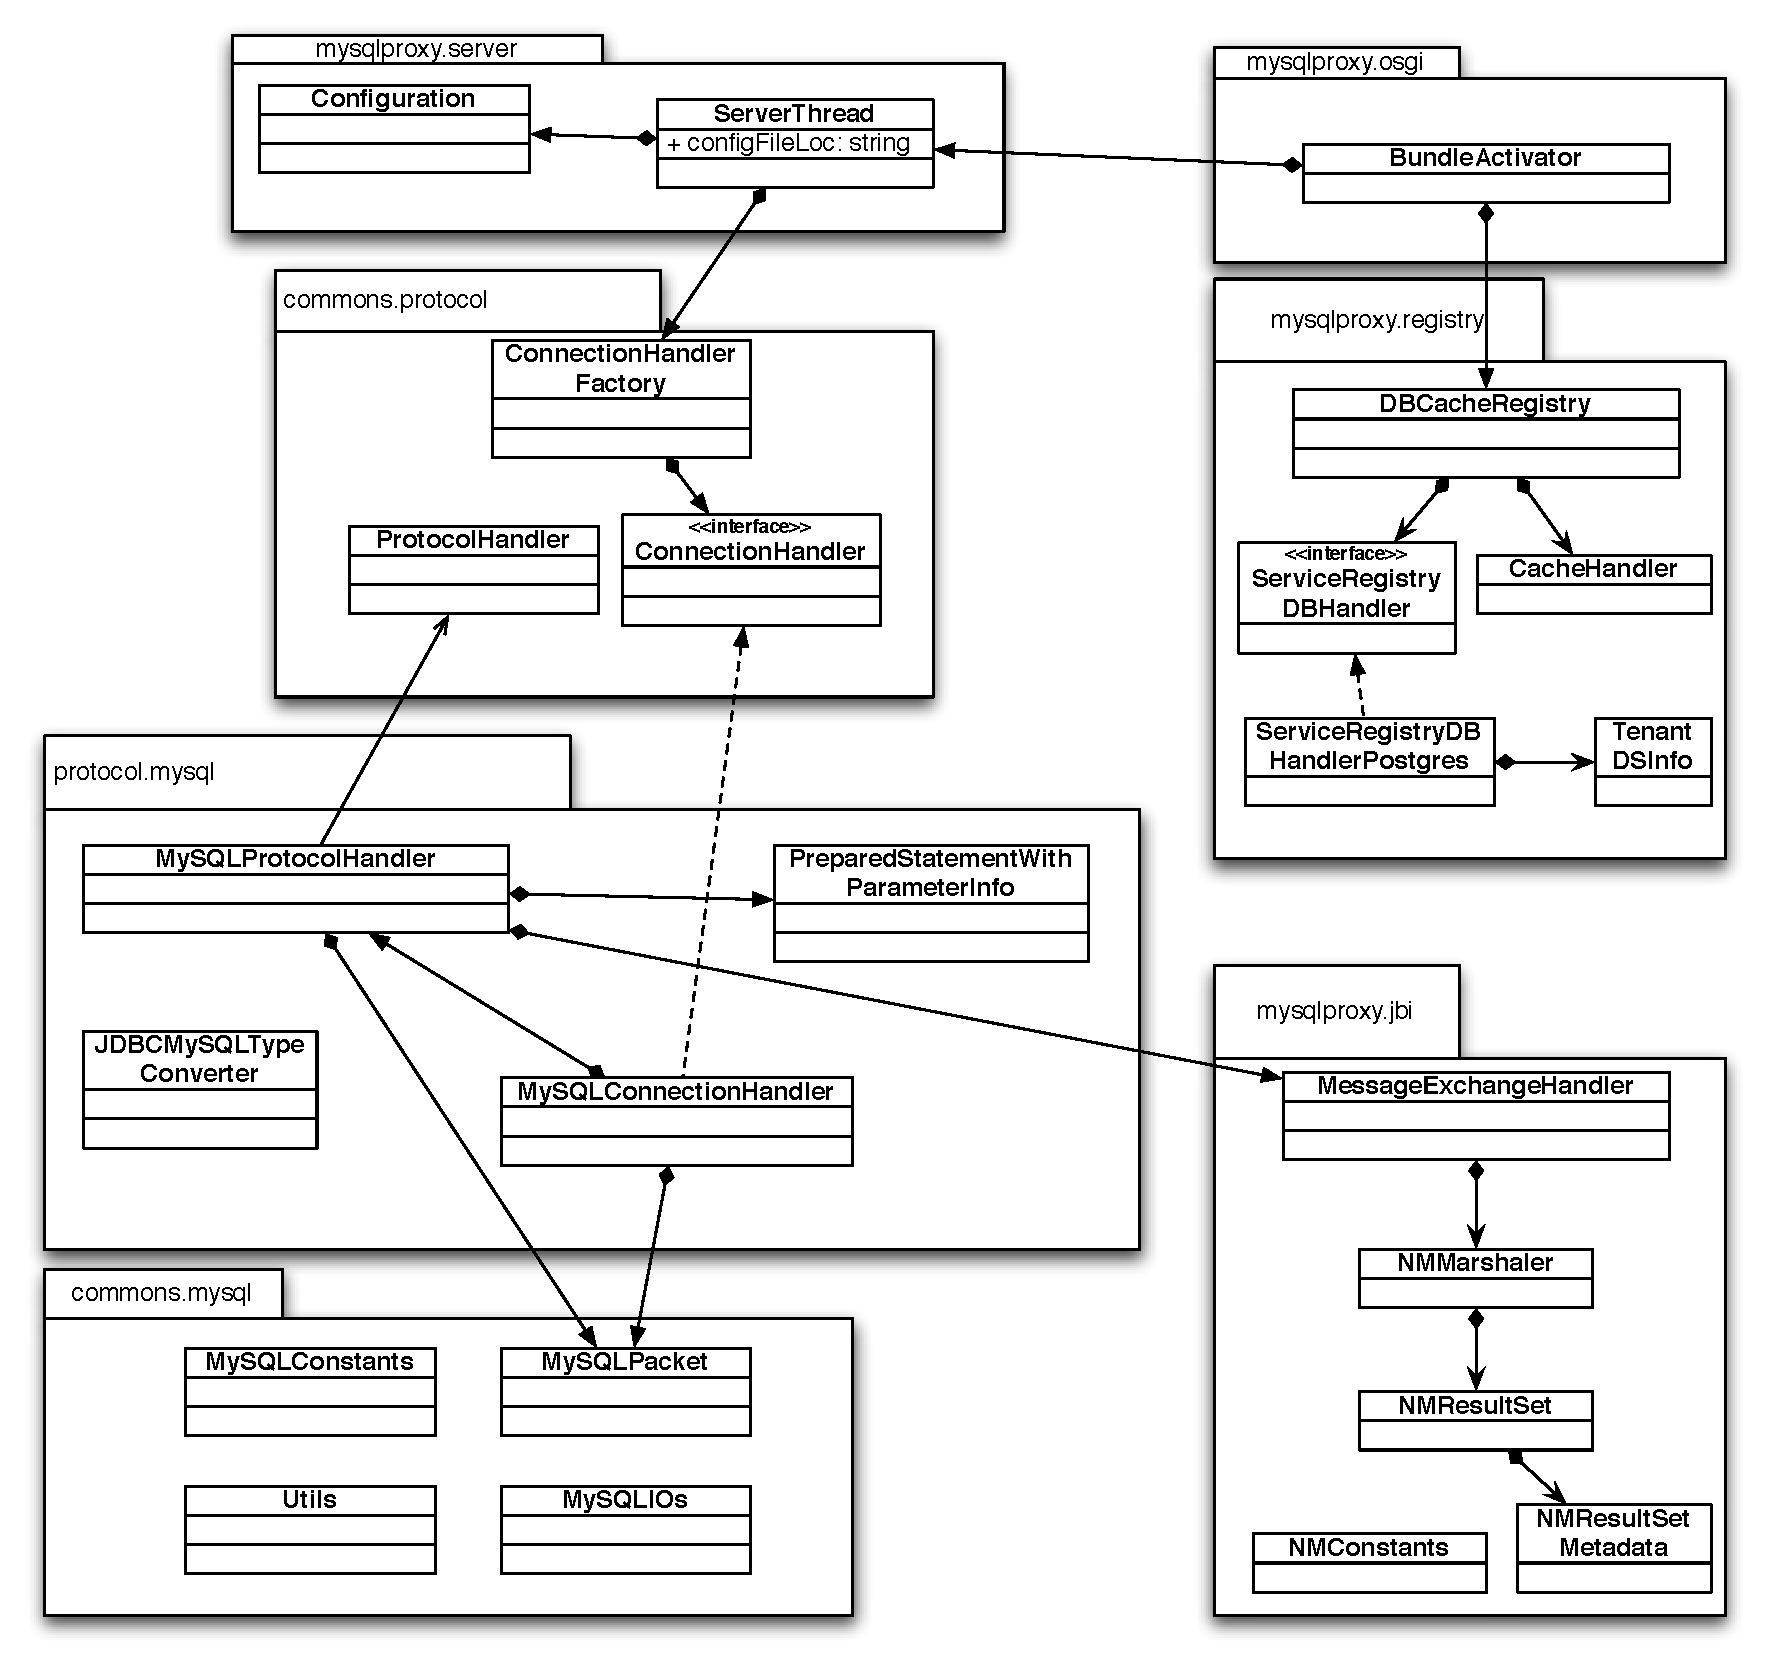
\includegraphics[clip, scale=0.4]{./gfx/mysql-osgi/mysql-proxy-v3.pdf}
	\caption[ServiceMix-mt MySQL OSGi Bundle]{OSGi bundle providing MySQL support in ServiceMix-mt}
	\label{fig:mysqlclassdiagram}
\end{figure}

\FloatBarrier

\vspace*{0.5cm}

%\lstinputlisting[label={lst:policy_language_syntax},caption={[Syntax of WS-Policy Assertion Language Schema]Syntax of WS-Policy Assertion Language Schema.},style=xml]{./gfx/master_thesis/cdhs-ws.xml}

%\vspace*{1cm}

%\vspace*{0.5cm}

%\lstinputlisting[label={lst:policy_language_schema},caption={[CDHS WS-Policy Assertion Language Schema]CDHS WS-Policy Assertion Language Schema.},style=xml]{./gfx/master_thesis/cdhs_properties.xsd}

%\vspace*{1cm}

\section{CDASMix Camel JDBC}
\label{subsec:cdasmixcameljdbc}

The \term{cdasmixjdbc} component is a custom component which is built and deployed as an \ac{OSGi} bundle in ServiceMix-mt. It provides support for connections with backend \ac{SQL} Cloud data stores, and message marshaling and demarshaling.

\begin{sidewaysfigure}[htb]
	\centering
		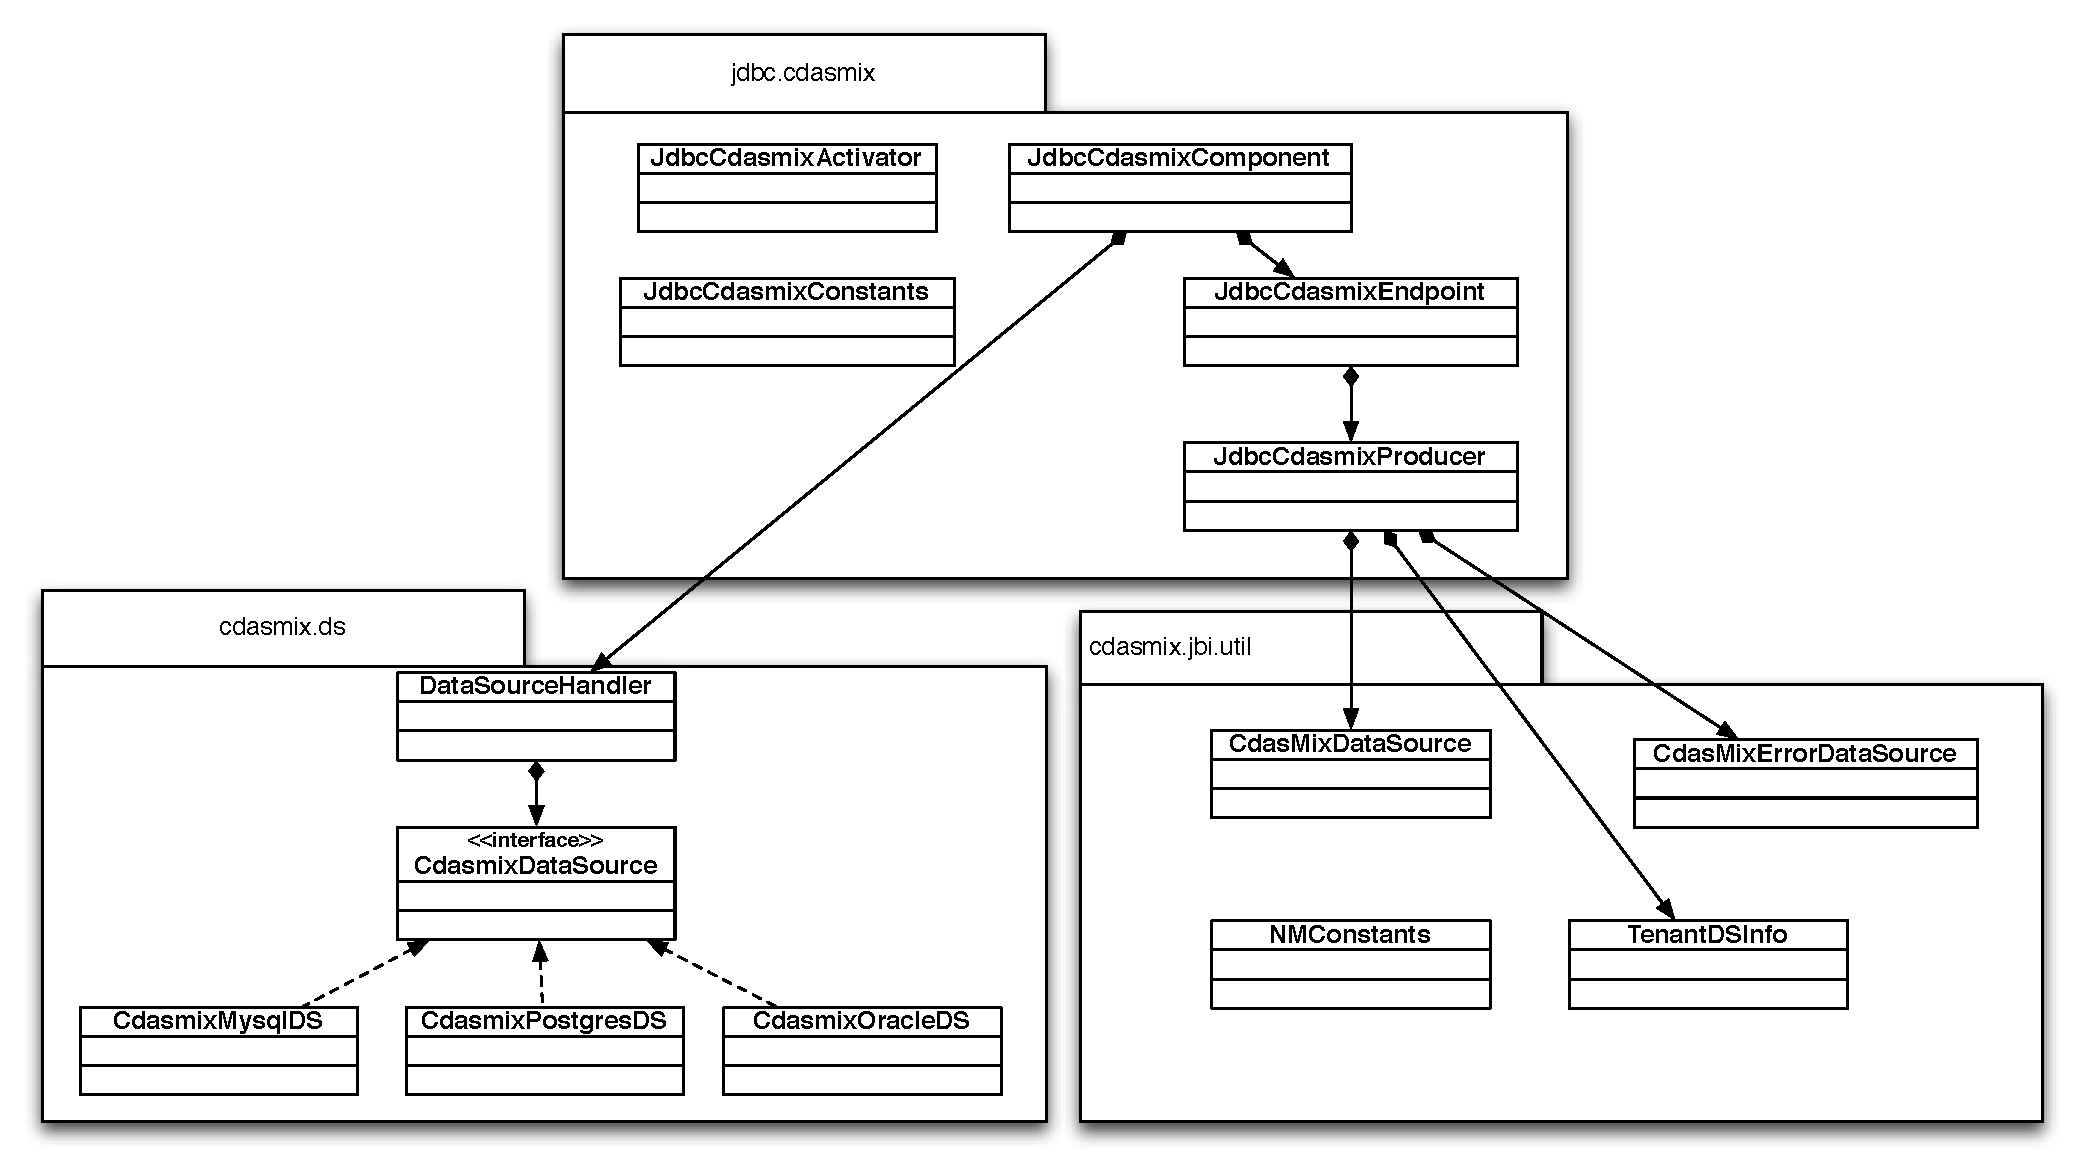
\includegraphics[clip, scale=0.6]{./gfx/cdasmix-camel-jdbc/cdasmix-camel-jdbc.pdf}
	\caption[ServiceMix-mt Camel CDASMix-JDBC Component]{OSGi bundle and Camel component providing JDBC support in ServiceMix-mt}
	\label{fig:cdasmixjdbcclassdiagram}
\end{sidewaysfigure}

\vspace*{0.5cm}

\FloatBarrier

%\lstinputlisting[label={lst:rules_schema},caption={[Post-Processing Rules XML Schema]Post-Processing Rules XML Schema.},style=xml]{./gfx/master_thesis/rules.xsd}

%\vspace*{1cm}

%\section{Multi-tenant ServiceMix HTTP Binding Component}
%\label{appendix:httpmtbc}

%to be filled
%\vspace*{0.5cm}

%\lstinputlisting[label={lst:googleCloudSQL-policy},caption={[Google Cloud SQL Service Provider Policy]Google Cloud SQL Service Provider Policy.},style=xml]{./gfx/master_thesis/provider_policies/GoogleCloudSQL.wspolicy}

%\vspace*{1cm}

%\vspace*{0.5cm}

%\lstinputlisting[label={lst:sqlDatabase-policy},caption={[SQL Database Service Provider Policy]SQL Database Service Provider Policy.},style=xml]{./gfx/master_thesis/provider_policies/SQLDatabase.wspolicy}

%\vspace*{1cm}
\FloatBarrier


\clearpage
\chapter{Messages}

%This chapter lists \ac{XSD}s that WS-Policy Assertion language and Rules XML file must conform. Furthermore, there are given several policy documents of Cloud data stores that are used for validation.
In this chapter we provide an overview of the requests which are sent to, and received from the extended ServiceMix-mt. For MySQL requests we provide the \ac{TCP} packets which are transferred between the application, ServiceMix-mt, and the backend MySQL database system. For NoSQL requests we present messages samples which are in \ac{JSON} format, but its content varies among the different backend Cloud data store providers. 

\section{Normalized Message Format Content Description}
\label{appendix:nmfcontent}

In this section we provide an overview of the data structures which are sent in the \ac{NMF}. The sections of the \ac{NMF} where the data and meta-data are sent are the \term{properties}, and the \term{attachment}.  In the Listing \ref{lst:nmfcontent} we detail the contents sent in each of the sections, and the data structures in which the data and meta-data are stored.

%\vspace*{0.5cm}

%\lstinputlisting[label={lst:policy_language_syntax},caption={[Syntax of WS-Policy Assertion Language Schema]Syntax of WS-Policy Assertion Language Schema.},style=xml]{./gfx/master_thesis/cdhs-ws.xml}

%\vspace*{1cm}
\vspace*{0.5cm}
%%%%%%%%%%%%%%%%%%%%%%%%%%%%%
\lstinputlisting[label={lst:nmfcontent},caption={[Data and Meta-data Detail in the Normalized Message Format]Detail of the content and data structures used to send the requests' data and meta-data.},style=ebnf]{./gfx/NMF_v3_0.txt}
%%%%%%%%%%%%%%%%%%%%%%%%%%%%%
\vspace*{1cm}

\section{MySQL TCP Stream}
\label{appendix:messagemysql}

In this section we provide two \ac{TCP} streams which are captured with the \term{ngrep} program for UNIX \cite{ngrep}. The first stream captures the \ac{TCP} packets on port 3311, where the MySQL component in ServiceMix-mt listens for incoming connections (see Listing \ref{lst:tcpstream3311}). The second stream captures the \ac{TCP} packets on port 3306, where the a locally deployed MySQL server listens for incoming connections (see Listing \ref{lst:tcpstream3306}).

%%%%%%%%%%%%%%%%%%%%%%%%%%%%%
\lstinputlisting[float=htb,label={lst:tcpstream3311},caption={[TCP Stream for a MySQL Communication Captured on Port 3311]TCP Stream for a MySQL communication captured on port 3311 with the program \term{ngrep} \cite{ngrep}.},style=ebnf]{./gfx/tcpstreamoutput3311.txt}
%%%%%%%%%%%%%%%%%%%%%%%%%%%%%

%%%%%%%%%%%%%%%%%%%%%%%%%%%%%
\lstinputlisting[float=htb,label={lst:tcpstream3306},caption={[TCP Stream for a MySQL Communication Captured on Port 3306]TCP Stream for a MySQL communication captured on port 3306 with the program \term{ngrep} \cite{ngrep}.},style=ebnf]{./gfx/tcpstream3306.txt}
%%%%%%%%%%%%%%%%%%%%%%%%%%%%%

\vspace*{0.5cm}

%\lstinputlisting[label={lst:policy_language_syntax},caption={[Syntax of WS-Policy Assertion Language Schema]Syntax of WS-Policy Assertion Language Schema.},style=xml]{./gfx/master_thesis/cdhs-ws.xml}

\vspace*{1cm}

\vspace*{0.5cm}

%\lstinputlisting[label={lst:policy_language_schema},caption={[CDHS WS-Policy Assertion Language Schema]CDHS WS-Policy Assertion Language Schema.},style=xml]{./gfx/master_thesis/cdhs_properties.xsd}

\vspace*{1cm}

\FloatBarrier


%\section{JSON in POST Request}
%\label{subsec:jsonpost}

%to be filled

\vspace*{0.5cm}

%\lstinputlisting[label={lst:rules_schema},caption={[Post-Processing Rules XML Schema]Post-Processing Rules XML Schema.},style=xml]{./gfx/master_thesis/rules.xsd}

\vspace*{1cm}

\FloatBarrier

\clearpage

\end{appendix}

\bibliographystyle{alphancex}
\bibliography{literatur/literatur}

All links were last followed on March 21, 2013.

\clearpage
\pagestyle{empty}
\vspace{9cm}
\begin{center}
\begin{minipage}{11cm}
\vspace{6cm}

\textbf{\Large Acknowledgement}\\\\
I am heartily thankful to my supervisor Steve Strauch from the University of Stuttgart for his encouragement, guidance and support in all the phases of this diploma thesis. I am also grateful to Dr. Vasilios Andrikopoulos for his advices and useful tips.
Special thanks to my family, friends and girlfriend for their moral support.

\vspace{1cm}
Santiago G\'omez S\'aez

\end{minipage}
\end{center}

\clearpage
\pagestyle{empty}
\vspace{9cm}
\begin{center}
\begin{minipage}{11cm}
\vspace{6cm}

\textbf{\Large Declaration}\\\\
\vspace{0.4cm}

All the work contained within this thesis,
except where otherwise acknowledged, was
solely the effort of the author. At no
stage was any collaboration entered into
with any other party.
\vspace{1cm}

Stuttgart, 22nd March 2013 \hspace{1cm}--------------------------------\\
\phantom{Stuttgart, March 22 2013} \hspace{1.3cm} (Santiago G\'omez S\'aez)
\end{minipage}
\end{center}

\end{document}
